\documentclass[10pt,twoside]{report}

%\usepackage[a4paper, hmargin={3.0cm, 3.0cm}, vmargin={2.5cm, 2.5cm}]{geometry}
\usepackage[a4paper,width=130mm,top=33mm,bottom=33mm,bindingoffset=6mm]{geometry}
% \usepackage{lmodern}
% \usepackage[T1]{fontenc}
%\usepackage{hfoldsty} % Computer Modern with osf
%http://www.khirevich.com/latex/font/
%http://www.tug.dk/FontCatalogue/

%before width=150 and top bottom = 25
% Use utf-8 encoding for foreign characters
\usepackage[utf8]{inputenc}

% packages
\usepackage{float}
\usepackage{color}
\usepackage{xcolor}
\usepackage{amsmath}
\usepackage{listings}% Package for including code in the document
\usepackage[pdftex]{graphicx}
\usepackage{caption}  % include figures and subfigures
\usepackage{subcaption}% include figures and subfigures
\usepackage{eso-pic} % \AddToShipoutPicture
\usepackage{fancyhdr}
\usepackage{pdfpages}
\usepackage{hyperref}		%include urls
\usepackage{url}			%include urls




%set listings to annotate Objective -C codeb
\lstset{language=[Objective]C,
		breaklines=true,
		xleftmargin=\parindent,
		showstringspaces=false,
		basicstyle=\footnotesize\ttfamily,
		keywordstyle=\bfseries\color{green!40!black},
		identifierstyle=\color{blue},
 }	


% Format Header and Footer
\pagestyle{fancy}
\fancyhead{}	% clear all header fields
\fancyhead[RO,LE]{Fat Finger - Simmulated Pressure}
\fancyfoot{}	% clear all footer fields
\fancyfoot[LE,RO]{\thepage}
\fancyfoot[LO,CE]{Chapter \thechapter}
\fancyfoot[CO,RE]{Tzemis Evangelos}
\renewcommand{\headrulewidth}{0.4pt}	% width of the line on header
\renewcommand{\footrulewidth}{0.4pt}	% width of the line on footer

%%% Override plain style
\fancypagestyle{plain}{%
  \fancyhf{}%
  \fancyfoot[LE,RO]{\thepage}%
  \renewcommand{\headrulewidth}{0pt}% Line at the header invisible
  \renewcommand{\footrulewidth}{0pt}% Line at the footer visible
}


% Title Formating of Thesis
\title{\textbf{University of Copenhagen} \\ 
 	\textbf{Master thesis dissertation} \\
 	 \textbf{Fat Finger}}

\author{ \textbf{Name:} \\ Evangelos Tzemis : khb107@alumni.ku.dk 
\\ \textbf{Supervisor:} \\ Sebastian Boring}


\setlength{\parindent}{0pt}
\setlength{\parskip}{2ex}
\linespread{1.2}


%%
%%
%% Cover Image
%%
%%
\begin{document}

\AddToShipoutPicture*{\put(0,0){\includegraphics*[viewport=0 0 700 600]{frontback/nat-farve}}}
\AddToShipoutPicture*{\put(0,602){\includegraphics*[viewport=0 600 700 1600]{frontback/nat-farve}}}
%\AddToShipoutPicture*{\put(0,0){\includegraphics*{frontback/nat-en}}}
\thispagestyle{empty}
\maketitle

%%
%%	Format all the preface
%%
\pagestyle{plain}
\cleardoublepage

\chapter*{Abstract}

Modern mobile and tablet devices, are operated through a set of multi-finger interactions, which are supposed to make interaction less confused, more natural and as seamless ad possible.
Despite the vast increase and evolution of the ways we interact with our mobile devices over the past yeas, the basic principle has remained the same, resulting in using only the on screen position of the fingers touching the screen.
We propose Fat Finger, that will additionally make use of the contact size of the finger touching the screen.
We developed an application in the form of target selection tasks and performed a user study where users had to succwssfully go through a series of different target selection trials.





\cleardoublepage


\chapter*{Dedication}
To my golden fish..
\cleardoublepage


% \chapter*{Declaration}
% I declare that..
\chapter*{Acknowledgements}
I want to thank...
\cleardoublepage

\tableofcontents
\cleardoublepage

\listoffigures
\cleardoublepage

\listoftables
\cleardoublepage

%%
%%	Chapter Formating
%%

\pagestyle{fancy}

\chapter{Introduction}
\label{sec:Introduction}
%%%%%%%%%%%%%%%%%%%%%%%%%%%%%
%%%%%%%%%%%%%%%%%%%%%%%%%%%%%
%%%%%%%%%%%%%%%%%%%%%%%%%%%%%
%%%%%%%%%%%%%%%%%%%%%%%%%%%%%
%%%%%%%%%%%%%%%%%%%%%%%%%%%%%
%%%%%%%%%%%%%%%%%%%%%%%%%%%%%
\section{Introduction}
Over the last few years, mobile and tablet devices, have become an indispensable part of our every day life. 
We mainly use them to communicate with others (Skype, FaceTime, chatting), surf the World Wide Web \cite{www}, read documents, and play video games. 
Tablet devices have also been assimilated in various working environments, providing a simpler, more accurate and direct way to monitor results, present graphs, and manipulate data by utilizing the touch motion and the device's portability.
Due to this variety of usage, most manufactures (Apple, Samsung, Google, LG etc.), continuously update their models with improved hardware and software to perfect match the user needs.
Since tablets devices and smartphones do not include any physical keyboard, numerous new techniques have been introduced to overcome this issue. The idea behind those approaches is: \emph{"Give Meaning to Touch"}. Introduction of gestures and multi-finger interaction \cite{multiTouch} has partly solved this problem. However, as we realize, we are always seeking for a more compact and robust approach, which will provide us the necessary tools for seamless and fluent interaction with our mobile devices. This lead us the following (rhetorical) question:

\emph{"Is the way we interact with mobile devices the most effective one? If not, how can it be improved?"}

Modern mobile devices are touch-based, allowing users to navigate through the interface using their finger, and type-in using a virtual keyboard. 
In the beginning, back to when the first commercial tablets were born, interaction was based on single-finger input. User interface was based on buttons and users had to select the corresponding buttons to perform discrete actions.
Recently, Multi-Finger interaction has been introduced, trying to emulate and simulate the behaviour of objects. This intends to make the user-interface more natural and improve users experience. 
Styluses have also been used to provide input on tablet devices. They are meant to assist users in performing more complex and accurate tasks (as drawing - designing), while some of them are even equipped with pressure sensitive sensors that detect the pressure applied and can be utilized by drawing applications (e.g. Photoshop) to control stroke width, or similar. 
Application-wise there are several applications in the App Store, Google Play etc. that use all those different kind of gestures to make complex tasks seem less confused. However users have to keep track of all those different gestures, and in case the application is not carefully designed, gestures will become cumbersome. For example, one finger for panning, blending into a two-finger pinch gesture for zooming, or even a three-finger drag to change modes in specific applications.  
From now on we will refer to interaction techniques that use only the position (x-y coordinates) of the finger(s) for providing basic input to tablet devices as \textbf{2D interaction techniques}, and to those that might use 2D interaction plus something extra (pressure, simulated pressure, vibration absorption) as \textbf{3D interaction techniques}.
Taking everything into consideration, I strongly believe that tablet devices are capable of providing even more natural ways for manipulating the content on them, and this is what I am seeking for in this thesis dissertation. I am proposing the Fat Finger interaction technique which exploits the contact size of the finger touching the screen, and thus belongs to the 3D interaction techniques. It adds a degree of freedom, which could later be used to integrate multi-finger drag gestures into a single fluid interaction, or just enhance the current ways we interact with tablet or mobile devices. 


%%%%%%%%%%%%%%%%%%%%%%%%%%%%%
%%%%%%%%%%%%%%%%%%%%%%%%%%%%%
%%%%%%%%%%%%%%%%%%%%%%%%%%%%%
%%%%%%%%%%%%%%%%%%%%%%%%%%%%%
%%%%%%%%%%%%%%%%%%%%%%%%%%%%%
%%%%%%%%%%%%%%%%%%%%%%%%%%%%%
\section{2D Interaction Techniques Evolution}


During the past years, the ways we use and provide input to our mobile devices have been vastly changed and evolved. The first input interface we meet is the simple 10 button keypad. Each button represents a number and a set of characters. Help buttons (as "*", "\#", "accept call" and "end call" ) were also provided. Whilst typing in such devices was cumbersome, continuous training and exposure to the interface made certain users develop high level technique, resulting in super-fast typing. 
In other more recent mobile devices we meet a mobile keyboard with much more buttons, called QWERTY \cite{qwerty}. Now, users had one-to-one correspondence between buttons and letters. However, due to the phone's size limitations, buttons were too small, making typing inefficient at certain circumstances.
To increase usability in old-style phones, a new typing technique was developed. Using a dictionary-based typing system, the necessary buttons clicks needed to type any kind of text, were vastly decreased. Thus, typing speed improved, even with a very simple number-based keypad. 

With the release of the first iPhone \cite{iphone} in 2007, the industry of smartphones, gained massive adoption. Smartphones can be thought as augmented featured normal phones. The iPhone was one of the first mobile phones to use a multi-touch interface, and the finger as the main source of input. Modern smartphones does not include a physical keyboard. 
So now, instead of providing input through the keypad, virtual keyboards and touch events were introduced. 

%tablet
Tablets followed the release of smartphones. A tablet is a portable computer with a touch sensitive display. It is usually equipped with cameras (front \& back), microphones, accelerometer, gyroscope, Touch ID \cite{touchID} etc. It provides touch input capabilities that can either be utilized using finger or a stylus. For text-entry, apart from handwriting recognition they also offer virtual on-screen keyboards. Finally their screen size is typically between 7'' and 10.1''.
The first tablet device was commercially available in 1989 from GRiD systems and was named GRiDPad. Until 2010, many companies have released their own version of tablet, most of them using resistive stylus driven screens. Resistive screens allow a high level of precision and are definitely preferred when used with a stylus.
After 2010 tablets use capacitive touch-screens, which allows for multi-finger interaction, and avoid the use of styluses. This allows integrated hand \& eye operation, since there is neither a stylus or a mouse to interfere. They also use ARM processors from improved battery life. Apple iPad was the product that defined the class of tablets and shaped the commercial market when launched, back in 2010. It runs iOS, a mobile version of MacOS, specifically designed for finger use, avoiding stylus requirements. 

Above we observed that many things changed through the past years in the commercial products, both addressing the mobile phones and the tablet devices. However  the principle we use to interact with all those mobile or tablet devices, did not really evolved.
 The interaction in only 2 Dimensional. In older keypads, the dimensions are the buttons and a boolean value which represents if a specific button is being touched or not.  
When operating on touch screens, we only get the x-y (2D) coordinates representing the point(s) we are touching on the screen.
Using multi-touch, we can now combine multiple fingers to perform more complex operations, which proved to be very effective. This is mainly because most of the gestures, movements and gestures we would do with physical objects, just transferred to the virtual environment. The most commonly used gestures are: Tap, Double Tap, Long Press, Scroll, Pan, Flick Two Finger Tap, Two Finger Scroll,  Pinch, Zoom and Rotate.
Despite the flexibility multi-finger provide us, 2D principle still holds because we only utilize the position of each finger touching the screen, and not other parameters as contact size, orientation, tilt, etc. Taking everything into consideration, I believe that we need to exploit the capabilities of all those modern devices and enhance the current ways of interaction, by introducing a third dimension on the input, as section \ref{sec:3dInteraction} explains and analyses.

%%%%%%%%%%%%%%%%%%%%%%%%%%%%%
%%%%%%%%%%%%%%%%%%%%%%%%%%%%%
%%%%%%%%%%%%%%%%%%%%%%%%%%%%%
%%%%%%%%%%%%%%%%%%%%%%%%%%%%%
%%%%%%%%%%%%%%%%%%%%%%%%%%%%%
%%%%%%%%%%%%%%%%%%%%%%%%%%%%%
\section{Fat Finger \& 3D Interaction Techniques}
\label{sec:3dInteraction}

When referring to \emph{3D Interaction Techniques} we refer to all those methods that use three-dimensional (3D) input to navigate into a two-dimensional (2D) environment. For the purposes of this study, by referring to a 2D environment we mean the interface provided by modern mobile and tablet devices. These interfaces are becoming more and more complex as user needs and application functionalities increase. As a result, we need to find a way to respond to this interface complexity and be able to provide as precise input as we want. Multi-touching has been proposed for this exact reason; to make interaction with applications less constrained and more fluid. 
However, the need to provide even better and coherent input to tablet devices, only through our finger(s) still exists and holds. For instance, using a stylus, this can be achieved by exploiting the pressure sensing capabilities they provide. Different actions can be mapped to different pressure levels. But what can be achieved without using any external equipment?

In this study, we are studying the capabilities of our finger(s) to provide three-dimensional (3D) input on a tablet device. The three dimensions we propose  are the position on the $x$ axis, the position on the $y$ axis and finally the size of the contact area touching the screen. The first two dimensions (x-y position) have been already extensively studied and used by all current mobile and tablet devices. However there is insufficient research on which are the capabilities of the contact size ability to provide accurate input on mobile devices. We propose Fat Finger, which fully investigates and extensively studies, the limits on using contact size for input on a tablet device. We settle an experiment which is in the form of discrete target selection tasks. We then analyse the results we obtained and try to reason on the the actual capabilities of this interaction technique.

Getting to understand how touch works, is the only and necessary step towards applying a three-dimensional (3D) input method on tablet devices. Once we know, the limits of contact size capabilities as a source of input, then we can combine it with the on-screen position of the finger, or multiple ones, and benefit from this new way of interaction. However, apart from that, applications should be designed and implemented, to take advantage of this input method. That way complex actions will be easily performed by mapping actions to different pressure - contact size levels. 
Contact size can also be used to simplify current interfaces. For example zooming, or sound level are features that can be controlled controlled by alternating the contact size of our finger, which will lead to the removal of their corresponding buttons, and thus the simplification of the interface. Applications as Adobe Photoshop, will now be able to control the stroke width without using any stylus augmented approaches. Concluding, Fat Finger will study the capabilities of using contact size and simulated pressure as an additional parameter for input on tablet devices, while integration with applications and test of possible usages will be a part of another study.



%%%%%%%%%%%%%%%%%%%%%%%%%%%%%
%%%%%%%%%%%%%%%%%%%%%%%%%%%%%
%%%%%%%%%%%%%%%%%%%%%%%%%%%%%
%%%%%%%%%%%%%%%%%%%%%%%%%%%%%
%%%%%%%%%%%%%%%%%%%%%%%%%%%%%
%%%%%%%%%%%%%%%%%%%%%%%%%%%%%
\section{Thesis Structure}

The structure and the content of the thesis is shortly described below. This work is consisted of 7 Chapter, including this one, which are structured as follows:

\begin{itemize}
    \item \textbf{\textit{Chapter 2:}} Publications related to pressure or contact size detection and monitoring on Mobile devices, are presented. We quote papers that are highly relevant to our work, and also others that are just in the same field. They are meant to help you, the reader, to better comprehend current environment and advances in the area, familiarize with this field of studies and finally understand in which points this study differs from the others.
    \item \textbf{\textit{Chapter 3:}} We present the concept and analyse the idea behind Fat Finger interaction technique. We then state the scientific question that this study tries to respond to, and also give some details on how we will try to give answers to each of those questions.
    \item \textbf{\textit{Chapter 4:}} We present the Implementation of the software required to test Fat Finger. We give every possible detail on the way it works, how it is designed and on the way the interface is being built. 
    \item \textbf{\textit{Chapter 5:}} All the information regarding the User Study we performed is included. We present and thoroughly explain each of the phases --steps-- we followed for each participant that took part in our study. Finally we set our Hypotheses that we will try to defend and prove that they hold on Chapter 6. 
    \item \textbf{\textit{Chapter 6:}} We present the results of the User Study, separated in corresponding categories. Each category represents a specific metric we tested. We also provide visualization through graphs and finally we comment on the results.
    \item \textbf{\textit{Chapter 7:}} We discuss the results, and comment on whether the overall concept and the hypotheses placed on Chapter 5 hold.
    \item \textbf{\textit{Chapter 8:}} Conclusion and possible Future work is included.
\end{itemize}   

\cleardoublepage

\chapter{Related Work}
\label{sec:RelatedWork}
In this section relevant work in related fields is presented, analysed and discussed. We first present some summarized information on relevant papers,  to give an idea of what is going to follow. Afterwards, we separate relevant literature in publications that are related with pressure on mobile devices \ref{sec:pressureMobileDevices}, those related with measuring the contact size or investigating simulated pressure techniques \ref{sec:simulatedPressure}, and finally we present some new approaches on finding alternative ways to interact with our mobile devices.
Below we give a short introduction on the relevant literature, by outlining some significant papers and giving a fast introduction to the research field. Part of this short introduction was also included in my Thesis Synopsis.

Fat Finger was mainly influenced by the \emph{"Fat Thumb: Using the Thumb's Contact Size for Single-Handed Mobile Interaction"} \cite{Boring2012} which deals with a very similar problem. Boring et al. presents \emph{Fat Thumb} as an alternative technique that adds a dimension to touch input on a mobile device, thus giving different meanings to touch motion. It was done by making use of thumb's contact size allowing seamless mode switching. Testing supported the hypothesis that \emph{Fat Thumb} is at least as fast as other related techniques.
In literature we find examples of efforts towards enhancing the current ways of interacting with mobile devices.
FingerSkate ergonomic based study \cite{Son:2013:FMM:2508468.2514733}, introduces a variation to the current multi-touch operations. It aims to make this operations less constrained and more continuous. With FingerSkate, once one starts a multi-touch operation, he can continue the operation without having to maintain both fingers on the screen. It also addresses to major ergonomic issues, that simple multi-touch operations have.
Thumb Rock \cite{Bonnet2013} is another approach in interacting with mobile devices taking advantage of the contact size. In particular it presents an in-drag gesture that consists of rolling the thumb back and forth on a touch surface. Taking advantage of this, many operations on mobile devices are simplified. It can be used as a supplement to tapping, allowing editing or zooming depending on the application. 
Fat Finger is mainly focused on the use of our index finger and the exploitation of it's contact area to better interact with a tablet-mobile device.  

\emph{"Contact size as an input parameter is closely related to pressure (i.e., more pressure suggests a larger contact size due to flattening of the finger"} \textbf{\cite{Boring2012}}. Ramos et al. \cite{Ramos2004} found that only a level of six different pressure values is actually optimal and distinguishable by the users. However his study has been done using a stylus as input to a tablet device. In GraspZoom \cite{Miyaki:2009:GZS:1613858.1613872} a different approach was chosen integrating pressure in the interaction with the mobile device. Users could press the back of the device, allowing them to temporally switch modes (e.g. from panning to zooming). All the above systems are investigating the different ways of pressure as an input parameter, but none of these systems explore the use of simulated pressure --- finger's contact size --- while simultaneously moving the finger, on a tablet device.



%%%%%%%%%%%%%%%%%%%%%%%%%%%%%
%%%%%%%%%%%%%%%%%%%%%%%%%%%%%
%%%%%%%%%%%%%%%%%%%%%%%%%%%%%
%%%%%%%%%%%%%%%%%%%%%%%%%%%%%
%%%%%%%%%%%%%%%%%%%%%%%%%%%%%
%%%%%%%%%%%%%%%%%%%%%%%%%%%%%
\section{Pressure on Mobile Devices}
\label{sec:pressureMobileDevices}

Using pressure to interact with a mobile device has been a great field of research almost since the first computers were launched. Using pressure for controlling specific application or widgets, were the use of mouse is not behaving naturally has been previously investigated and tested.

One of the first researches, on using pressure in UI (User Interface) was done by Herot and Weinzapfel \cite{Herot:1978:OTI:965139.807392} back in 1978. They explored the ability of the human finger to apply pressure and torque to a computer screen. They describe a PSD, which is able to accept input of direction and torque, produced when our finger is touching the computer screen. They conclude that \emph{"touch and pressure sensing open a rich channel for immediate and multi-dimensional interaction"} (\cite{Herot:1978:OTI:965139.807392}).
Buxton et al. \cite{Buxton:1985:ITT:325165.325239}, in a later study, explored touch-sensitive tablet input and at that time suggested that, control when pressure is the only source of input, can be difficult, especially in the absence of buttons. They present a painting application, in which pressure is used to control the width of the brushes and generally the tools that are being used. However as we will see, this opinion alternated through the years, and control through various pressure techniques has been vastly improved and evolved.
Ramos and Balakrishnan \cite{Ramos:2003:FIT:964696.964708}, introduced a concept prototype called LEAN. It was designed to provide navigation, segmentation and linking capabilities on digital videos, and targeted to be used with pressure-sensitive tablets, as it contains widgets that can be controlled through the pen's pressure. By utilizing pressure sensitive pens, they increased the available ways of providing input to a tablet device.

Ramos et al. on pressure widgets \cite{Ramos2004}, performs a high related to ours study. However, instead of using the finger as the source of input, he explores the pressure-sensing capabilities of styluses, when used to provide input on a tablet device. He reasoned on the following research questions, which also have many common aspects with our prospective for Fat Finger.
\emph{How many different pressure levels can a user distinguish; what is the impact of visual feedback on participants performance; what is the impact of the practise on user performance; what mechanisms can be used to confirm target selection?}
Human ability on performing discrete selection tasks (Continuous targets are not included) by using a pressure sensitive stylus,  is also investigated. He is investigating, among others, Dwell and Quick Release techniques for confirming target selection. 
Dwell is about maintaining the cursor inside the target region for 1 second; while Quick Release involves the quick lifting of the stylus from the tablet’s surface.
As we will see later, we will also use the two aforementioned techniques, but not for comparing or even evaluating purposes. He  concludes that 6 levels is the optimal division of the pressure space, because errors are still affordable. He also points out that, Quick Release is the preferred selection technique.


In GraspZoom \cite{Miyaki:2009:GZS:1613858.1613872}, Miyaki and Rekimoto propose a multi-state input model for mobile devices that is controlled through pressure and thumb gesture. User can apply pressure to the back of the mobile device, which switches from zooming to panning mode. However this approach required an extra pressure sensor (FSR), attached on the back of each device.
User studies have also been conducted to better understand the fundamental traits of pressure, in UI for general mobile devices. Stewart et al. in \emph{Characteristics of pressure-based input for mobile devices} \cite{Stewart:2010:CPI:1753326.1753444}, tried to understand and reason on the mapping functions for pressure input. They investigate the results of applying pressure from the front, back, or from both sides on a mobile device, while performing a pinch movement. They conclude that input form both sides  outperforms the single-sided one and is competitive with techniques that apply pressure against solid surfaces. 

McCallum et al. in PressureText \cite{McCallum:2009:PPI:1520340.1520693}, suggested a way of using pressure in old style - numeric keypad phones. Using an pressure-sensitive keypad, and mapping multiple taps to different levels of pressure found that PressureText performs equally well with other existing techniques, especially after repeated and continuous exposure and training. On the other hand, Clarkson et al. proposed adding simple pressure sensors under the keypad buttons, and not using an external one \cite{ClarksonGVU}. They conduct a study in which they facilitate by pressure, already existed interaction techniques. 
Brewster et al. also investigates possible ways to use pressure for text input on mobile devices \cite{Brewster:2009:PTE:1613858.1613870}. They map soft presses to lower-case letters, and hard presses to upper-case, trying to boost mixed-case text typing. They conclude that pressure-based input can outperform that shift-based standard, when we focus on mobile devices.

There are also researches, which tried to find different - not requiring extra sensors- ways of identifying the levels of pressure applied on a mobile device. They rely on software to estimate-calculate the pressure applied, from sensors that are commonly available on mobile devices, for instance the accelerometer. \cite{Goel:2012:GUB:2380116.2380184,Heo:2011:FEI:2037373.2037393,Hwang:2012:MPP:2212776.2223717,Hwang:2012:PEP:2212776.2223673}. GripSense \cite{Goel:2012:GUB:2380116.2380184} uses the built-in sensors of mobile devices to infer hand postures.
 ForceTap \cite{Heo:2011:FEI:2037373.2037393}, combines location data from the screen and data form the accelerometer to distinguish strong versus gentle taps. Hwang et al. in MicPen \cite{Hwang:2012:MPP:2212776.2223717} with a microphone equipped stylus pen tried to estimate the pressure level applied on the screen. This is done by analysing the acoustic signal of the interference between the screen and the stylus. Also, in PseudoButton \cite{Hwang:2012:PEP:2212776.2223673}, Hwang et al. proposes another inexpensive way to emulate pressure sensitive touch sensor, again by utilizing and re-purposing the built-in microphone on mobile devices.


In a more recent study, VibPress \cite{Hwang:2013:VEP:2493190.2493193} implements a technique to detect pressure \emph{" by measuring the level of vibration absorption with the built-in accelerometer when the device is in contact with a damping surface (e.g., user's hands)"} (\cite{Hwang:2013:VEP:2493190.2493193}). They support that this technique is at least as accurate as hardware supported approaches. The maximum number of pressure levels that are distinguishable by users is also broached and studied.
Low et al. investigated the ability to detect the pressure applied on the screen through the camera and the flash of a mobile phone \cite{Low:2014:PDM:2582051.2582062}. This is accomplished by measuring the light that is reflected through our finger, from the flash to the camera. The more pressure the less this light will be.
Finally, Arif et al. investigated the pseudo-pressure detection on standard touch screens and concludes that with this technique we are only able to identify two different pressure levels \cite{Arif:2013:PDU:2541016.2541024}. He then utilizes this technique to present a pressure-based predictive text entry technique, in which extra pressure is used to omit changes from unwanted predictions.



%%%%%%%%%%%%%%%%%%%%%%%%%%%%%
%%%%%%%%%%%%%%%%%%%%%%%%%%%%%
%%%%%%%%%%%%%%%%%%%%%%%%%%%%%
%%%%%%%%%%%%%%%%%%%%%%%%%%%%%
%%%%%%%%%%%%%%%%%%%%%%%%%%%%%
%%%%%%%%%%%%%%%%%%%%%%%%%%%%%
\section{Contact Shapes and Simulated Pressure as source of input}
\label{sec:simulatedPressure}

This section presents publications that investigate the use of Contact Shapes, Simulated Pressure - Contact Size as the source for input mainly on mobile devices. Please note that relevant studies that presented in the introduction of Section 2 are not presented here.

In 1985, Lee et al. \cite{Lee:1985:MTD:1165385.317461} presented a touch-sensitive tablet prototype. It was capable to detect the on-screen position for multiple fingers at the same time, and also estimate the contact size for each of those fingers. It was one of the first three dimensional approaches in interacting with a tablet device.  There have also been approaches on applying multi-touch sensing on rear projected interactive surfaces \cite{Han:2005:LMS:1095034.1095054}. The touch sensing was achieved by utilizing the total internal reflection.

Benko et al. proposed "Dual Finger Selections" techniques which, are designed to support and assist users in selecting very small targets on touch-sensitive displays \cite{Benko:2006:PST:1124772.1124963}. They are capable in providing pixel-accurate targeting, but only if the tablet is also equipped with computer vision-based tracking. The user study showed the superiority of "Dual Finger Selections" compared to the standard techniques. 
ShapeTouch \cite{CaoShapeTouch} tried to fully utilize the contact shape of the fingers touching the screen, by using interactive surfaces to manipulate various objects. ShapeTouch tries to simulate real object interaction by inferring virtual contact forces from the contact regions and use them to enable interaction with virtual objects. In AnglePose \cite{Rogers:2011:ARP:1978942.1979318} we observe another approach to track the position and angle of the fingers touching the screen.
In \emph{Detecting and leveraging finger orientation for interaction with direct-touch surfaces} \cite{Wang:2009:DLF:1622176.1622182} we meet yet another approach to move the interaction from 2D(only x-y coordination information) to a 3D one, by exploring the role of finger orientation.

Holz et al. in \emph{Understanding Touch} \cite{Holz:2011:UT:1978942.1979308}, revisits the assumption that users acquire target with the centre point of the contact area between their finger and the screen. He supports that it is subject to systematic error offsets in our interactions. Their study drops the error rates from $4mm$ to $1.6mm$, which give evidence that users do align visual features with the target, and this, indeed is the most possible way they are thinking of touch input.
 In \emph{MicroRolls} \cite{Roudaut:2009:MET:1518701.1518843} we encounter a study, in which after having understood the already existing touching capabilities, they try to enhance the interaction between the thumb and a mobile device by detecting and discriminating those thumb gestures that present zero tangential velocity. They name them MicroRolls. 
 Finally, in \cite{Goh:2014:ETE:2658779.2658780} we encounter an approach to utilize contact area and use it to provide text entry capabilities to visual impaired people.





%%%%%%%%%%%%%%%%%%%%%%%%%%%%%
%%%%%%%%%%%%%%%%%%%%%%%%%%%%%
%%%%%%%%%%%%%%%%%%%%%%%%%%%%%
%%%%%%%%%%%%%%
\section{New Mobile Interaction approaches}

The past few years there is an increasing demand on seeking for alternative ways on using the mobile and electronic devices. Users tend to have the will to overpass the conventional - existing ways that were used long before for Human Computer Interaction (HCI), and are willing to experience new more sophisticated ways, that might also feel more natural in mobile device interaction. In this section we present relevant work which is heading towards the fulfilment of this ideal; find alternative sophisticated ways in HCI. However we only include approaches that are relevant with pressure, or finger interaction.

Pointpose \cite{Kratz:2013:PFP:2512349.2512824} proposes a way to increase the expressiveness of touch input, by adding a 3rd dimension variable on the way we interact with mobile Devices; finger rotation and finger tilt. To perform this operation, Kratz et al. uses  a short range depth sensor which, scans the touch screen of the mobile device, and using their proposed algorithm, finger rotation and tilt can be precisely detected and calculated. Point pose can settle the foundations to build upon and create many kinds of applications than will interact by taking advantage of the finger expressiveness.
Spinder et al. \cite{Spindler:2014:PVS:2556288.2557028} reconsiders zoom and pan in mobile devices. They present a study in which they thoroughly compare pinch and drag gestures with their proposed technique which, relies on spatial manipulation. An example of spatial interaction can be to move a tablet device up and down to zoom in and out respectively. They conclude that their proposed technique is performing better than the Pinch-Drag-Flick mainstream one.

Lochtefeld et al. \cite{Lochtefeld:2013:EHF:2541831.2541865} addresses the problems we face when we want to use a large screen mobile device with only one hand. Operations is then limited since we do not have full control with only one hand, both holding and interacting the device. They evaluate a back-front device touch input mechanism, which allows accurate handling bit sacrifices the performance. 
TouchShield \cite{Hong:2013:TVC:2468356.2468589}, is another approach that tries to manipulate the one-hand limitations on mobile devices. It is done through a visual control that can be activated when large contact size is detected on screen for a specified amount of time. Then it is able to provide you thumb-access to some frequently used commands, while retaining the ability to observe the underneath interface. 
Li et al. \cite{Li:2013:BBC:2543651.2543680} proposes yet another way for singe-handed mobile interaction. It allows the user to select on-screen objects with a simple fluid-action consisted of two parts. Firstly, bezel swiping to invoke the tool and afterwards virtual pointing which is used to select objects that are beyond you thumbs access area.



%%%%%%%%%%%%%%%%%%%%%%%%%%%%%
%%%%%%%%%%%%%%%%%%%%%%%%%%%%%
%%%%%%%%%%%%%%%%%%%%%%%%%%%%%
%%%%%%%%%%%%%%%%%%%%%%%%%%%%%
%%%%%%%%%%%%%%%%%%%%%%%%%%%%%
%%%%%%%%%%%%%%%%%%%%%%%%%%%%%
\section{Fat Finger establishment}

In this section we met many different publications, all trying to find, investigate and test, alternative ways of using pressure (in general) as an input parameter on mobile devices. We ecountered approaches which use pressure sensitive screens to measure the pressure applied on them. Others with external devices attached on the mobile devices, used to detect pressure or similar by scanning and tracking the movement of the finger. We also observed efforts in trying to infer pressure from sensors that are already avilable inside the mobile devices. What all those approaches have in common is that they try to improve the user interfance and the user experience we gain from using our mobile devices.

All the aforementioned systems examine altenative ways of using pressure or simulated pressure as an input parameter on mobile devices. We went through studies that extensively investigate the usage of thumb as the main source of input; especially when we use our mobile device in single-hand operation. Ramos et al. in Pressure Widgets \cite{Ramos2004} investiagated the pressure aa raw data, and did a significant effirt to understand what are the limitson it. He tried to understand how many distinguishable pressure levels we can obtain when using a pressure sensitive pen on a tablet device. However none of the aforementioned papers address our research question and our study.

In Fat Finger we are trying to achieve significant improvements, by utilizing the contact area of our index finger. Our ultimate target is to develop new ways of interaction with the iPad, which will enhance the current ones. We have to deal with the finger’s contact size area and more specifically, with how much detail we can obtain from this area, to give us the ability of mapping many different actions to different contact sizes. Specifically, we are trying to exploit the capabilities of the touch area when using our index finger, in the best possible detail-way. "What id the pression we can obtain using this technique?"" Finally, we do not accomplish this study having in mind to use Fat Finger technique as an alternative to the already used ones, but we want to be able to use it in parallel with them, to better enhance the experience of the users. In the next chapter we explain our logic and thinking behind this application, and we analyse what we will try to achieve from this study.
\cleardoublepage

\chapter{Fat Finger Concept}
\label{sec:FatFingerConcept}
This fairly short chapter presents the original idea behind Fat Finger interaction technique, along with the way we conceptualized its usage; finally it states the main research questions that this study will try to respond to. Being motivated from the current condition, environment and facts as described in Chapter 1, we searched and then presented the relevant bibliography in Chapter 2. This helped us to understand what other researchers have already achieved in the same, or closely related fields. Moreover, among the papers, we encountered many different approaches on how to implement, test and evaluate an idea, which we used to build a robust and coherent experiment capable to provide us with the necessary tools to study Fat Finger interaction technique. The following sections present the theoretical part of this study, and more specifically, the original idea and the theoretical questions we will try to debate and reason on.

\section{Idea - Target}
In my thesis proposal, I stated the following (Quoting):

------------

I am proposing the \emph{Fat Finger interaction technique} which uses a finger's contact size as a form of simulated pressure. This adds a degree of freedom, which could later be used to integrate multi-finger drag gestures into a single fluid interaction, or just enhance the current ways we interact with tablet or mobile devices. In order to achieve that, we should find a way of interacting with the iPad using only our finger, while its contact size is going to give us the flexibility we want. In terms of goals, we want to exploit the expressiveness of touch, by giving more meanings to it apart from just being a boolean motion --- touch or no-touch. Therefore the main question that our thesis will try to answer is:

\emph{"To which extend are we able to distinguish the different simulated pressure levels produced by our fingers using a tablet device?"}

In terms of methodology I am going to specify my approach on dealing with the above research question. We should also consider that we are not limiting the research on one finger interaction, but we also want to study multi-finger gestures, always combined with the finger contact size.


\begin{itemize}
    \item \emph{\textbf{How many contact-size levels are we able to determine?}}

     We know that one level is straightforward, but what happens then? First we need some kind of calibration with the user's finger ---possibly one calibration per different finger--- to determine the smallest and the biggest possible contact size. Then we want to divide this difference into N segments. Sub-target of this study is to determine how much this N can grow up, while keeping its expressiveness. The upper goal is to reach 16 different distinguishable pressure levels.

    \item \emph{\textbf{How can we test that the N levels we managed to determine are useful and distinguishable by the user?}}

    To determine whether the levels are all distinguishable by the users we are going to use the following test structure (Figure 1), with possible variations. We divide the contact size area in N segments and then force the user to match a specific ---levelled--- contact size. Two N-scaled columns are provided; one with the target contact-size (left) and another with our current contact-size (right). The contact size feedback indicator is growing up meaning that bigger contact sizes are higher in the column.

    \item \emph{\textbf{What about a multi finger combination?}}

    We would like to increase the expressiveness of a multi finger gesture using each finger's contact size. Testing can be performed in the same way. The aim, again, is reaching the specified contact-size, either by taking the average contact area of the fingers used or by introducing a new column for each finger.
\end{itemize}

------------

As we can see, the main target of this study is to understand how touch and simulated pressure works, under our specific point of view. We want to investigate the capabilities and the precision when we use the contact area of the index finger of our dominant hand to interact with a tablet, and after that utilize and combine Fat Finger interaction technique with already existing gestures used for current interaction with mobile devices. 
That way, it will become possible to exploit its capabilities and see how it performs in real life use and in combination with the already existed gestures currently provided by Apple iOS, Google Android and Microsoft Windows mobile operating system.
Also, of great importance is the use of multi-finger combination alongside with the use of the contact size provided by those operating systems. For example, a different action could be performed in a three finger drag gesture depending on how hard we touch the screen. 
Of course, the learning curve of such techniques would be steeper, which can be leveraged by the advantages we will gain. Despite how tempting this technique might seem, it goes beyond the sphere of this study and maybe it can be explored in the future.
It is important to understand "one-finger interaction", which we decided to be our \textbf{index finger} of our \textbf{dominant hand}, and then move to higher complexity levels (more than one finger at the same time).
Thus, this study focuses only in studying how index-finger interaction through contact-size or simulated pressure behaves on mobile tablet devices. Multi finger interaction technique would be a great attribute that would enhance the current ways we use to interact with tablet devices, but as we already mentioned it is beyond the scope of this study.
We focus on understanding the capabilities of users in using the contact size area to perform target acquisition tasks. In section \ref{sec:FFResearchQuestions} we present the basic research questions that we will try to reason on in this study.



%%%%%%%%%%%%%%%%%%%%%%%%%%%%%
%%%%%%%%%%%%%%%%%%%%%%%%%%%%%
%%%%%%%%%%%%%%%%%%%%%%%%%%%%%
%%%%%%%%%%%%%%%%%%%%%%%%%%%%%
%%%%%%%%%%%%%%%%%%%%%%%%%%%%%
%%%%%%%%%%%%%%%%%%%%%%%%%%%%%
\section{Scientific Research Questions addressed by Fat Finger}
\label{sec:FFResearchQuestions}

This sections presents the scientific research questions addressed by Fat Finger. For each of them, we shortly explain the concept and a glance of the methodology we will use in our effort to provide clues, facts and results in the corresponding questions.
To study and test Fat Finger interaction technique we designed an experiment in the form of target selection trials. Implementation of the corresponding software is described in Chapter \ref{sec:Implementation}, while the user study in Chapter \ref{sec:Experiment}. Below we present the research questions that this study will try to respond to.

\begin{itemize}
    \item \emph{\textbf{Q1: How many discrete pressure levels are we able to distinguish when using the index finger to interact with a tablet device?}}

    It is really important to define the limits for the maximum number of discrete pressure levels that users can distinguish. It is a metric of the quality of the source of input. We therefore need to test a wide range of pressure levels and check in which of them, the error rates are small enough to allow fluid operations. In this user study we will be investigating a range from 2 to 16 pressure levels. 
    Our target is to define an upper limit for pressure levels, after which, input will be prone to errors. Higher values for pressure levels, infer that Fat Finger interaction technique is accurate enough, meaning that users are able to provide precise n-level pressure input on the tablet device.

    \item \emph{\textbf{Q2: How the size of the target region influences overall performance?}}

    This research question is highly related to \textbf{Q1}, since the number of Pressure levels varies inversely as the size of the target. When the number of pressure levels increases, each level represents fewer pressure values (shorter range). When aggregated pressure levels should add up to the total pressure range. In other words, we try to fit different number of pressure levels in the same pressure range.

    \item \emph{\textbf{Q3: In which region is our finger more capable to operate on? Smaller or larger contact sizes?}}

    We will try to reason in which level of pressure we are more capable to operate. Since pressure is related to contact size, and contact size can mainly altered by changing the posture-position of our hand; we need to investigate whether the position and physical ergonomic construction of our hand has anything to do with precision and so on.

    \item \emph{\textbf{Q4: Which is the role visual Feedback? To which extend it affects the performance?}}

    Feedback is an inseparable aspect of most (if not all) interaction techniques in HCI (Human Computer Interaction). For instance, when we move the mouse we get feedback through the movement of the cursor on the screen. What would happen if there were no cursor indicating the position of the mouse or even if the cursor would only appear frequently (partial feedback), and not always (full feedback). Our interaction with PCs would be much more difficult, right?
    We do need to investigate this behaviour in Fat Finger and observe how feedback influences users performance on relevant selection tasks.


    \item \emph{\textbf{Q5: What is the differences among the target selection techniques? How they affect performance?}}

    Fat Finger is designed to enhance the interaction with tablet devices. Thus, it is very important to be able to perform target selection tasks. For instance, when we use a simple mouse device, we perform button selections by clicking. However, when we use touch as the main source of input we need to find an appropriate target selection mechanism. We will be selecting targets either using delay or by lifting off the screen.


    \item \emph{\textbf{Q6: Does training in Fat Finger affect performance? Which is the Learning Curve?}}

    We would like to measure the effort required to learn and get used to Fat Finger interaction technique.
    To achieve that, training face can not be separated from the actual experiment. If we train users during the experiment procedure, we should be able to apply metrics to capture and monitor their performance.
    A technique whose learning curve is not steep, would be definitely preferred by users. As we will see in Chapters \ref{sec:Implementation}, \ref{sec:Experiment} and \ref{sec:Results}, we will combine training phase with the rest of the experiment, which will give us the ability to study and then export results regarding the learning behaviour of users.

    \item \emph{\textbf{Q7: In which detail are users able to develop haptic memory on various pressure levels? Is it even possible?}}

    Haptic memory is introduced mostly when there is not visual feedback. In that occasion users tend to develop haptic memory, which assists them in selecting the desired targets. Haptic memory is of major importance and can vastly improve user performance; especially when they have already memorized the movements and they are also provided with feedback.  

\end{itemize}

Taking into account the above research questions, we build a User study that will help us to provide evidence and appropriate data which will give answers to them. Specifically, on chapter \ref{sec:Results} we present the results we collected, while on Chapter \ref{sec:Discussion} we discuss the results and we try to respond to the aforementioned questions.


\cleardoublepage

\chapter{Implementation}
\label{sec:Implementation}
Fat Finger is an application that is developed and targeted for Apple tablets devices. It runs on a standard Apple iPad mini with Retina Display device, which runs the iOS 7 (version 7.1.1) operating system. The device has the following specifications:


\begin{table}[H]
\centering
\begin{tabular}{l || l }
Specification & Description \\
\hline
Display & 7.9-inch (diagonal) LED-back-lit Multi-Touch \\
Display resolution & 2048-by-1536 resolution at 326 ppi
\\
Chip: & A7 chip with 64-bit architecture
\end{tabular}
\caption{Apple iPad mini with Retina Display Characteristics}
\label{tab:ipadspecs}
\end{table}


Fat Finger can also be ported on any other iPad devices such as iPad Air, however they should run iOS version 7 or higher of the apple mobile operating system (iOS). It should be mentioned that while iPad devices come in different screen sizes and resolutions, porting an App from one device to another is not an issue anymore. This is mainly feasible due to the innovative way of thinking in terms of pixels and points, Apple proposed for using graphics on an iOS device. 

% [reference: http://codeatuts.blogspot.ch/2012/11/interlude-13-pixels-vs-points-in-ios.html]

In particular, since iOS 4, dimensions are measured in \textbf{“points”} instead of pixels. All coordinate values and distances are specified using points, which are floating-point values. One point can refer to one or more pixels. The measurable size of a point varies from device to device and is largely irrelevant. The most important thing about using points is that they provide a fixed frame of reference for drawing graphics on screen. To have an inside look on how points correspond to pixels, imagine that an iPad screen 768 x 1024 points and is size independent. Thus, this point resolution scales to the following pixel resolution for some referential models:


\begin{itemize}
    \item \textbf{iPad 1} - 768 x 1024 pixels (i.e. a scale factor of 1.0)
    \item \textbf{iPad Air} - 1536 x 2048 pixels (i.e. a scale factor of 2.0)
    \item \textbf{iPad Mini  with Retina Display} - 1536 x 2048 pixels (i.e. a scale factor of 2.0)
 \end{itemize}

Diving more into how Apple treats graphics, we observe that when drawing or doing any kind of graphic operations, you should specify your measurements in points for all devices, and iOS automatically draws everything to the right proportion on the screen.  The outcome is that when you draw the same content on two similar devices, it appears to be about the same size on both devices, and is independent of the screen resolution each of them has. 

The   code   has   been   developed in Objective C language using Xcode. Xcode is an Integrated Development Environment (IDE) containing a suite of software development tools created by Apple for developing software for both OS X and iOS. Full Documentation for developing iOS applications is also included, alongside with many other utilities that are designed to enhance your coding experience (Tester, Debugger, etc.). Apple along with the release of iOS 8, last June, also released a new programming language for coding Apple software, \textbf{Swift}.

\emph{"Swift is a multi-paradigm, compiled programming language created by Apple for iOS and OS X development. Introduced at Apple's 2014 Worldwide Developers Conference, Swift is designed to work with Apple's Cocoa and Cocoa Touch frameworks and the large body of existing Objective-C code written for Apple products. Swift is intended to be more resilient to erroneous code ("safer") than Objective-C. It is built with the LLVM compiler included in Xcode 6, and uses the Objective-C runtime, allowing C, Objective-C, Objective-C++ and Swift code to run within a single program."} \cite{wikiSwift}












%%%%%%%%%%%%%%%%%%%%%%%%%%%%%
%%%%%%%%%%%%%%%%%%%%%%%%%%%%%
%%%%%%%%%%%%%%%%%%%%%%%%%%%%%
%%%%%%%%%%%%%%%%%%%%%%%%%%%%%
%%%%%%%%%%%%%%%%%%%%%%%%%%%%%
%%%%%%%%%%%%%%%%%%%%%%%%%%%%%
\section{Fat Finger Application Description}


Fat Finger is an application which has been built to test the capabilities and the limits of the index finger's operational skills, on using the contact area touching the screen for integrating with a mobile device. The interaction with the finger requires an interface that will always listen to touch events on the screen. Thus, Fat Finger, whilst not being a complete application, it embeds all the infrastructure needed to support the new interaction we are proposing. The basic scenario is the following; whenever a finger is touching the screen we should be able to calculate the contact area between the finger and the screen. After obtaining that raw data, we should use that to interact with the interface provided. Despite how simple it may seem at a first glance, Apple does not provide a way to calculate this contact area, and neither does with the shape of the area covered by the finger. The iPad’s API only provides the major radius in pixels of a contact points' ellipse, which can be in rough lines obtained as follows:



\begin{lstlisting}
	NSValue *val = [touch valueForKey:``_pathMajorRadius''];
 	float size = [val floatValue]; //size in pixels
\end{lstlisting}


As a result, we can obtain only the major radius of the area covered by the finger. Moreover, we can not have continuous observation of the area but we can calculate this size only when a new touch event has happened. Generally in iOS, touch is event driven. Whenever a finger is touching the screen a relevant function is triggered to serve this event. iOS provides us the following 4 basic functions for handling touch events:

\begin{itemize}
	\item \textbf{TouchesBegan} – This is called when the screen is first touched.

	\item \textbf{TouchesMoved} – This is called when the location of the touch changes as the user is sliding their fingers around the screen.

	\item \textbf{TouchesEnded} – TouchesEnded is called when the users' fingers are lifted off the screen. 

	\item \textbf{TouchesCancelled} - It is called if the system cancels the sequence of touch events.
\end{itemize}	
	
Thus, whenever each of the first three functions are getting called, we can measure the size of the area covered by the finger. The problem arises exactly when we realize that each of the above functions is called when the location of the touch changes, and not when the contact area changes. In other words, a new event is triggered only when the center point of the touching area changes. Indeed, there are occasions that the contact area is changing without alternating the center of the ellipsis. 
The above behaviour, is the second most significant drawback I encountered while trying to bring Fat Finger into life. It is a major drawback, since it results in non continuous observation of the contact area touching the screen, and there is not an existing way of alternating this behaviour ourselves. We are constrained in measuring the area if the location of the finger has been changed. Changes in contact area that do not alter the location in the screen, can not be measured. However, after investigation we realized that this circumstances are extremely rare under normal use so, despite the limitations we faced our methodology works fine.


\subsection{Basic WorkFlow}
 
 Fat Finger application can be divided on the following modules - states:

 \begin{itemize}
\item \textbf{Start App} - Represents the launching of the application. 
\item \textbf{Register Participant} - In this module, we assign a new unique ID to each participant through a custom form.
\item \textbf{Calibrate} - Participant can calibrate his finger.
\item \textbf{Visualize} - Participant can visualize the previously obtained calibrated values. If he is not satisfied with the outcome, he can jump back to Calibration mode and calibrate again.
\item \textbf{Trials - Experiment} - This is the main part of the experiment, in which all the Trails are included.
\item \textbf{End of Experiment} - After having finished the experiment trials, experiment is finished.
 \end{itemize}

 The flowchart of those modules can be observed on Figure \ref{fig:FFBasicFlow}. As we can notice there is a circular connection between Calibrate \& Visualize. This is due to the fact that we can calibrate and then visualize as many times as we need or want to. When we are satisfied with the calibrated values, we may proceed to the Experiment Trials. 

 \begin{figure}[H]
\centering
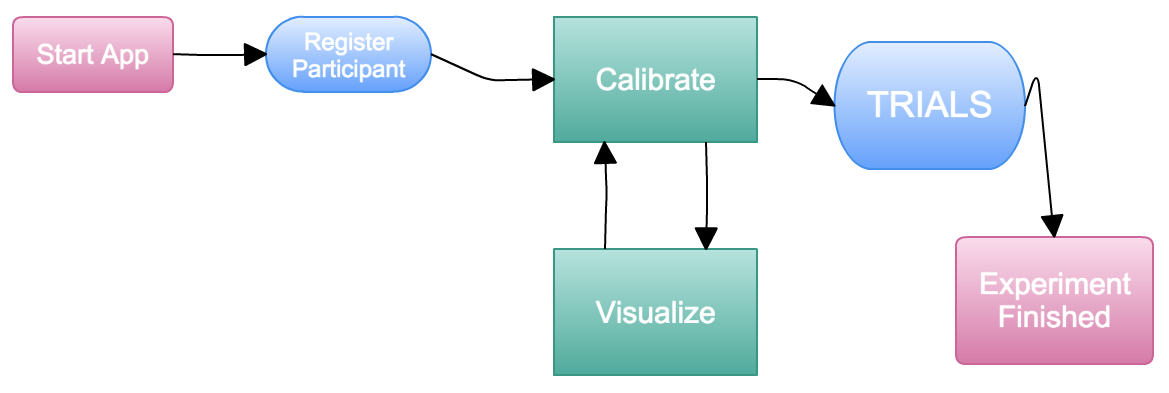
\includegraphics[width=\textwidth]{figures/FFBasicFlow.png}
\caption{Fat Finger - Abstract Flowchart of Basic Modules}
\label{fig:FFBasicFlow}
\end{figure}


%%%%%%%%%%%%%%%%%%%%%%%%%%%%%
%%%%%%%%%%%%%%%%%%%%%%%%%%%%%
%%%%%%%%%%%%%%%%%%%%%%%%%%%%%
%%%%%%%%%%%%%%%%%%%%%%%%%%%%%
%%%%%%%%%%%%%%%%%%%%%%%%%%%%%
%%%%%%%%%%%%%%%%%%%%%%%%%%%%%
\subsection{Basic Design of a Trial}
Each Trial has one basic design and interface. Our target was to find the most obvious and physical way to be able to present all the aspects we wanted, on screen. I ended up on using the design, illustrated in Figure \ref{fig:FFBasicTrialInterface}. The challenging part was in finding a competitive alternative to the simple bar design. The basic usage scenario is:

\emph{The user should move his finger, in a way to alternate the contact area between the screen and his finger. There should be an indicator that will give him feedback. He should know the amount of pressure his is applying to the screen, through a visual representation.}



 \begin{figure}[H]
\centering
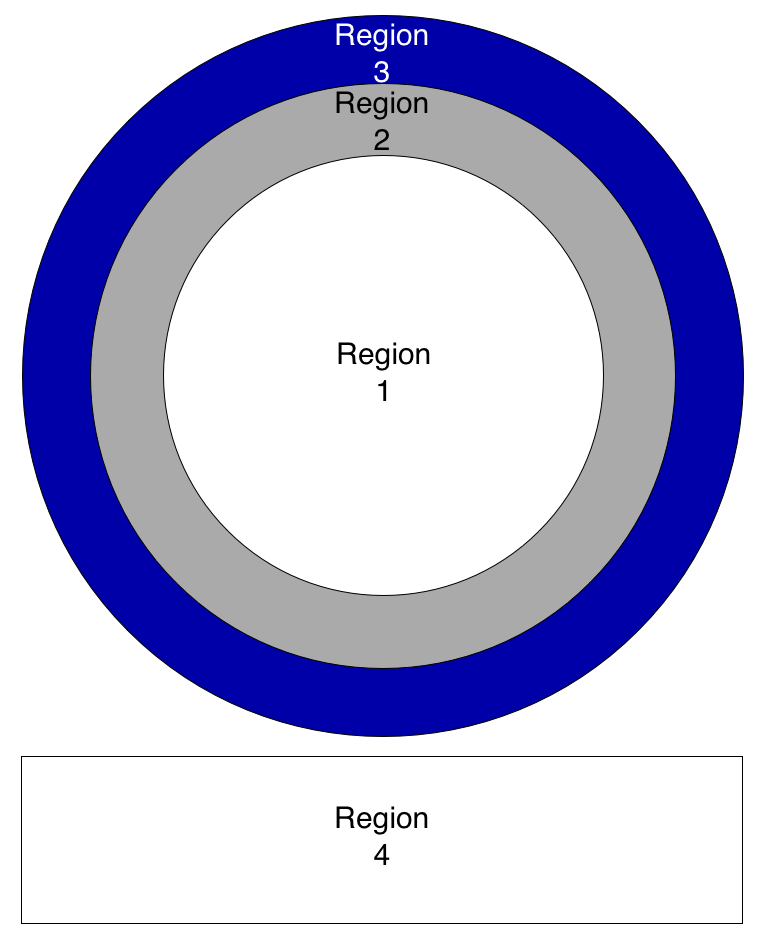
\includegraphics[scale=0.3]{figures/FFBasicTrialInterface.png}
\caption{Fat Finger - Basic Trial Interface}
\label{fig:FFBasicTrialInterface}
\end{figure}

In Figure \ref{fig:FFBasicTrialInterface} we can observe that our interface has 4 regions and all of them are placed on an iPad screen. It is obvious that the whole interface is based on overlapping circles with common center. Table \ref{tab:ffRegions} illustrates the correspondence between Numbers and regions.

\begin{table}[H]
\centering
\begin{tabular}{l || l }
Region No & Description \\
\hline
1 &  Non interactive region. Is placed there, simply in terms of design.\\
2 &  Red coloured targets are placed here.\\
3 &  FeedBack region.\\
4 &  Touch Region. Touch is enabled everywhere though.
\end{tabular}
\caption{Fat Finger - Basic Interface Regions}
\label{tab:ffRegions}
\end{table}

To better assimilate this design lets use a driving example. \emph{Imagine that there is a bar (similar to a progress bar), which is empty when we are barely touching the screen and full when we apply full pressure on the screen. Moreover in each trial, our mission is to achieve a specific level of filling it (e.g. 40\%). Since the bar depicts the movement of our finger, this can be achieved by alternating the area covered by our finger}. 

Now we are ready to move to the next level. Instead of familiarizing with this simple and purely designed idea, I decided to use the circle as the fundamental design shape. Region 3 (Table \ref{tab:ffRegions}) will be alternated while the participant is moving his finger, so as to perfectly map his movement. Therefore, we will have a partially filled circle for the different contact areas (Figure \ref{fig:FFPartlyFilled}).

 \begin{figure}[H]
\centering
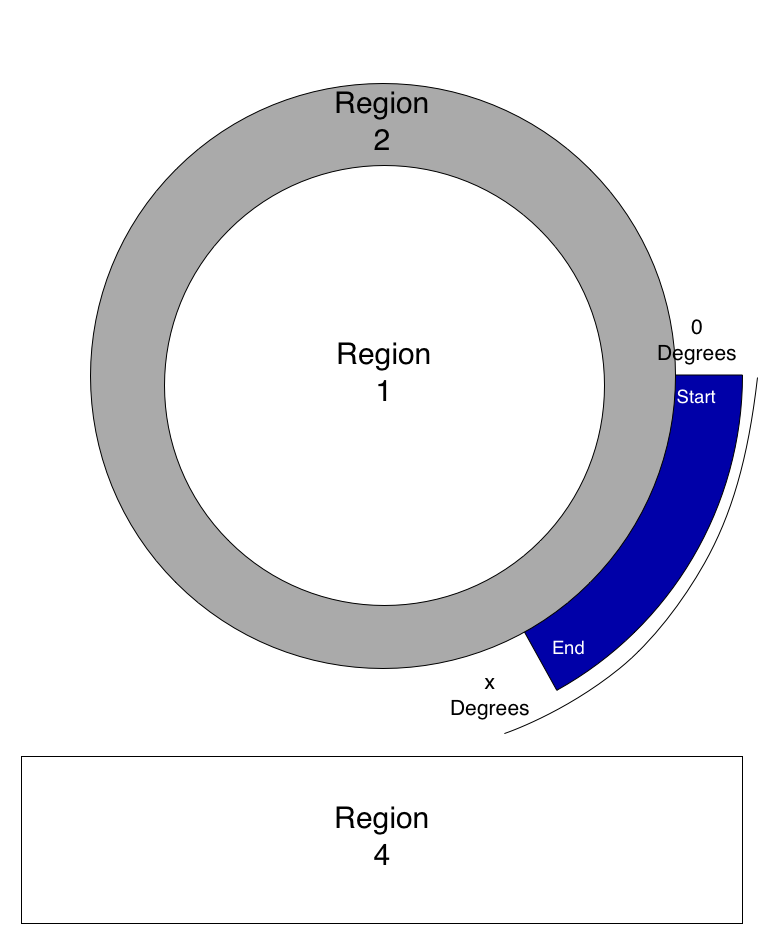
\includegraphics[scale=0.3]{figures/FFPartlyFilled.png}
\caption{Fat Finger - Basic interface during operation}
\label{fig:FFPartlyFilled}
\end{figure}

From Figure \ref{fig:FFPartlyFilled} we can point out many significant characteristics for our design. The starting point of measurement is x-positive axis, and degrees grow with a clockwise orientation. Thus when the contact area is minimum $x=0$, when maximum $x=360$ and $0<x<360$ for all other values. Finally there is a linear correspondence between contact size and degrees $x$, which is calculated through the type: $x = \frac{currentSize - minSize}{maxSize - minSize} * 360$, in degrees.













%%%%%%%%%%%%%%%%%%%%%%%%%%%%%
%%%%%%%%%%%%%%%%%%%%%%%%%%%%%
%%%%%%%%%%%%%%%%%%%%%%%%%%%%%
%%%%%%%%%%%%%%%%%%%%%%%%%%%%%
%%%%%%%%%%%%%%%%%%%%%%%%%%%%%
%%%%%%%%%%%%%%%%%%%%%%%%%%%%%
\section{Trial Categories}

% This section is devoted to present the different Trial categories that are encountered on Fat Finger.
Fat Finger consist of four (4) Trial categories. Those 4 categories are based on the values of 2 binary variables \textbf{TARGET \& FEEDBACK}. The values of this variables can be:
\begin{itemize}
	\item \textbf{TARGET} = \textbf{DISCRETE} or \textbf{CONTINUOUS}
	\item \textbf{FEEDBACK} = be \textbf{FEEDBACK} or \textbf{NO FEEDBACK}
\end{itemize}

Producing all possible combinations of values from TARGET and FEEDBACK we end up having the 4 types we have already mentioned. All possible trials one can encountered belong to one of the those types, which are:


\begin{table}[H]
\centering
\begin{tabular}{l || l | l}
Targeting & Feedback & No Feedback \\
\hline \hline
Discrete & Feedback \& Discrete &  No Feedback \& Discrete\\
Continuous & Feedback \& Continuous & No Feedback \& Continuous
\end{tabular}
\caption{Fat Finger - Trial Categories}
\label{tab:ffTrialCateg}
\end{table}

During the experiment, those 4 types (Table \ref{tab:ffTrialCateg}) will occur multiple times with different variable difficulties. Difficulty can be defined as \emph{"The combination of the position and the size - width of the target"}. The smaller the target the more difficult one trial is. To be able to measure the difficulty of each Trial we use a new variable \textbf{N} which indicates how many buckets each trial has. So First we need to define what a bucket is.

\emph{Bucket is a part of the targets region (Region 2 in Figure \ref{fig:FFBasicTrialInterface}).The target region can be divided in N equal parts. Each of those parts is called Bucket. For example if $N=2$ then the first bucket is the "down" semicircle of the target region ($0-180$ degrees), and the second is the "upper" one ($180-360$ degrees)}

\textbf{N} varies inversely as the value of \textbf{Buckets}. In an inverse variation, the values of the two variables change in an opposite manner - as one value decreases, the other increases. Therefore, as N increases, the range of each bucket decreases. Moreover the ranges of all buckets should add up to 360 degrees. 

At this point, the values for the two basic variables \textbf{TARGET} and \textbf{FEEDBACK} will be thoroughly analyzed.



%%%%%%%%%%%%%%%%%%%%%%%%%%%%%%%%%%%%
%%%%%%%%%%%%%%%%%%%%%%%%%%%%%%%%%%%% 
%% Explain the value of each variable

\begin{itemize}
	\item \textbf{Discrete}. This only relates to Region 2 (Figure \ref{fig:FFBasicTrialInterface}), so the formatting of the targets. In this type, targets are discrete, meaning that Region 2 is divided in N buckets, but only one of them is activated. The activated bucket is coloured in red and acts as the target for this trial. All other inactive buckets are coloured in Gray. 

	\item \textbf{Continuous}. This also relates to Region 2 (Figure \ref{fig:FFBasicTrialInterface}) exclusively. In this type, Region 2 is not divided into buckets, at least visible. We think in term of targets, but we do not present them graphically. The target is just one small red line (a bucket with 1 degree range). However it might have been impossible for the user to select such a tiny target, so we offer an offset area which is delimited with two yellow lines. The position of the target is not random. As I mentioned before, we still think in term of buckets. But instead of considering the whole bucket as a target, we just randomly select a small region inside that bucket, and draw the red line there. Thus, we have the same amount of Trials as in the Discrete type.

	\item \textbf{Feedback} is related with Region 3 (Figure \ref{fig:FFBasicTrialInterface}). In this type, Region 3 is visible, meaning that we have continuous feedback while we are moving our finger. In order to select a target the user has to keep the edge of the blue line (Region 3) inside the red bucket for at least one second. Then a short sound confirms the selection and the trial is dismissed. Summarizing, the mission is: 

	\emph{Keep the edge of the blue "line" inside the red target for one second}.

	\item \textbf{No FeedBack} is also related with region 3 (Figure \ref{fig:FFBasicTrialInterface}). In this type, Region 3 is now invisible. Therefore we do not have feedback indicator while we are alternating the contact area between our finger and the screen. Thus we need to memorize the movement and be able to predict the position of the edge of the "blue" region. To confirm selection, user has to lift his finger from the screen. The software will then choose the last contact area size,  before the lift as the one the user implied. As a consequence we can only lift the finger one time. We are not allowed to perform retouches, because on the first lift, target selection will be performed. 

	It should also be mentioned that, in this type of trials, we are not forced to hit the target successfully. We just make a prediction and then lift our hand. Our input will be recorded and then displayed to us through a graphical Confirmation Interface.  Summarizing, in this type, our mission is:

	\emph{Touch the screen, alternate the contact area and make a prediction on where the blue line should be to hit the target, lift the finger when you are on the preferred contact size, and finally observe the outcome - feedback}.
\end{itemize}

We have now explained and introduced all the necessary background, and we are ready to present the Interface of the 4 categories of trials as stated in Table \ref{tab:ffTrialCateg}.

%%%%%%%%%%%%%%%%%%%%%
%%%%%%%%%%%%%%%%%%%%%
%%%%%%%%%%%%%%%%%%%%%

\subsection{Feedback \& Discrete Targeting}


In this type of trials, we can understand that the targets will be discrete and there will also be feedback on our input. Figure \ref{fig:FD} presents the interface of this type. As we can see both Region 2 and 3 (Figure \ref{fig:FFBasicTrialInterface}) exist. Since we have \emph{Discrete} targets, Region 2 is separated in $n$ buckets, all with equal size. The target is the one coloured in red, and all others are inactive and coloured in gray. On the other hand, \emph{Feedback} keyword is mentioned too, which means that the blue circle (Region 3) exists. The movement of the blue region corresponds to the movement of our hand. To accomplish this trial, the participant needs to keep the moving edge of the blue region inside the range of the target (red bucket), for at least 1 second. Then a confirmation sound is being played, which proceed us to the next trial.

\begin{figure}[H]
\centering
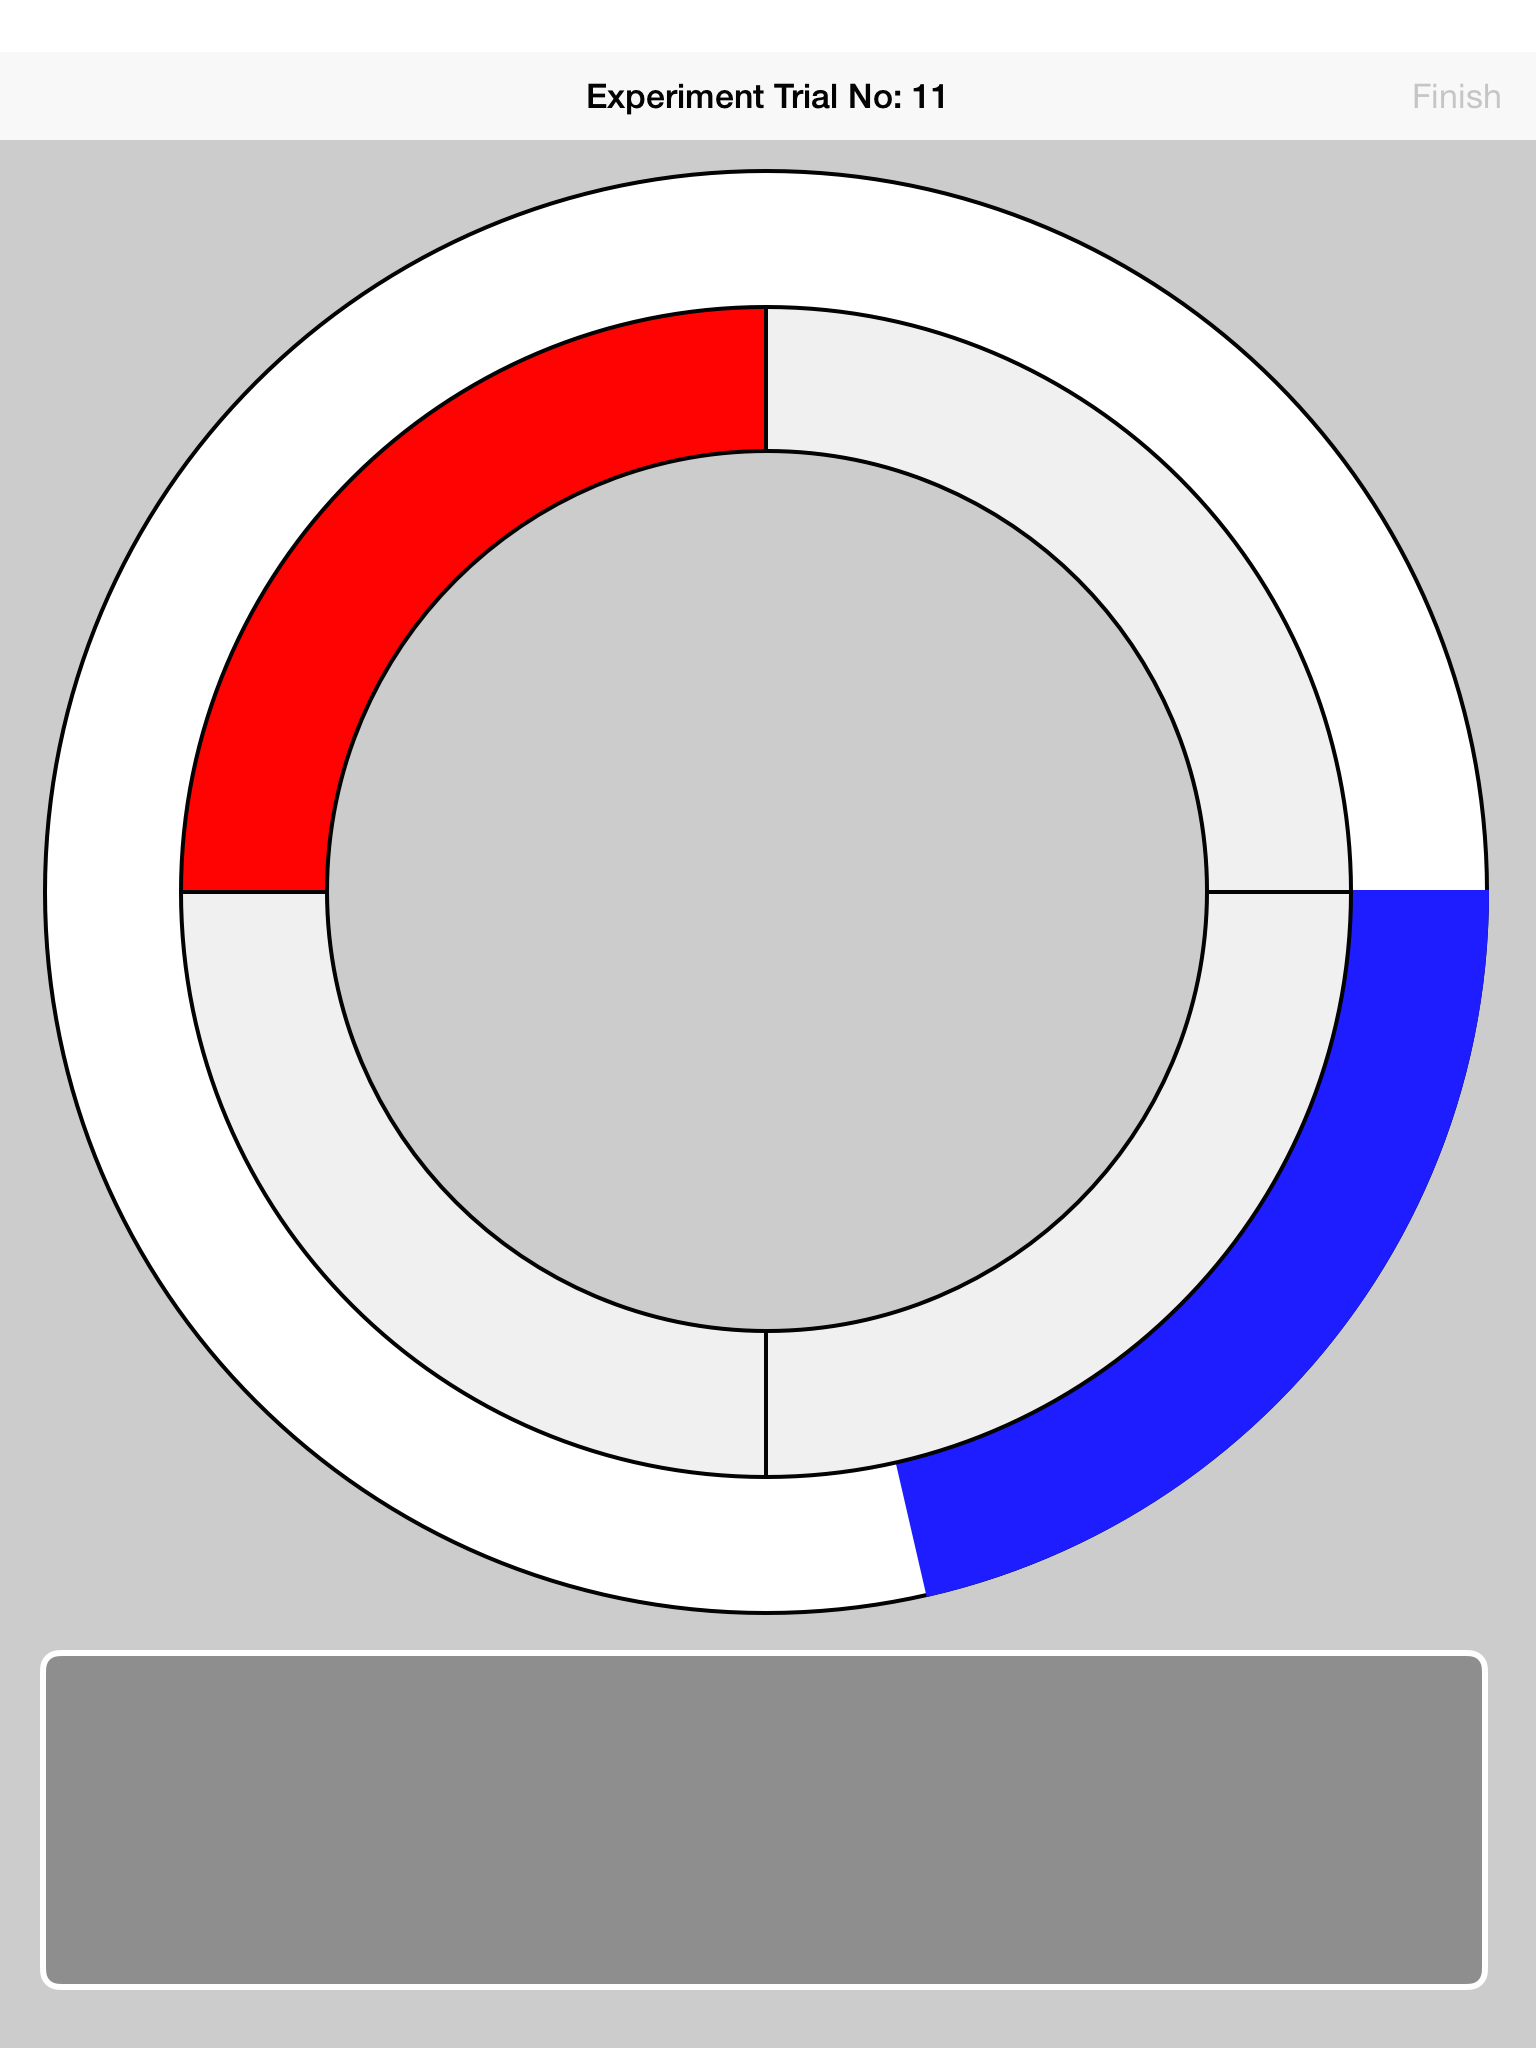
\includegraphics[scale=0.07]{figures/FD.png}
\caption{Feedback \& Discrete Targeting Interface}
\label{fig:FD}
\end{figure}


%%%%%%%%%%%%%%%%%%%%%
%%%%%%%%%%%%%%%%%%%%%
%%%%%%%%%%%%%%%%%%%%%

\subsection{Feedback \& Continuous Targeting}

In this occasion, we are still provided with feedback on our input, but the target will now be of type Continuous. Figure \ref{fig:FND} presents the interface of this category. \emph{Continuous} targets mean that only one thin red line exist in Region 2 (Figure \ref{fig:FFBasicTrialInterface}). While the position of the target is related with buckets, the actual buckets are just invisible. As we previously mentioned, the red line is randomly positioned within one of the N buckets. The two yellow lines, surrounding the red one are the offset limits and their distance is the offset range.  User can confirm a target by staying inside that range, however he is instructed to target as close and accurate to the target as possible. Finally, \emph{Feedback} keyword specifies that Region 3 exists. The process for confirming the selection of a target, is to keep the moving edge of the blue region inside the range of the target (yellow lines), for at least 1 second.

\begin{figure}[H]
\centering
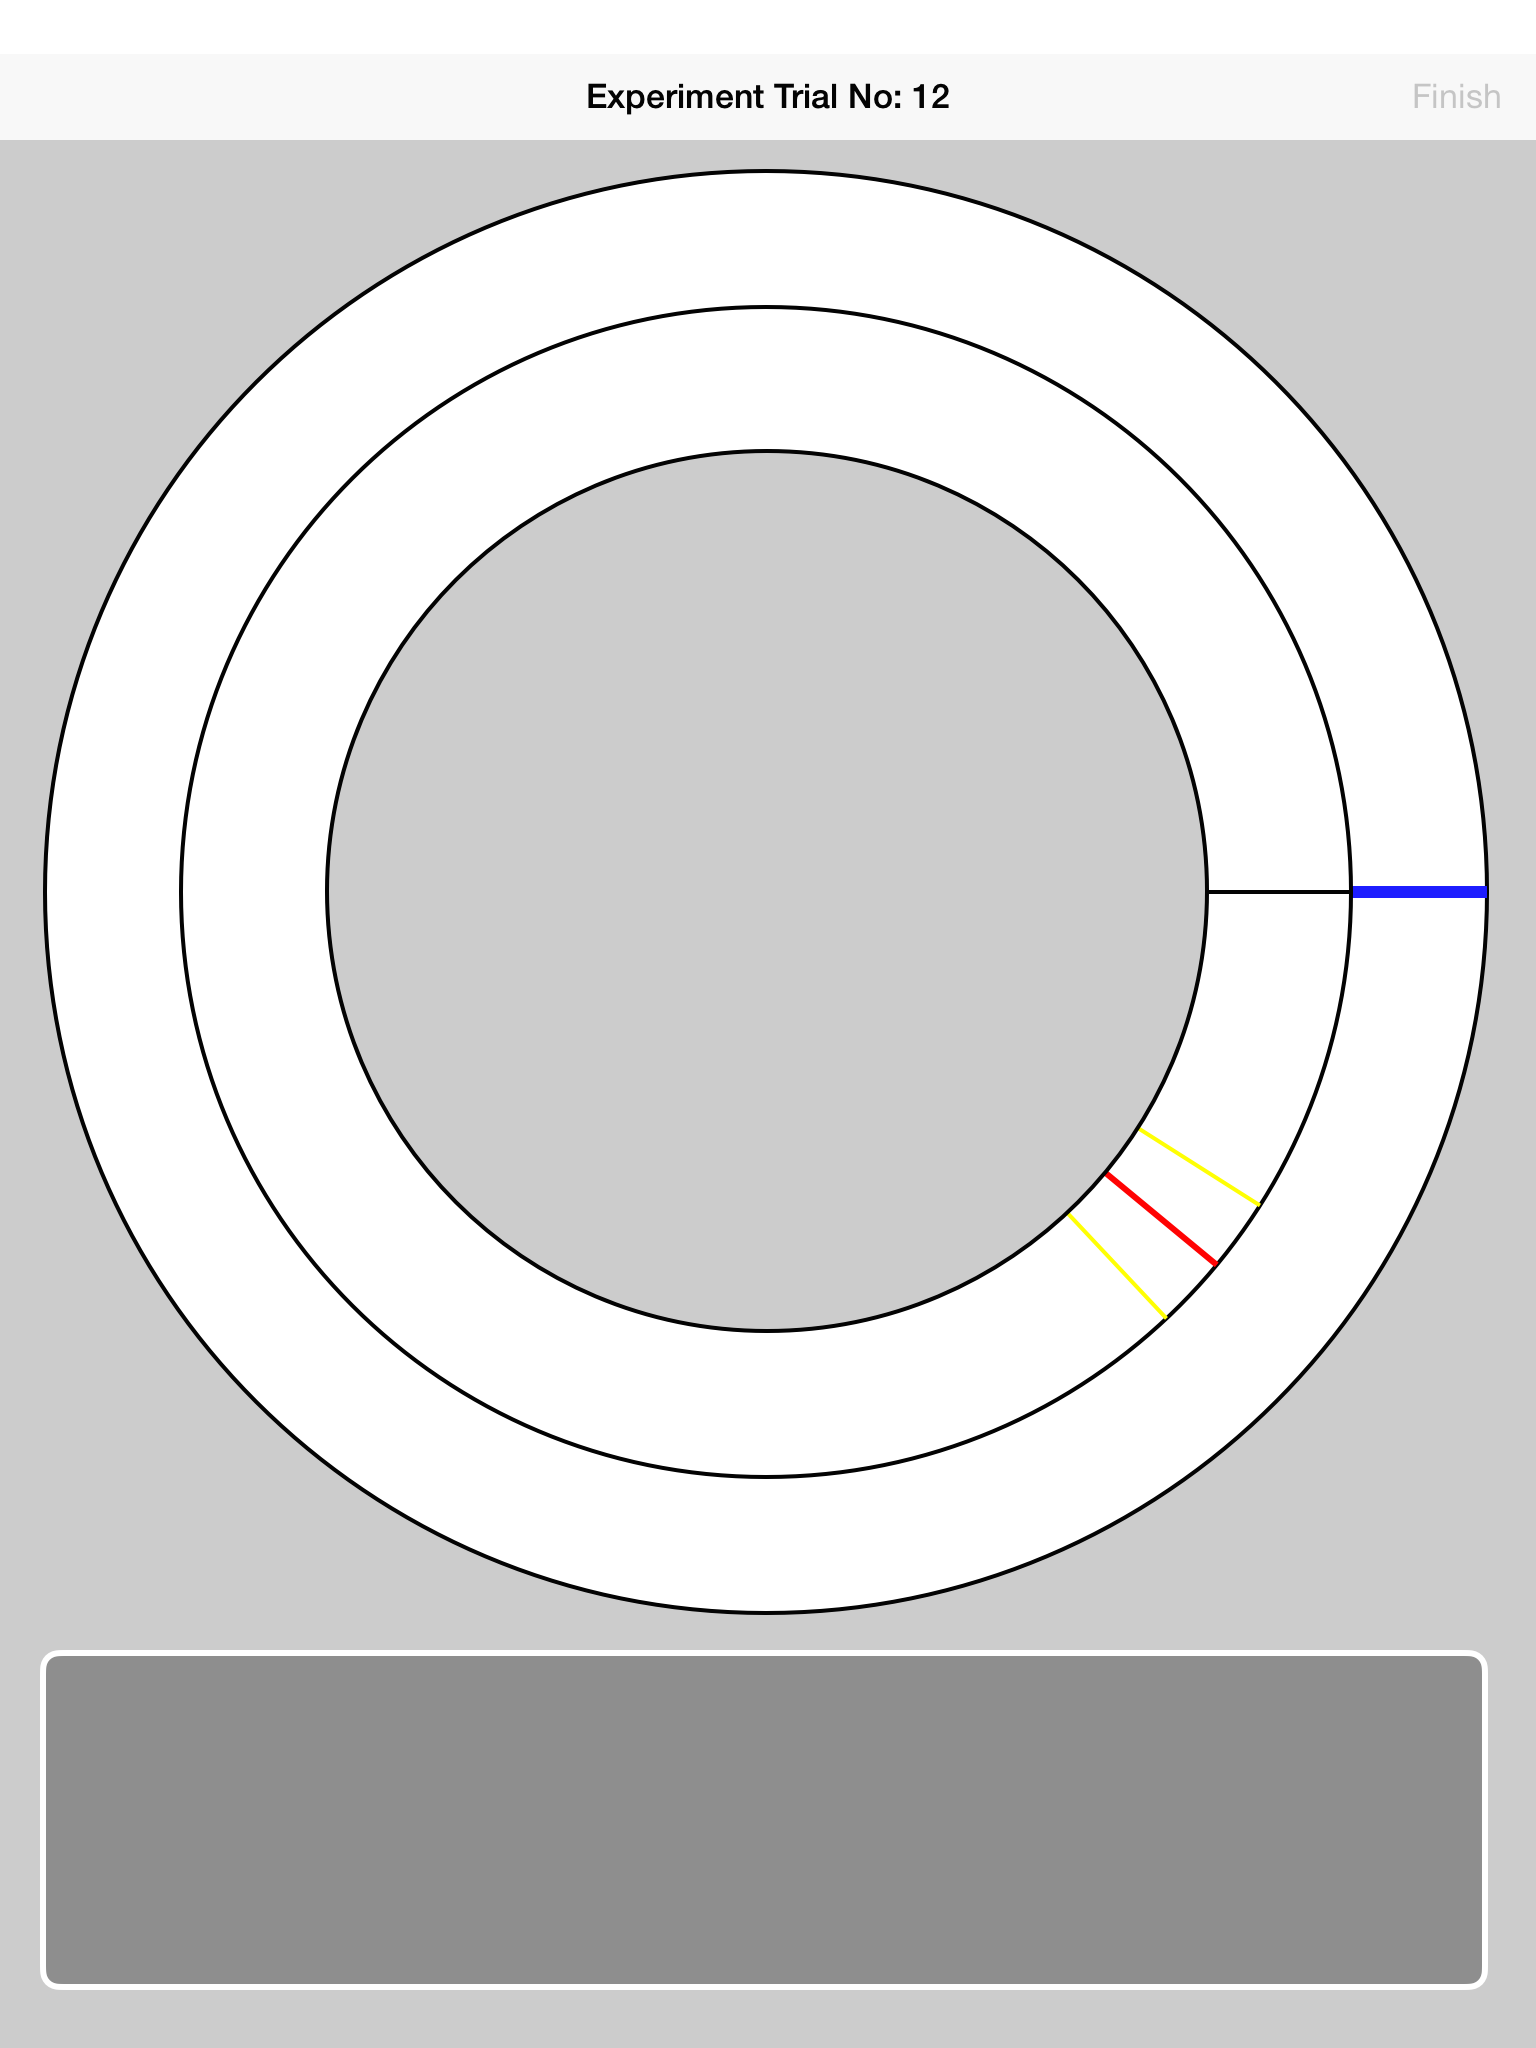
\includegraphics[scale=0.07]{figures/FND.png}
\caption{Feedback \& Continuous Targeting Interface}
\label{fig:FND}
\end{figure}

%%%%%%%%%%%%%%%%%%%%%
%%%%%%%%%%%%%%%%%%%%%
%%%%%%%%%%%%%%%%%%%%%
\subsection{No Feedback \& Discrete Targeting}

The rules for \emph{Discrete} targets apply and here. Thus, Region 2 (Figure \ref{fig:FFBasicTrialInterface}) is separated in $N$ buckets, all with equal size. Variable $N$ mostly specifies the difficulty of the trials. The target is the one coloured in red, and all others are inactive and coloured in gray. This category differs from the aforementioned because it is of type \emph{No Feedback}. That means that Region 3 (Figure \ref{fig:FFBasicTrialInterface}) does not exist. So, in the beginning we encounter the interface illustrated in Figure \ref{fig:NFD}. Our task  is to \textbf{a}) touch the screen, \textbf{b}) predict the contact area needed to select the target and \textbf{c}), confirm selection by lifting the finger form the screen. After confirming selection, we face the \textbf{Confirming Interface} shown in Figure \ref{fig:NFDConfirm}, in which we can observe our performance in the trials. Did we hit that target or not? This input can be used as a learning parameter which will help us to improve our performance as we move through the trials.

\begin{figure}[H]
\centering
\begin{subfigure}[b]{0.3\textwidth}
	\centering
	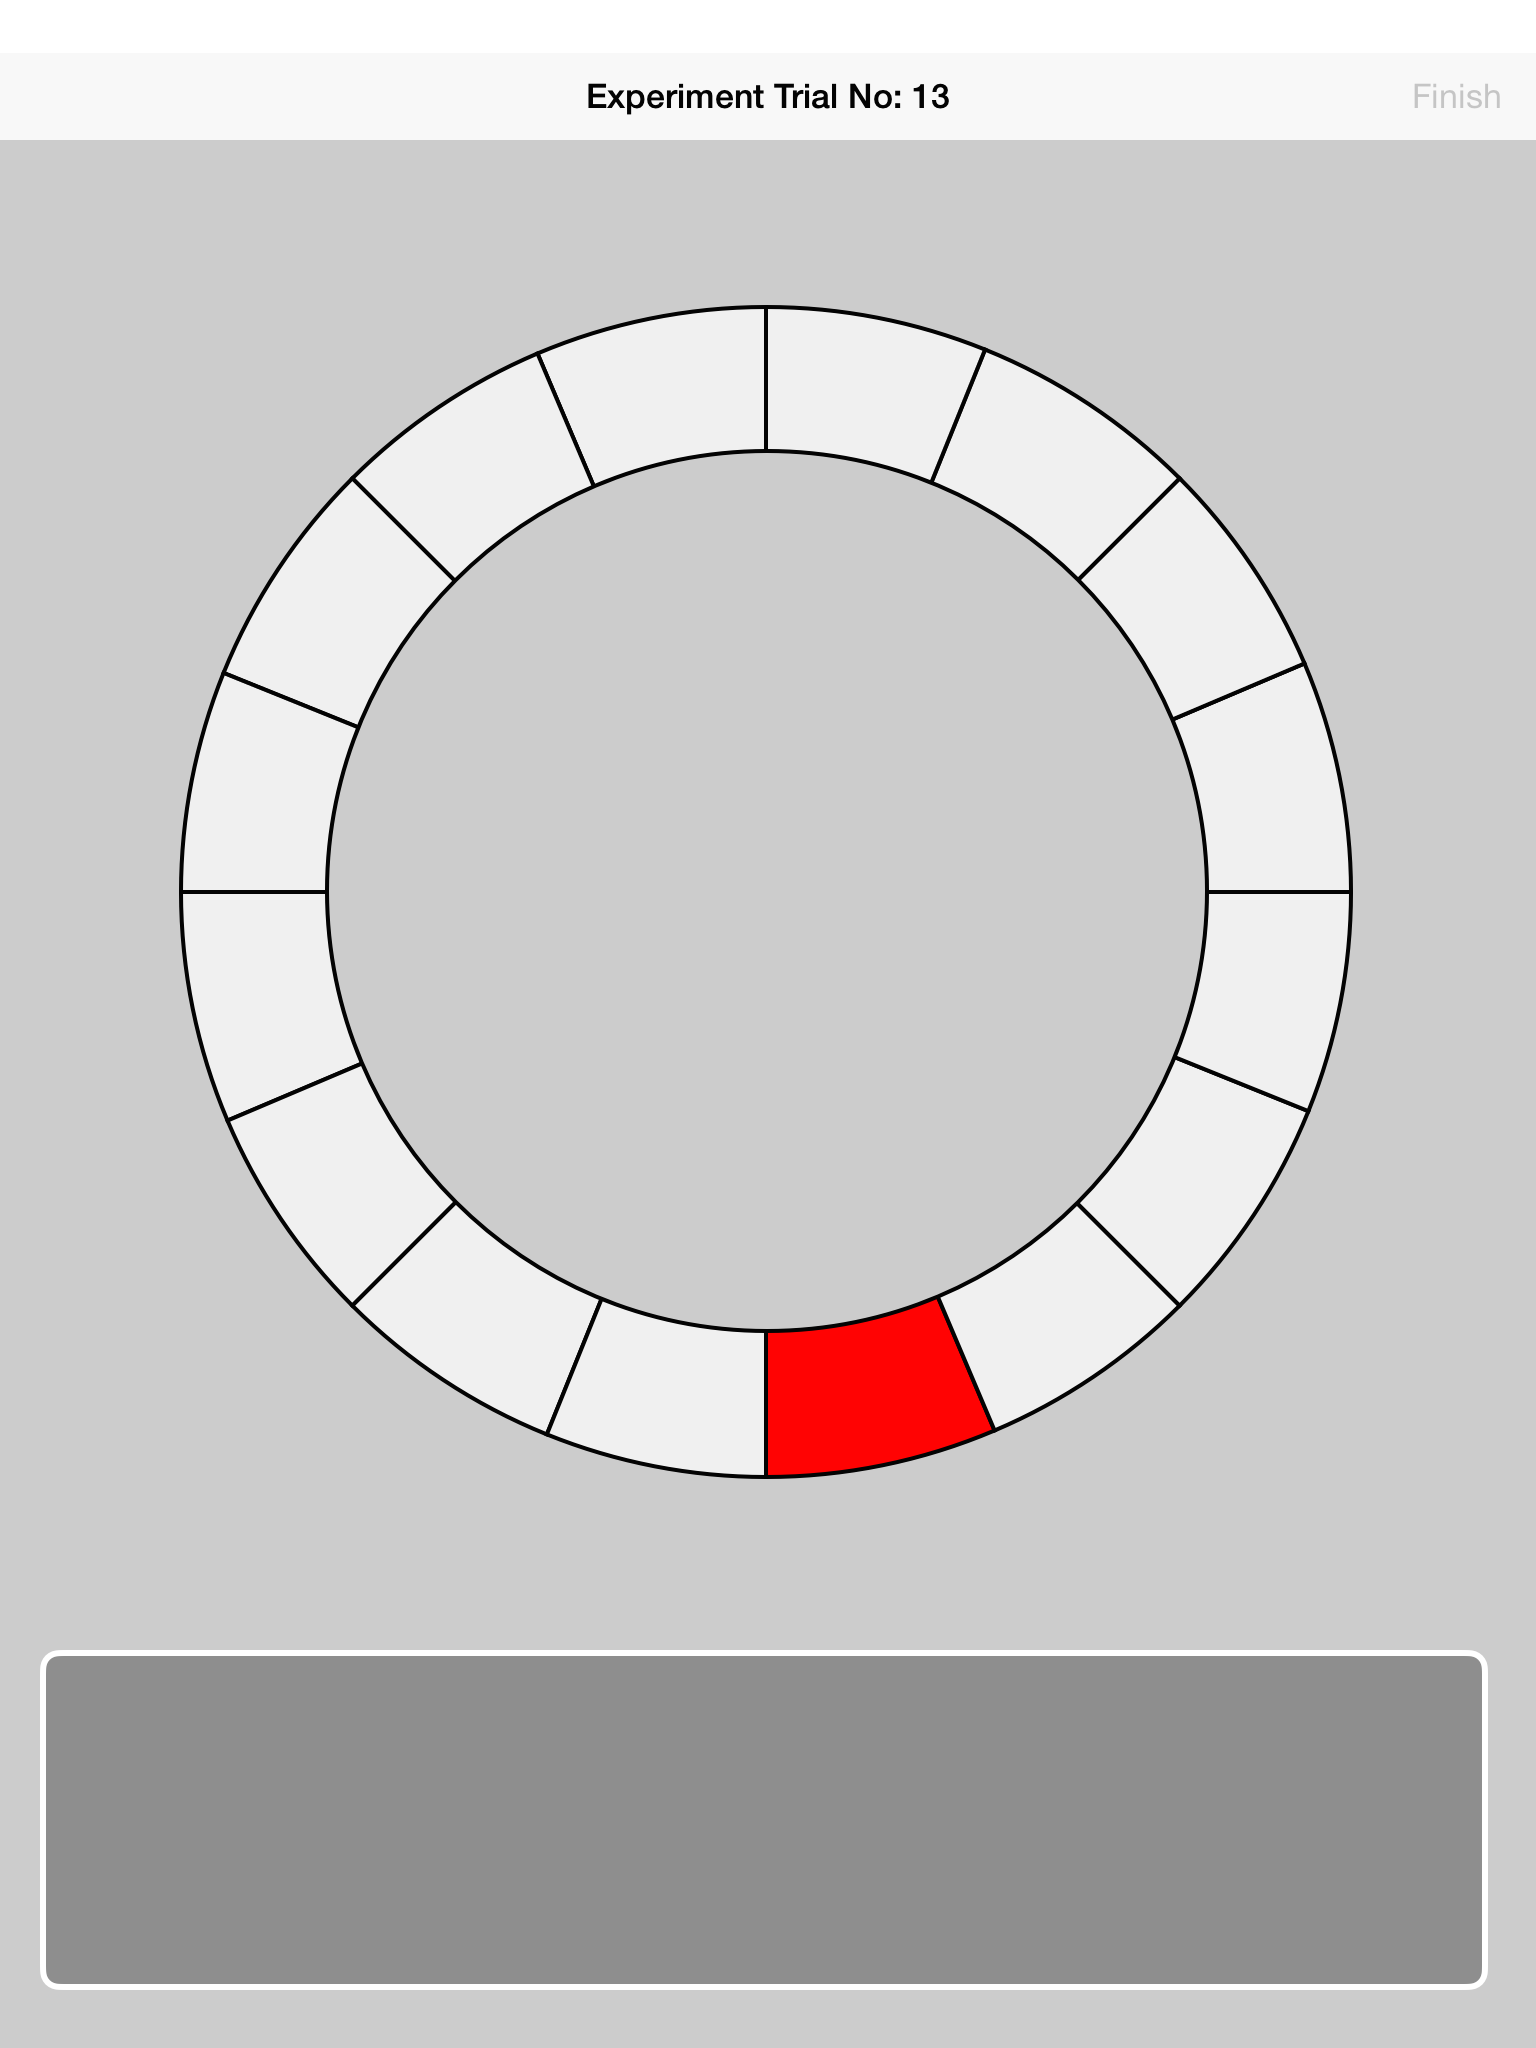
\includegraphics[width=\textwidth]{figures/NFD.png}
	\caption{Targeting Interface}
	\label{fig:NFD}
\end{subfigure}
\hfill
\begin{subfigure}[b]{0.3\textwidth}
	\centering
	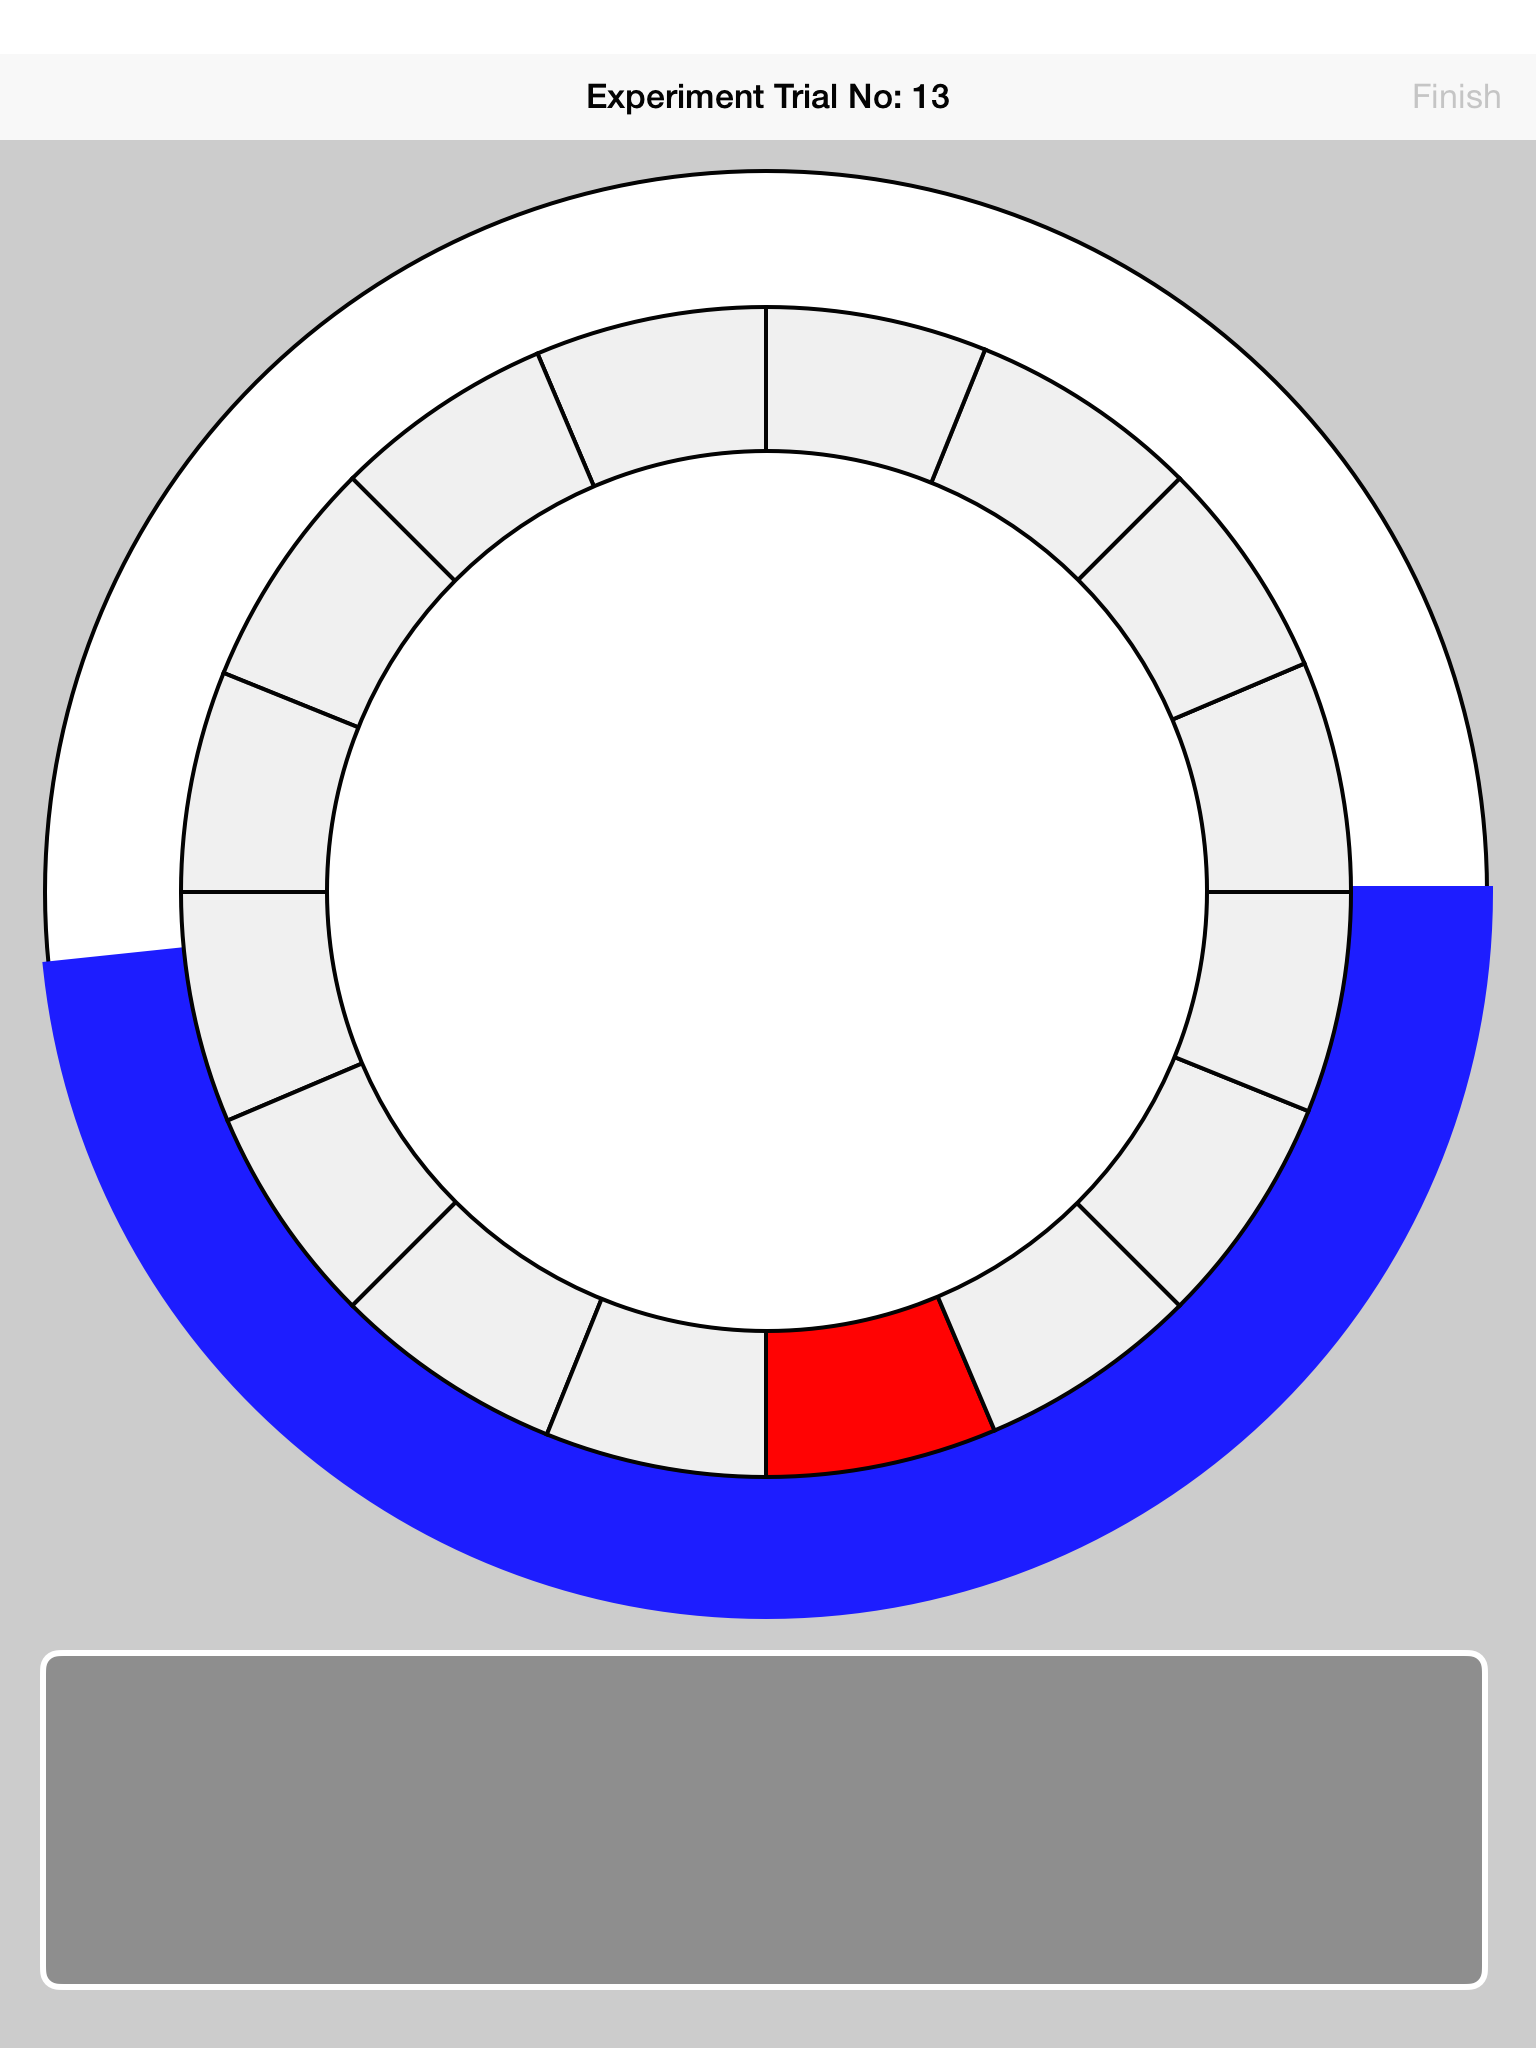
\includegraphics[width=\textwidth]{figures/NFDConfirm.png}
	\caption{Confirmation Interface}
	\label{fig:NFDConfirm}
\end{subfigure}
\caption{No Feedback \& Discrete Targeting and Confirmation Interface}
\label{fig:NFDGraph}
\end{figure}

%%%%%%%%%%%%%%%%%%%%%
%%%%%%%%%%%%%%%%%%%%%
%%%%%%%%%%%%%%%%%%%%%
\subsection{No Feedback \& Continuous Targeting}

\begin{figure}[H]
\centering
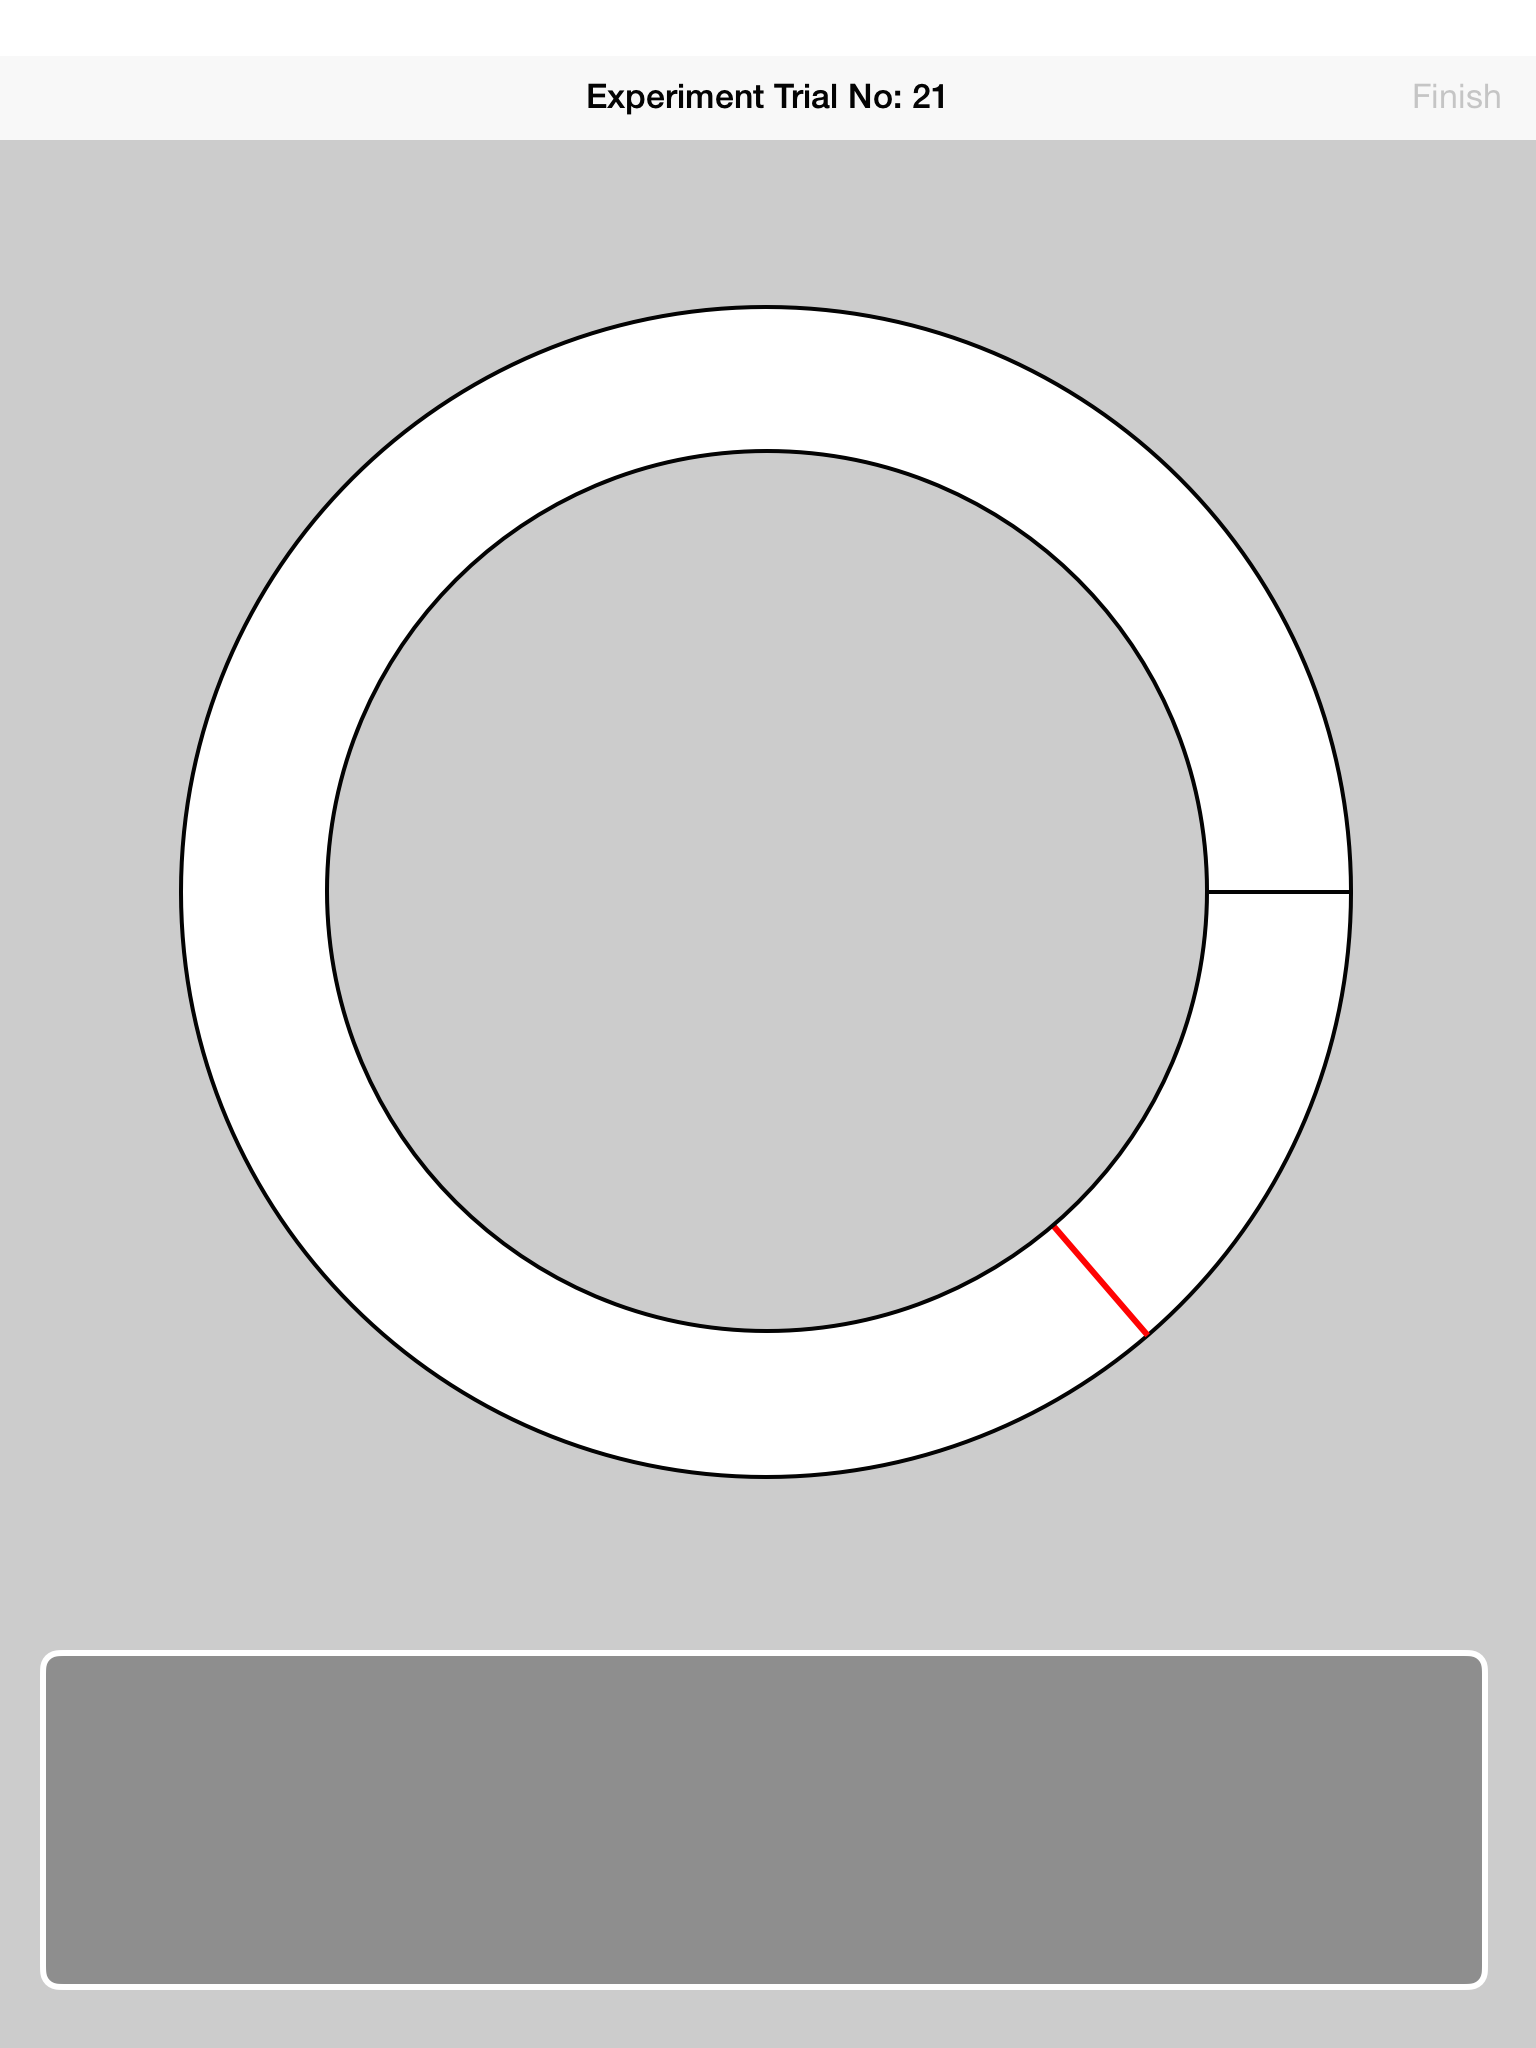
\includegraphics[scale=0.07]{figures/NFND.png}
\caption{No Feedback \& Continuous Targeting Interface}
\label{fig:NFND}
\end{figure}

Figure \ref{fig:NFND} presents the interface of the \emph{No Feedback \& Continuous Targeting} category. Targets are \emph{Continuous}, meaning that only one thin red line exist in Region 2 (Figure \ref{fig:FFBasicTrialInterface}). The two yellow lines, surrounding the red one still exist. They represent the offset limits and their distance is the offset range. It also of type \emph{No Feedback}. Thus, Region 3 (Figure \ref{fig:FFBasicTrialInterface}) does not exist. Our task is again to \textbf{a}) touch the screen, \textbf{b}) predict the contact area needed to select the target and \textbf{c}), confirm selection by lifting the finger form the screen. After confirming selection, we once more face the \textbf{Confirming Interface} shown in Figure \ref{fig:NFDConfirm}, in which we can observe our performance in the trials. 



%%%%%%%%%%%%%%%%%%%%%%%%%%%%%
%%%%%%%%%%%%%%%%%%%%%%%%%%%%%
%%%%%%%%%%%%%%%%%%%%%%%%%%%%%
%%%%%%%%%%%%%%%%%%%%%%%%%%%%%
%%%%%%%%%%%%%%%%%%%%%%%%%%%%%
%%%%%%%%%%%%%%%%%%%%%%%%%%%%%
\section{Final Sequence of Trials}
\label{sec:FinalSequenceofTrials}

% Explain   the   repetitions,   randomization,   and   generally   how   the   sequence   of each experiment is calculated.

Thus far we have explained all the main characteristics of our experiment. Now we should focus on the final sequence of the trials and the whole structure of the experiment. In this experiment we want to investigate 7 different N's, or bucket sizes. N can have the following values:

N = [2,3,4,6,8,12,16]

For each n we have the same amount of related targets. For instance if $N=2$, then we have two available targets, one for each bucket. If $N=4$, the we have 4 possible targets, etc.
As a result for all the above mentioned values for N we can gave the following number of possible targets:

$2(N=2)+3(N=3)+4(N=4)+6(N=6)+8(N=8)+12(N=12)+16(N=16) = 51 targets$

Then we have 4 different types of Trials: Feedback \& Discrete, No Feedback \& Discrete, Feedback \& Continuous, No Feedback \& Continuous.

For each of the above categories we conduct all the aforementioned targets. So the total number of Trials is:
$51*4 = 204$. Furthermore we need to randomize their order just to make sure that it will not have any effect in our study. After the randomization takes place we say that we have 1 \textbf{Repetition} of the Trials. Figure \ref{fig:ffRepetition} graphically illustrates this procedure.


\begin{figure}[H]
\centering
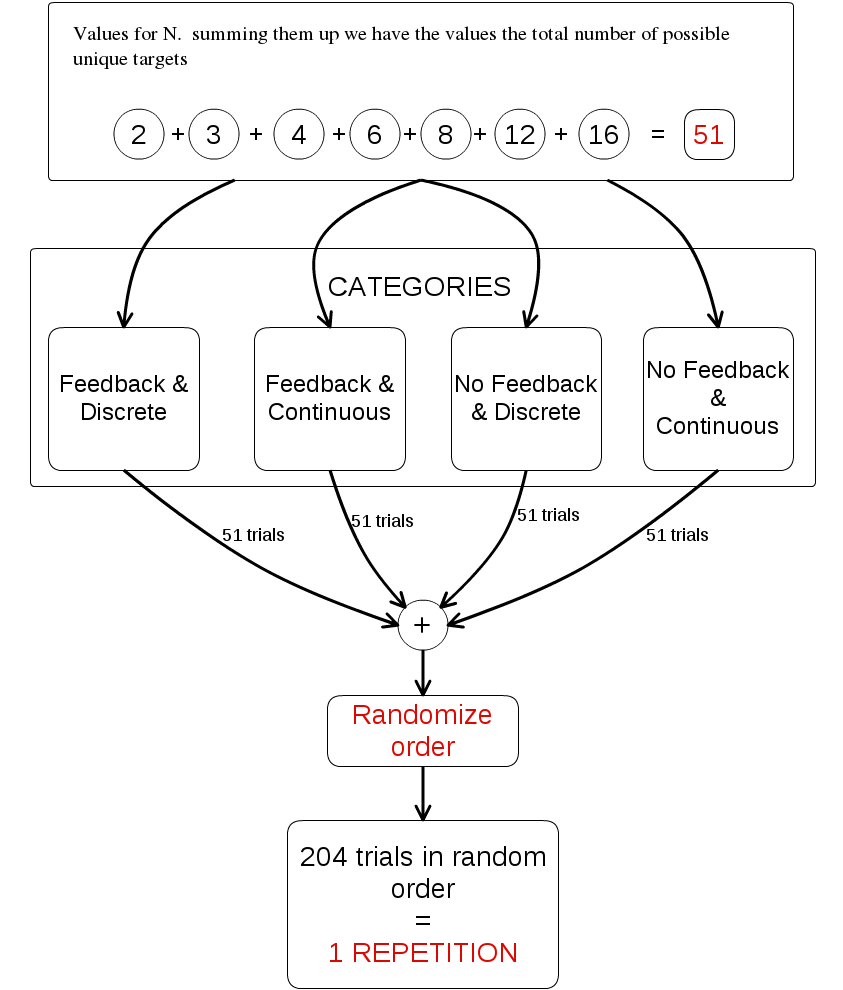
\includegraphics[width=0.6\textwidth]{figures/repetition.png}
\caption{Repetition Calculation}
\label{fig:ffRepetition}
\end{figure}


This experiment contains 3 repetitions of those trials and not only 1. So in Total we will have $203*3repetitions = 612 trials$. We chose to have 3 Repetitions for the following 2 main reasons. 

\begin{itemize}
	\item There is no Warm up session for this experiment. Instead of having separate trials to prepare the users for this experiment we chose to combine the Learning phase with the 1st repetition of the Trials. That way we can observe the Learning effect taking place. 

	\item The experiment should last enough so as to give users the time to absorb the information given, familiarize with the environment and the technique and also explore whether side effects as distraction of attention and fatigue have an impact on the performance of the users.
\end{itemize}

Figure \ref{fig:ffRepetition} graphically illustrates how the repetitions are combined together. It also gives an overview of the work-flow of Fat Finger.

\begin{figure}[H]
\centering
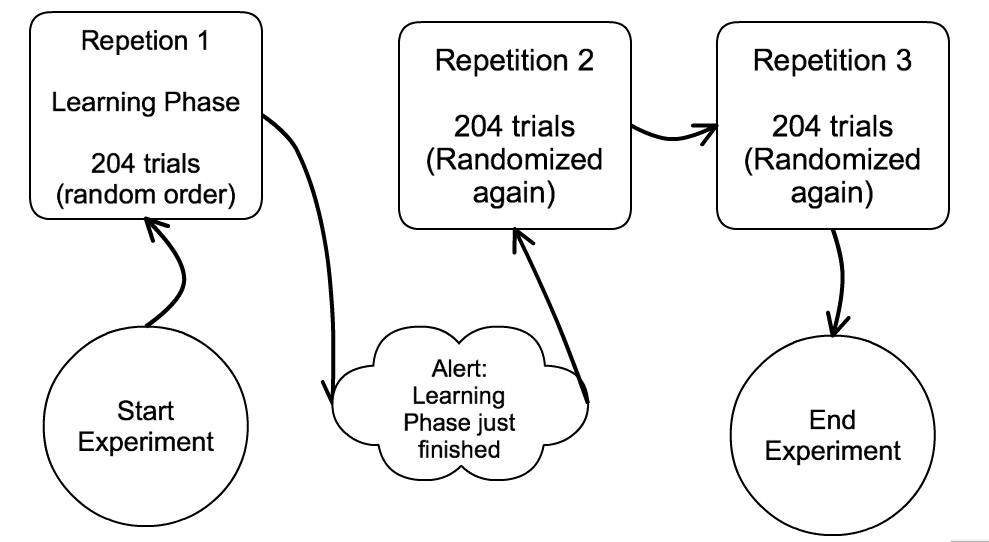
\includegraphics[width=0.6\textwidth]{figures/ffRepetitions.png}
\caption{Fat finger - Generalized experiment flow of repetitions}
\label{fig:ffRepetitions}
\end{figure}


%%%%%%%%%%%%%%%%%%%%%%%%%%%%%
%%%%%%%%%%%%%%%%%%%%%%%%%%%%%
%%%%%%%%%%%%%%%%%%%%%%%%%%%%%
%%%%%%%%%%%%%%%%%%%%%%%%%%%%%
%%%%%%%%%%%%%%%%%%%%%%%%%%%%%
%%%%%%%%%%%%%%%%%%%%%%%%%%%%%
\section{Data Manipulation}

Data Monitoring and Exporting are of significant importance when we have to deal with the accomplishment of an experiment. When performing a user study you need to decide which parameters you are going to monitor, and to find a way to measure them. Code-wise, you need to implement a software that is able to calculate all the metrics you want to observe, and then store them somewhere consistently. After the experiment is finished, it is truly crucial to be able to export those data from the place they are stored into a common format that is accessible from another program. Summarizing we have a three step process when we conduct an experiment. 

\begin{enumerate}
	\item Decide which parameters to measure.
	\item Store the observed values in a consistent database.
	\item Export the data to appropriate format (.xls, .csv, etc.)
\end{enumerate}

Our approach for the first two points is analyzed on section \ref{sec:monitoring}, while for the latter on section \ref{sec:exporting}.
%%%%%%%%
%%%%%%%%
%%%%%%%%
%%%%%%%%
%%%%%%%%
\subsection{Monitoring}
\label{sec:monitoring}

Table \ref{tab:ffUniData} presents the basic parameters we measure that are common for all types of trials. The first column contains the name of the corresponding variable, the second a short description of its usage, and on the third we can observe which is the field of values for each variable.

%%%%
%% Universal Parameters
%%%%

\begin{table}[H]
\centering
\begin{tabular}{l || l || l}
Name & Description & Field of Values\\
\hline \hline
\textbf{trialID} & Incremental id of this trial & [1, 2, ..., 612] \\
\textbf{typeID} & Id of the type of the trial & [1,2,3,4] \\
\textbf{N} & Total number of Buckets & [2,3,4,6,8,12,16] \\
\textbf{min} & the minimum calibrated radius & $Float > 0$ \\
\textbf{max} & the maximum calibrated radius & $Float > 0$ \\
\textbf{rawInputValue} & Raw Value between Min and Max & Float number \\
\textbf{reEntries} & Number of Target Re-entries & $Decimal >= 0$ \\
\textbf{repetitionID} & Repetition id they belong to & [1,2,3] \\
\textbf{reTouches} & Number of Target Re-Touches & $Decimal >= 0$ \\
\textbf{target} & Which of the buckets was the target  & [1,2,...,n]\\
\textbf{totalTime} & Total time to accomplish the Trial & Float number
\end{tabular}
\caption{Fat Finger - Universal Parameters Monitored}
\label{tab:ffUniData}
\end{table}

Combining the above values, apart form being able to uniquely identify the trials of the experiment, we can also reconstruct the whole experiment. This can be achieved, because we are storing the outcome of each trials, the rawData we collected form the user, the total time, etc. Now, we should further analyse each of those parameters:

\begin{itemize}
	\item \textbf{trialID}. Unique identifier for each trial. Most importantly it specifies the order of appearance of the experiments. The first trial with has id 1, the second 2 etc. 

	\item \textbf{N}. Specifies the number of Buckets. \textbf{N} is an indicator that is related, at least in the Feedback trials, with the difficulty. This study is mainly concerned in specifying an upper limit for the number of identifiable levels in the contact area range. Thus, N is the sorting parameter for being able to distinguish the upper limit for those levels. 
	
	\item \textbf{min}. The minimum value for the PathMajorRadius we collected from the calibration. During the calibration process, user can calibrate his finger as many times as he want. When he proceeds to the experiment, we collect the lastly calibrated values and store them accordingly.
	
	\item \textbf{max}. The same applies here too, except that we are referring to the maximum value of the PathMajorRadius.  
	
	\item \textbf{rawInputValue}. This is the PathMajorRadius value, for the contact area that hit the target. For Feedback trials, it is the last touch input size exactly when the 1 second delay passed. For No feedback, it is the area just before lifting our finger.
	
	\item \textbf{reEntries}. Counts the times we went outside the target region. It starts counting after the initial entry to the target.
	
	\item \textbf{repetitionID}. Identifies in which of the three repetitions this trial belongs to.  
	
	\item \textbf{reTouches}. Counts how many times we lifted our finger off the screen. Of course for \emph{No Feedback} trials this parameter is always zero since we confirm target selection by lifting our finger from the screen.
	
	\item \textbf{target}. Specifies which of the buckets is the target. Thus it can take values from 1 to N.
	
	\item \textbf{totalTime} Total completion time of the trial. The timer fires when the first touch is performed and stops when the confirming sound is being played. As a result \emph{Feedback} trials will have values $>=$ 1 second. This is because one second is the duration  someone has to inside the target region to confirm target selection. On the other hand, on \emph{No feedback} trials, durations are generally shorter.
\end{itemize}



The above parameters are measured for all 4 types of trials. However, all except for \emph{Feedback\& Discrete} required some extra monitoring. \textbf{Feedback \& Continuous} has the following two extra measured parameters that are also presented in Table \ref{tab:ffFNDData}:

\begin{itemize}
	\item \textbf{targetPosition}. Defines the exact position of the Target. In this type, target is represented as a thin red line. The position will always be inside the \textbf{target}-th bucket out of the \textbf{n} in total. However since it is randomly positioned inside this bucket we needed to record, its accurate position. Value monitored is between \textbf{min} and \textbf{max}. To transform the position into circle degrees we can use the type $PositionInDegrees = \frac{targetPosition-min}{max-min}360$.
	\item \textbf{offset} Indicates how far we were from the target. It can be thought as an error rate too. The higher the offset the higher the error we performed on our selection. Positive values mean that we hit somewhere after the target. Negative values mean that we hit before it. Also offset is measured in percentage. If we want to find how many degrees we were off the target then we can just use the type: $DegreesOff = offset*360$
\end{itemize}

%%%%
%% Feedback Continuous Parameters
%%%%

\begin{table}[H]
\centering
\begin{tabular}{l || l || l}
Name & Description & Field of Values \\
\hline \hline
\textbf{targetPosition} & Position of the Target & \textbf{min}$<=$Float$<=$\textbf{max} \\
\textbf{offset} & Distance from target in percentage & float :[-1 to +1] 
\end{tabular}
\caption{Fat Finger - Feedback \& Continuous Targeting additional parameters monitored}
\label{tab:ffFNDData}
\end{table}


\textbf{No Feedback \& Discrete} targeting requires a different set of extra parameters to be measured. Feedback region does not exist in this type, which means that users have to predict where the feedback region is. This type of Trial requires longer learning time. Thus for the initial trials we expect that participants predictions-guessing will not be very accurate. As a result, the error rates / offset will be high. To monitor that we use the following two parameters as shown in Table \ref{tab:ffNFDData}:
\begin{itemize}
	\item \textbf{hitInsideTarget} As it can be inferred form its name, it indicates whether we actually hit inside the Target or outside. 
	\item \textbf{offset} mostly represents the error in percentage over the whole range. In \emph{No Feedback} trials error can be extremely high as there is no limitation that the user can confirm selection, while explicitly being inside the target. Thus positive values mean that the selection was performed at a point after the center of the target, while negative values stand for before.
\end{itemize}


%%%%
%% No Feedback Discrete Parameters
%%%%
\begin{table}[H]
\centering
\begin{tabular}{l || l || l}
Name & Description & Field of Values  \\
\hline \hline
\textbf{offset} & Distance from target in percentage & float :[-1 to +1] \\
\textbf{hitInsideTarget} & Indicates if we successfully hit the Target & True, False
\end{tabular}
\caption{Fat Finger - No Feedback \& Discrete Targeting additional parameters monitored}
\label{tab:ffNFDData}
\end{table}

Finally, in \textbf{No Feedback \& Continuous Targeting} we meet a combination of the extra parameters we have already mentioned. It is thought to be the most tough type of experiment, since we neither have feedback, nor small targets. To better monitor this type we use those extra supplementary parameters, as illustrated in Table \ref{tab:ffNFNDData}. Each of them has been already explained and analyzed in the aforementioned types.


%%%%
%% No Feedback Continuous Parameters
%%%%

\begin{table}[H]
\centering
\begin{tabular}{l || l || l}
Name & Description & Field of Values \\
\hline \hline
\textbf{offset} & Distance from target in percentage & float :[-1 to +1] \\
\textbf{targetPosition} & Position of the Target & \textbf{min}$<=$Float$<=$\textbf{max} \\
\textbf{hitInsideTarget} & Indicates if we successfully hit the Target & True, False
\end{tabular}
\caption{Fat Finger - No Feedback \& Continuous Targeting additional parameters monitored}
\label{tab:ffNFNDData}
\end{table}

%%%%%%%%
%%%%%%%%
%%%%%%%%
%%%%%%%%
%%%%%%%%
\subsection{Exporting}
\label{sec:exporting}

Monitoring the results and saving them into a database was half the way towards the fulfilment of our study. There is a need to export them into a reasonable format so that thy can be imported into a Statical Analysis tool. Fat Finger used Core Data for storing all the aforementioned parameters.
\emph{"Core Data is an object graph and persistence framework provided by Apple. It allows data organized by the relational entity–attribute model to be serialized into XML, binary, or SQLite stores. The data can be manipulated using higher level objects representing entities and their relationships. Core Data manages the serialized version, providing object life-cycle and object graph management, including persistence. Core Data interfaces directly with SQLite, insulating the developer from the underlying SQL."} \cite{coreData}

Core Data does not provide a specific output data format, neither has an automatic exporting tool. However, since we have full access on the data stored in database we can implement our own customized export tool. For the purposes of this study, I used the Comma Separated Values \textbf{.csv} format. The output file has the following format:

\begin{itemize}
	\item Each line represents a case. In other words, each line represents the data collected for a specific trial of a user.
	\item Each case can be uniquely identified by the combination of the usedID and trialID parameters.
	\item Each user performed 612 trials. Those he will be presented by 612 unique cases - lines.
	\item Each variable (n, targets, userID, totalTime etc.) is represented by a column.
\end{itemize}





\cleardoublepage

\chapter{Experiment - User Study}
\label{sec:Experiment}
\section{Experiment's Procedure}


In this chapter, the procedure of the experiment is discussed and thoroughly analysed. We conducted a user study in order to test and analyse our proposed technique, Fat Finger. Each user participating in this study, should follow the instructions given to him, complete the experimental part and finally provide us an assessment. The procedure followed for each participant consist of the following parts. 

\emph{Welcoming - Verbal instructions - Demographic information  - Calibration - Experiment - Assessment}


The elements for each of them will be discussed, interpreted, and visualized with descriptive figures. Duration of each Experiment procedure was calculated to last around 50 minutes. Adding to it the time needed for the instruction and the final assessment we end up having a study that requires about one hour to be fully completed. Apart from that, we should mention that, whilst being an anonymous user study a camera was used to record each participant during the experiment. To keep anonymity, the camera was only focusing on the participants hand and the iPad of course. The basic aim behind using a camera to record each experiment, is that this will very likely make it possible to observe many interesting traits on the way participants use their finger to interact with the UI (User Interface). We might be able to detect different techniques or ways of interaction used among the users. Finally it can be a vital tool on reasoning on weirdly acquired or ambiguous 
collected results.
%%%%%%%%%%%%%%%%%%%%%%%%%%%%%
%%%%%%%%%%%%%%%%%%%%%%%%%%%%%
%%%%%%%%%%%%%%%%%%%%%%%%%%%%%
%%%%%%%%%%%%%%%%%%%%%%%%%%%%%
%%%%%%%%%%%%%%%%%%%%%%%%%%%%%
%%%%%%%%%%%%%%%%%%%%%%%%%%%%%
\subsection{Verbal Instructions}

In the beginning of the experiment a set of instructions (see Appendix \ref{verbalFatFinger}) was given to the participants. Instructions are divided into an introductory and an explanatory part. On the first part, explanatory, the experimenter introduces himself and welcomes the participant. At this point, the participants rights should be explained to the participant. He is allowed to withdraw from the experiment, any time he desires if he feels uncomfortable. Also it is mentioned that this study is anonymous so we will keep no personal information on him. After that we thank him for participating and helping us in this study. Finally we give him a short speech, about the purpose of this study and what we are trying to achieve.

At this point we assign him a \textbf{User Id} and pass him the Demographic information form, which explained in detail in Section \ref{sec:demographic}.

After having filled in the Demographic information form, we are ready to move to the explanatory part. Here, we start by explaining the various aspects we will encounter through this experiment. Firstly the 4 different types of trials are presented and thoroughly explained to him. Before proceeding to the next step we need to make sure that they understood the differences on the targets, the feedback, and also the way of confirming target selection on each type. Then we advise them that they should be as fast and accurate as possible during the trials. Finally, they were advised that in case they fatigue occurs or they just need a break during the experiment, they are welcome to do so, but only when the "Next Trial" button is visible on screen. That way the break will not affect at all the parameters of the experiment.




%%%%%%%%%%%%%%%%%%%%%%%%%%%%%
%%%%%%%%%%%%%%%%%%%%%%%%%%%%%
%%%%%%%%%%%%%%%%%%%%%%%%%%%%%
%%%%%%%%%%%%%%%%%%%%%%%%%%%%%
%%%%%%%%%%%%%%%%%%%%%%%%%%%%%
%%%%%%%%%%%%%%%%%%%%%%%%%%%%%
\subsection{Demographic Information}
\label{sec:demographic}

Demographic Information form is used to collect several basic information about the participant of this study. However, to ensure confidentiality we do not ask them to fill in their  name, surname or address. The fields that need to filled in by the user are:


\begin{itemize}
	\item \textbf{Age}. Age is based on the year of birth, and not on the actual date. 
	\item \textbf{Gender}. Male or Female.
	\item \textbf{Optical Aid}. None, Glasses, or contact lenses. 
	\item \textbf{Handedness}. Right, Left or Ambidextrous.
\end{itemize}

According to these fields we can easily categorize the participants into corresponding groups, and export meaningful results (see Chapter 6).

Finally we ask users to rate their experience in using touch-based mobile devices, and also in using tablet devices. Ranking is based on a 5 point rate scale; very inexperienced (1) to very experienced (5). We also query them if they own, or at least have used a tablet devices and a touch-based device before. In specific:

\begin{itemize}
	\item \textbf{Do you own a tablet device (e.g. iPad)?}

	\emph{Yes - No}
	\item \textbf{Have you used a tablet device before?}
	
	\emph{Yes - No}
	\item \textbf{How do you rate your experience with touch-based mobile device?}

	\emph{Highly inexperienced (1) - Highly experienced (5)}
	\item \textbf{How do you rate your experience with tablet devices?}

	\emph{Highly inexperienced (1) - Highly experienced (5)}
\end{itemize}


The printed version of the Demographic information form can be found in Appendix \ref{demographicFatFinger}, with all the information included. 




%%%%%%%%%%%%%%%%%%%%%%%%%%%%%
%%%%%%%%%%%%%%%%%%%%%%%%%%%%%
%%%%%%%%%%%%%%%%%%%%%%%%%%%%%
%%%%%%%%%%%%%%%%%%%%%%%%%%%%%
%%%%%%%%%%%%%%%%%%%%%%%%%%%%%
%%%%%%%%%%%%%%%%%%%%%%%%%%%%%
\subsection{Calibration}

This section is devoted on the finger calibration process. Calibration is a very important parameter, and necessary too. Since fingers sizes vary among people. The application should be recalibrated for each participant, so as to better match his unique hand dimensions. Thus, it consist an indivisible part of our study, and takes place just before the start of the experiment. When we are calibrating we simply let the system measure the dimensions of our index finger. That way the system will be trained to understand if we are barely, merely or fully touching the screen.

There are many possible ways a user can calibrate his finger, or even better, each finger can be calibrated with more than one ways. Calibration is a very subjective parameter. Each participant is allowed to calibrate his finger the way he feels more comfortable. During the calibration process we simply let the system know which is our desired minimum and maximum contact area size. 


There are two (2)  basic techniques for alternating the contact size of the on-screen covered area.

\begin{itemize}
	\item \textbf{Alternate the \textit{angle} of your finger}. Touch your finger almost vertically to the screen to set the minimum contact area size, and move towards a horizontal position to the set the maximum desired value. Please note that the maximum and minimum values are not the ones that are actually possible. They are the preferred ones. If a user wants to perform smaller movements with hi hand then he may adjusts the values to have a shorter range. However if someone wants to perform longer and bigger movements, they he is welcome to set the minimum and maximum values accordingly.

	\item \textbf{alternate the \textit{pressure} applied}.  Apply no pressure to set the minimum desired contact area and enough pressure the set the maximum desired point. The same rules for the desired and possible values apply here too.
\end{itemize}


However some guidelines were given to them, to help them perform it properly.
\begin{enumerate}
	\item Touch the screen softly with a medium contact size. This movement should be as natural as possible. No need to apply pressure or tension at all.
	\item Move your finger to the desired minimum level. Again there is no need to apply any pressure on the device. The participant should be as relaxed as possible.
	\item Move your finger to the desired maximum level. the allowed part of the finger that can be used as contact area is delimited by first joint point. (Show a figure with that)
	\item From this maximum position please lift your finger. 
\end{enumerate}

After performing those steps, the participant may proceed to the Visualization screen. In this view, he is able to play around with the interface which is calibrated according to the previously acquired input values. ( give a figure). When he fills confident that the calibration is well responding to his finger movement then he may proceed to the experiment. Otherwise, he can calibrate again as many times he wants, until he is completely satisfied with the visualization outcome.

Finally we should also mention that there are two basic techniques users followed for alternating the contact area. In the first we keep all our fingers tight together, and only the index finger is pointing. To change the contact size we need to move our palm and arm. This causes increased fatigue after long term use. On the second one, we simply relax our palm on the table, in a position that only the index finger will be touching the iPad screen. This way alternation of the contact size is effortless and produces the minimum amount of fatigue to the finger.




\begin{figure}[H]
\centering
\begin{subfigure}[b]{0.4\textwidth}
	\centering
	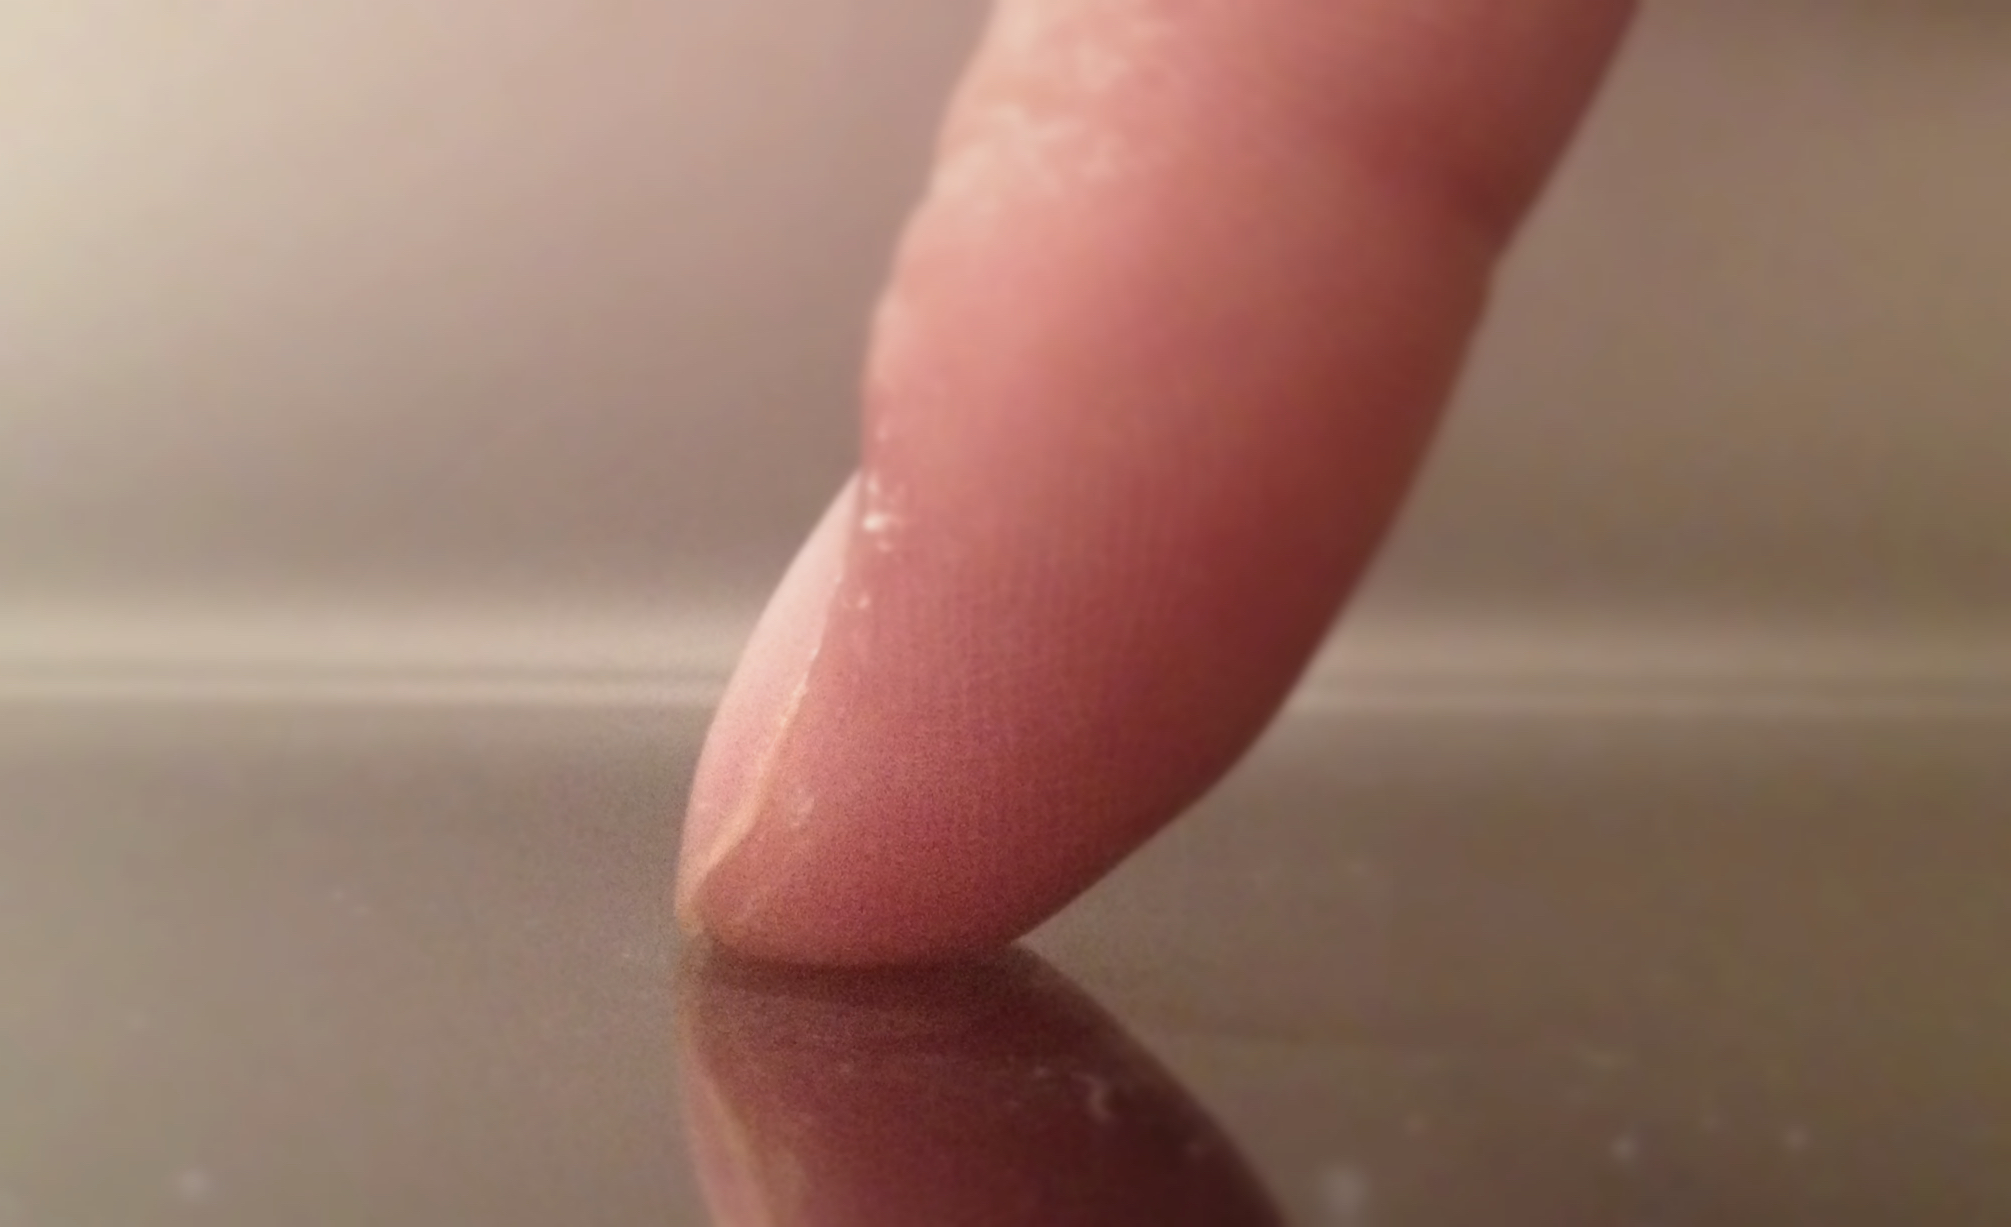
\includegraphics[width=\textwidth]{figures/ffmin}
	\caption{Minimum contact size position}
	\label{fig:ffmin}
\end{subfigure}
\hfill
\begin{subfigure}[b]{0.4\textwidth}
	\centering
	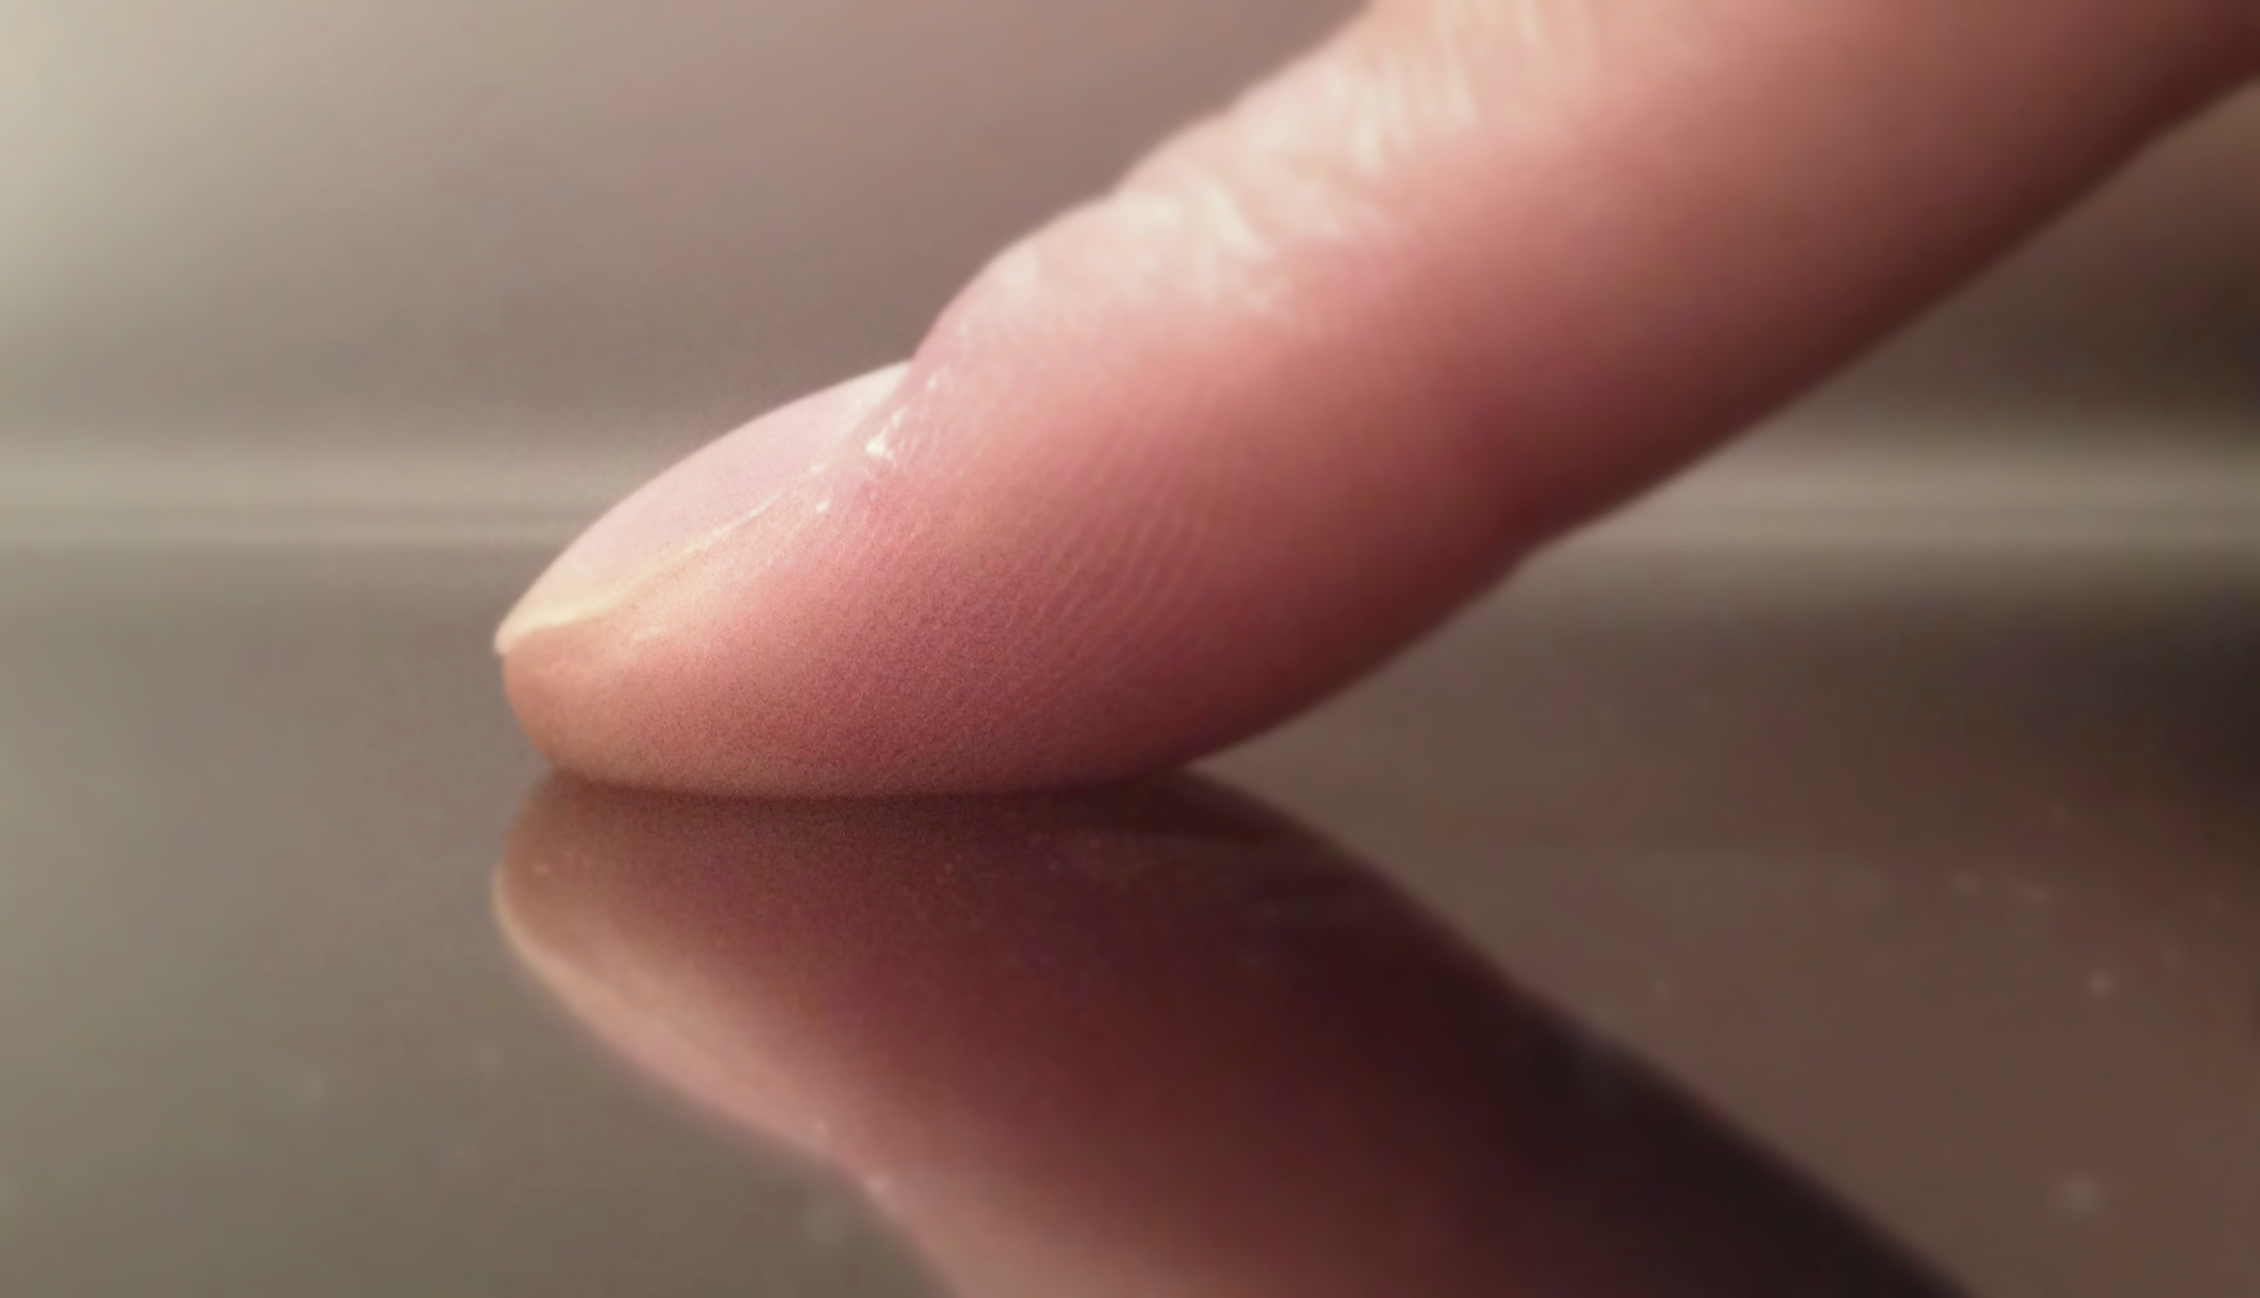
\includegraphics[width=\textwidth]{figures/ffmax}
	\caption{Maximum contact size position}
	\label{fig:ffmax}
\end{subfigure}
\caption{Demonstration of a minimum and a maximum contact size hand position}
\label{fig:ffMinMax}
\end{figure}

%%%%%%%%%%%%%%%%%%%%%%%%%%%%%
%%%%%%%%%%%%%%%%%%%%%%%%%%%%%
%%%%%%%%%%%%%%%%%%%%%%%%%%%%%
%%%%%%%%%%%%%%%%%%%%%%%%%%%%%
%%%%%%%%%%%%%%%%%%%%%%%%%%%%%
%%%%%%%%%%%%%%%%%%%%%%%%%%%%%
\subsection{Assessment}
\label{assessment}


After having completed all the trials, participants instructed to fill a questionnaire to access, rate and finally comment on each of the type of trials they encountered. The questionnaire (Appendix \ref{assessmentFatFinger}) was divided if 4 parts, one for each targeting technique. So, participants had to provide an assessment for all the following type of trials:

 1)\textbf{Feedback \& Discrete Targeting} 2) \textbf{Feedback \& Continuous Targeting} 3) \textbf{No Feedback \& Discrete Targeting} 4) \textbf{No Feedback \& Continuous Targeting}


The assessments had the same structure, and were independent of the type of the trials. Each assessment consists of 6 categories, all on a five point Likert scale. The categories were:


\begin{itemize}
\item \textbf{Smoothness during operation.} The user should rate the smoothness during the operation of the specified Trial type. Smoothness behaves as a general factor that is totally subjective. Signs of roughness can be a slow rate frame in the graphics, or lack on the accuracy of the feedback line. 

\emph{\textbf{Scale}: Very rough (1) - Very smooth (5)}.


\item \textbf{Operation speed.} It can be anything at all. If participants had the feeling the everything flows in a normal rate then the should rate it with 3 which is the normal speed. In this index the best rating is considered 3.

\emph{\textbf{Scale}: Too fast (1) - 2 - Normal (3) - 4 - Too slow (5)}.

\item \textbf{Finger fatigue.} Participants here can record the level of finger fatigue through the corresponding type of trial in this experiment.

\emph{\textbf{Scale}: None (1) - Very high (5)}.

\item \textbf{Wrist fatigue.} Participants here can record the level of wrist fatigue through the corresponding type of trial in experiment.

\emph{\textbf{Scale}: None (1) - Very high (5)}.

\item \textbf{General comfort.} The meaning is inferred from its name. What we ask for, is a general impression on how comfortable this type of trial was. Of course there is interference between this factor and the wrist and finger fatigue ones. However, a type of trial might be comfortable under normal use, but it may cose fatigue in longer use.

\emph{\textbf{Scale}: Very uncomfortable (1) - Very comfortable (5)}.

\item \textbf{Overall assessment.} It measures the general impression of this type. It is measured in usability factors. Thus rating 1 means that it was easy to use and in turn, rating 5 that it was really tough to use it.

\emph{\textbf{Scale}: Very difficult to use (1) - Very easy to use (5)}.
\end{itemize}

Finally, at the bottom of each page there was a comment section, in which participants was asked to comment any advantages or disadvantages they might have encountered during the operation of each type of trial. It was not a required section, however many participants shared their thoughts with us, and we did extracted some really important results out of them.









%%%%%%%%%%%%%%%%%%%%%%%%%%%%%
%%%%%%%%%%%%%%%%%%%%%%%%%%%%%
%%%%%%%%%%%%%%%%%%%%%%%%%%%%%
%%%%%%%%%%%%%%%%%%%%%%%%%%%%%
%%%%%%%%%%%%%%%%%%%%%%%%%%%%%
%%%%%%%%%%%%%%%%%%%%%%%%%%%%%
\section{Participants}

We recruited 26 participants to participate in our study ranging in age from 19 to 52 years old. They had to fill in a Demographic information form from which we collected the following info.

\begin{figure}[H]
\centering
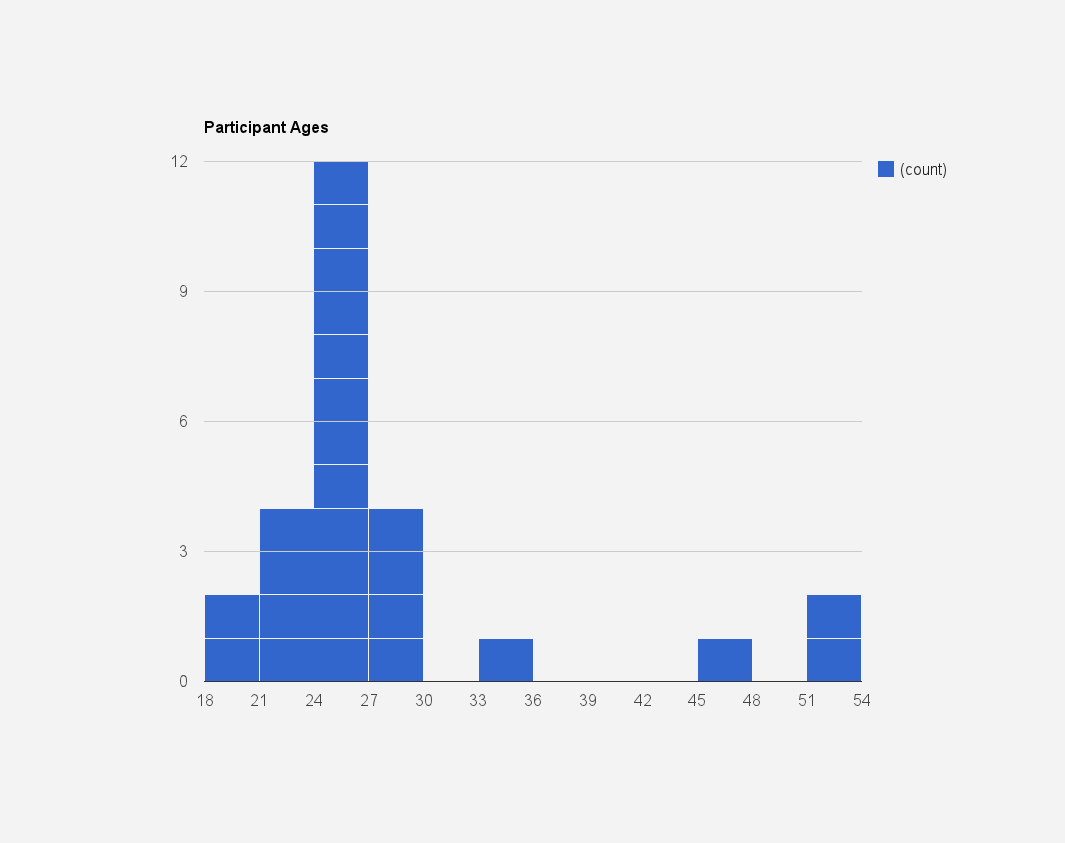
\includegraphics[scale=0.3]{figures/participantAge.png}
\caption{Distribution of participant ages}
\label{fig:participantAge}
\end{figure}

As we can see from Figure \ref{fig:participantAge} participants are mostly ranged between 21 and 30 years old. We also tried to recruit people from older ages, which they might had a different level of experience with tablet devices. therefore we have 2 participants on the 33-48 range and other 2 that are above 50 years old.

\begin{figure}[H]
\centering
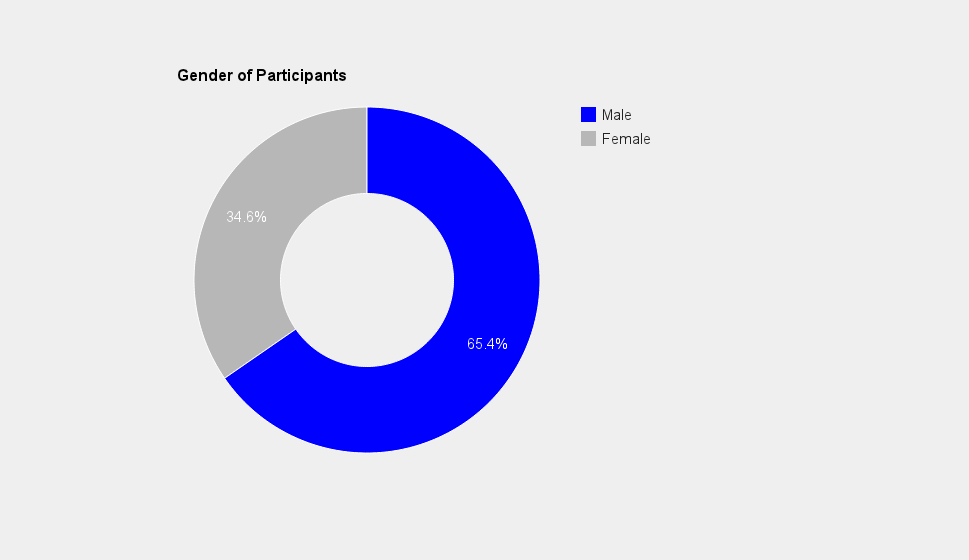
\includegraphics[scale=0.3]{figures/participantGender.png}
\caption{Distribution of participants Gender}
\label{fig:participantGender}
\end{figure}

Participants were mostly male (65.4\%) as it can be observed on Figure \ref{fig:participantGender}. To be precise, we had 17 participants that were male and also 9 more that were female (34.6\%). Also 24 of them were right-handed while only 2 used their left hand for the experiment. Moreover only 21 of them owns a touch based device of any possible kind, and from those just 12 own an actual Tablet device. A mobile, a GPS etc. can be regarded as touch based Devices. We can then conclude that less than half of the users owns a Tablet device, and not specifically an Apple iPad one.

In Figures \ref{fig:experienceTouch}, \ref{fig:experienceTablet} is illustrated how users rated their level of experience on using Touch-Based and Tablet devices respectively.

\begin{figure}[H]
\centering
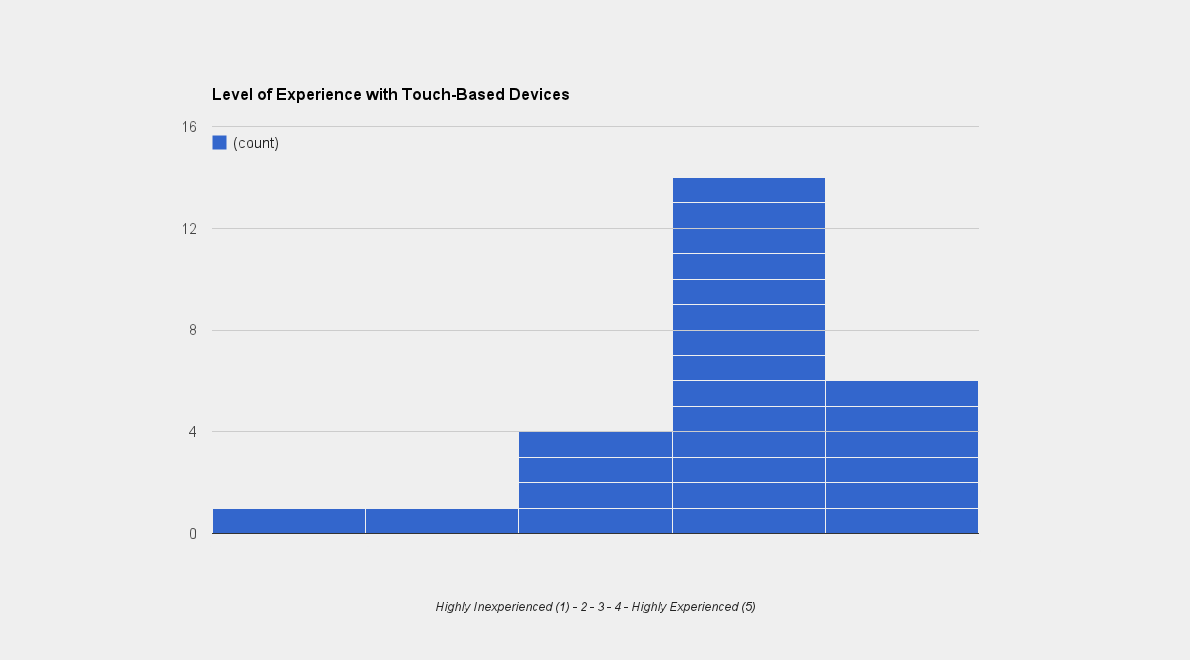
\includegraphics[scale=0.3]{figures/experienceTouch.png}
\caption{Level of Experience with Touch-Based Devices}
\label{fig:experienceTouch}
\end{figure}

\begin{figure}[H]
\centering
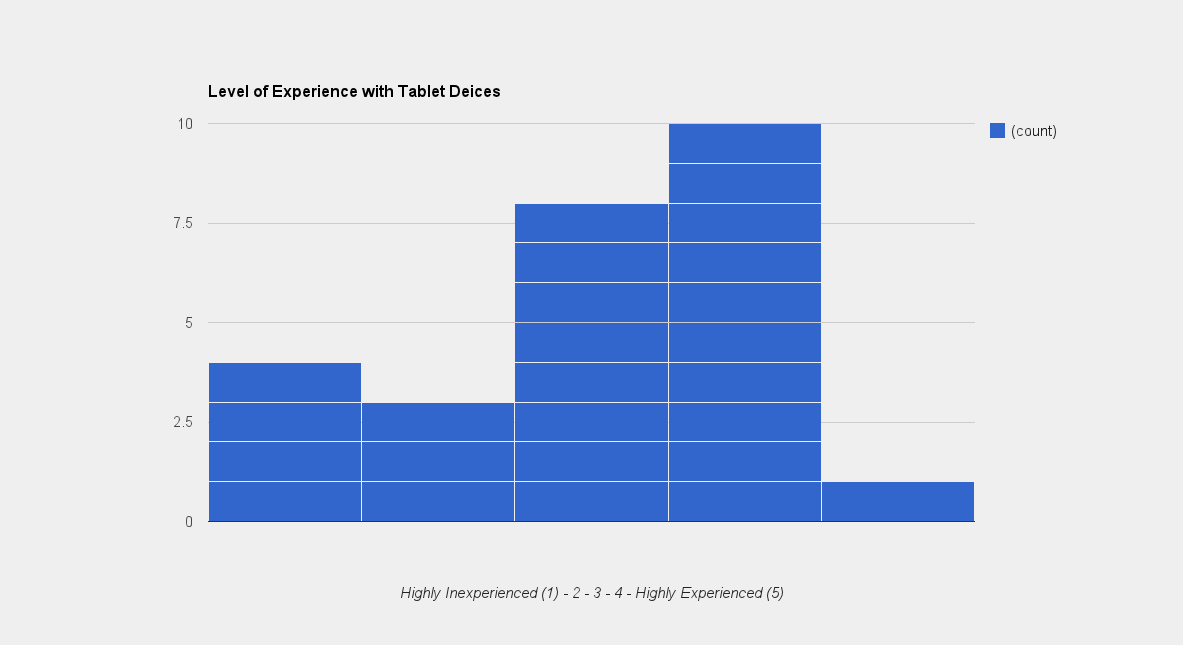
\includegraphics[scale=0.3]{figures/experienceTablet.png}
\caption{Level of Experience with Tablet Devices}
\label{fig:experienceTablet}
\end{figure}

In the above charts, each buckets represents a participant. The more on the right the buckets is (only 5 levels), the more experience this participant has, and vise versa. Thus, we can observe that most of them were experienced using touch-based mobile devices, while fewer were high experienced addressing the tablet devices. This can also be inferred from to the fact that less than half the users owes a tablet device. As a result they have less experience on using one. Finally, it should be mentioned that participants received a small gift, as compensation for their time and effort.




\section{Hypotheses}
\label{sec:hypotheses}

According to and based on our understudying of Fat Finger and on using contact size as the main source for input on tablet devices, we hypothesize the following:

\begin{itemize}
	\item \textbf{\textit{(H1).}} Feedback supplied trials (Discrete or Continuous) outperform No Feedback ones in terms of offset.
	\item \textbf{\textit{(H2).}} No Feedback \& Discrete outperforms No Feedback \& Continuous in terms of offset.
	\item \textbf{\textit{(H3).}} Task completion time will be gradually decreased over time.
	\item \textbf{\textit{(H4).}} Error rates will be gradually decreased over time.
	\item \textbf{\textit{(H5).}} Task competition time, when feedback is provided, is dependent on the number of elements.
	\item \textbf{\textit{(H6).}} Average contact areas will be subconsciously preferred by users, as this is the natural position of the finger.
	\item \textbf{\textit{(H7).}} Feedback \& Discrete is the most preferred type of trial, as it best combines speed and accuracy.
\end{itemize}





\cleardoublepage


\chapter{Results}
\label{sec:Results}
This chapter presents all the results we collected after performing the user study on Fat Finger interaction technique. We decided to focus on 5 basic results categories - parameters, which include the most significant information we collected and analysed. We present the results for Task Completion Time, Offsets, Learning Curve, Re-Entries - Re-Touches and Subjective Preferences. We also refer to the categories of the trials with the shortages presented in Table \ref{tab:typeIDnames}. This will help the reader to better understand and interpret the various graphs presented later.

\begin{table}[H]
\centering
\begin{tabular}{l || c || c }
Name & Code-Name & TypeID \\
\hline
\hline
Feedback \& Discrete & FD & 1 \\
Feedback \& Continuous & FC & 2 \\
No Feedback \& Discrete & NFD & 3 \\
No Feedback \& Continuous & NFC & 4 \\
\end{tabular}
\caption{Code names for the 4 categories of trials}
\label{tab:typeIDnames}
\end{table}


%%%%%%%%%%%%%%%%%%%%%%%%%%%%%
%%%%%%%%%%%%%%%%%%%%%%%%%%%%%
%%%%%%%%%%%%%%%%%%%%%%%%%%%%%
%%%%%%%%%%%%%%%%%%%%%%%%%%%%%
%%%%%%%%%%%%%%%%%%%%%%%%%%%%%
%%%%%%%%%%%%%%%%%%%%%%%%%%%%%
\section{Task Completion Time}
\label{sec:resultsTaskCompletionTime}

Task completion time is a parameter that counts the total time the participant spent on a specific trial. As mentioned in section \ref{sec:monitoring}, the timer fires when the first touch is performed and stops counting when the confirming sound is being played, which indicates that we successfully hit the target. Also in Feedback trials we use the Dwell selection technique. that adds an 1s delay. In No-Feedback trials there is no such time constraint, since we use the Quickrelease method (no obligatory delay) to perform target selection. 

We performed a $4 * 7$ (TypeID $*$ N) within subjects ANalysis Of VAriance (ANOVA) \cite{anova}, using the aggregated values of total time. We use ANOVA to determine if the mean values for offset are statistically different. Of course, we can export basic information about the means by just comparing them, but we want to know what do these directional differences in the means infer about our results. ANOVA is able to determine if the differences between condition means are significant.

\begin{figure}[H]
\centering
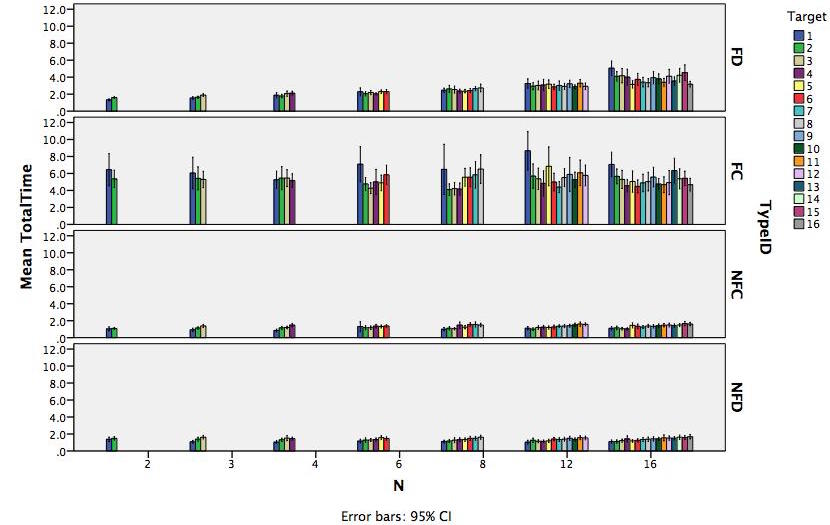
\includegraphics[width=\textwidth]{figures/meanTotalTime}
\caption{Total Time panelled by TypeID  - 95\% Confidence Interval}
\label{fig:meanTotalTime}
\end{figure}

Figure \ref{fig:meanTotalTime} illustrates the aggregated task completion time values, panel-by typeID and cluster-by the number of buckets (N).
 We found that Mauchly's Test of Sphericity is violated for all Type of Trial (TypeID), number of elements (N), and also their combination (TypeID*N). That means that the type of the trial, the number of elements and their combination have a significant effect on completion time. We found that Grand Mean is \emph{2.619} seconds (STD = \emph{0.142s}). Feedback \& Discrete (M = \emph{2.387s} STD = \emph{0.084s}) was really fast, taking into consideration that it expects \emph{1s} delay to confirm target selection.
  No Feedback \& Discrete (M = \emph{1.237s} and STD = \emph{0.093s}) and No Feedback \& Continuous (M = \emph{1.365s} and STD = \emph{0.013s}) were ranked almost equally and were the fastest. Feedback \& Continuous (\emph{M = 5.485} and \emph{STD = 0.457}) was the slowest one, but this can be partly explained from the fact that on the one hand, it contained the smallest targets, and on the other, the user had to pass the \emph{1s} inside target delay. Stay for \emph{1s} inside a designated small area can be really difficult under certain conditions.

Table \ref{tab:totaTimeAnova} presents the mean differences between all possible combination of the type of Trials (TypeID). As we can see, and  as already stated, Mean differences are really significant for all possible combinations.

\begin{table}[H]
\centering
\begin{tabular}{c || c || c || c}
TypeID (i) & TypeID (j) & Mean Difference (i-j) & Sig. \\
\hline \hline
FD      &   FC      &   -3.098      & 0.000 \\
FD      &   NFD     &   1.151       & 0.000 \\
FD      &   NFC     &   1.022       & 0.000 \\
FC      &   NFD     &   4.249       & 0.000 \\
FC      &   NFC     &   4.120       & 0.000 \\
NFD     &   NFC     &   -0.129      & 0.002
\end{tabular}
\caption{Task Completion Time: Mean differences among the different types of Trials}
\label{tab:totaTimeAnova}
\end{table}

Type of Elements (N), is a parameter that specifies the size of the target for Discrete trials and also the position of it, depending on which is the target bucket out of the N specified. In Continuous trials the size of each trial is independent of the number of elements (N), and is stable, however, N limits the position of the target under a specific region. 
Lower values for N result in a wider space range (\emph{N=2} and \emph{TargetBucket=1} means that the target can be anywhere inside the lower semicircle), while higher values significantly narrow this range (\emph{N=16} and \emph{TargetBucket=1} means that the target will be somewhere really close to the minimum value).

We found that task completion time does not statistically differ for \emph{N = 2, 3, 4, 6, 8}. For all those different type of elements the Mean differences are not statistically different, thus we can conclude that they behave quite similarly. However, as expected, the scenario is different for 12 and 16 Elements. For \emph{N=12} we detect significant differences with \emph{N=2} (Sig. = 0.024) and \emph{N=3} (Sig. = 0.017), while for the rest we have no significant differences (Sig. values $>$ 0.05). However \emph{N=16} differs significantly with all the aforementioned \emph{N}'s, apart from \emph{N=12}. 

The combination of the number of Elements (N) and the type of Trials, in turn points out some other important results too. For FC, NFD and NFC we observe that the number of Elements does not influence that task completion time. We have very similar completion times which are independent of N. Specifically, for \emph{Feedback \& Continuous} time for all possible N's is around 5.485 seconds, for \emph{No Feedback \& Discrete} around 1.237 seconds and for \emph{No Feedback \& Continuous} around 1.365.
 However, interest is really triggered when we check the values for \emph{Feedback \& Discrete} targeting. The completion time  is significantly increased as the number of Elements increases. We start with \emph{1.460 s} for \emph{N=2} and we end up with \emph{3.858 s} for \emph{N=16}. Completion time accordingly gradually increases for all intermediate N values, which supports H5. For \emph{N=16} we have that bucket size is still bigger that the size of a continuous target (offset range including). We expect that for even smaller targets, as in \emph{Feedback \& Continuous}, the completion time will be even higher, as the target range is smaller. This claim indeed holds. We saw above that for FC the completion time is stable and independent on the number of elements (\emph{N}), which makes sense because in FC target size does not even change. Summarizing we can conclude that:
\emph{
\begin{itemize}
    \item When feedback is provided, completion time is highly dependent on the size of the target, increasing as the target size decreases. 
    \item When feedback is provided, completion time is statistically independent for N values up to 8 buckets.
    \item In No Feedback trials, completion time is independent of the size of the buckets.
\end{itemize}
}











%%%%%%%%%%%%%%%%%%%%%%%%%%%%%
%%%%%%%%%%%%%%%%%%%%%%%%%%%%%
%%%%%%%%%%%%%%%%%%%%%%%%%%%%%
%%%%%%%%%%%%%%%%%%%%%%%%%%%%%
%%%%%%%%%%%%%%%%%%%%%%%%%%%%%
%%%%%%%%%%%%%%%%%%%%%%%%%%%%%
\section{Offsets}
\label{sec:resultsOffset}

Offset is a parameter that generally represents the error for each trial. Error is measured by the percentage we were off the target. For instance, imagine that we have a target of type Continuous, placed on $x$ degrees, but we confirm selection at $y$ degrees, with $x\neq y$. Then the error is the difference of x and y, $x-y$. In other words it is the distance from the point we selected to the center of the target, compared to the whole range (\emph{360 degrees}). 
This difference produces a positive number if the confirmed contact size is bigger that the target's ($y>x$), and negative otherwise ($y<x$). Thus error rates can either be negative or positive depending on whether we performed selection before or after the target respectively. 
We also decided not to measure offset for FD trials, as there is no way that users can perform errors in those trials. Users were instructed to hit the target at whichever point inside its range, and not implicitly at the center of it. 
However, in No-Feedback trials the participant can confirm selection even if he is outside the target. Thus, error measurement is a much significant parameter, we need to analyse and export for those trials.

We aggregated the Offset values for each user, and with the aggregated offsets we performed a $3 * 7$ (\emph{TypeID $*$ N}) within subjects ANalysis Of VAriance. We found that Grand Offset Mean is \emph{11\%} , which can be translated into $39.6$ degrees ( \emph{11\% * 360 degrees}).
It is vital to mention that grand mean is much influenced from No Feedback trial values since, Feedback \& Continuous does not allow high values for error; simply because you can not select a target if you are outside the yellow lines. 
The range of the yellow lines is \emph{4\%}, thus errors are limited in the \emph{+-2\%} region. 
For Feedback \& Continuous trials, Mean offset is \emph{1,1\%} and STandard Deviation (STD) \emph{0,1\%}.
On the other hand, offset values are significantly increased in No Feedback trials. Well interestingly, both Feedback \& Discrete and No-Feedback \& Continuous share the same Mean offset values: \emph{Mean offset = 16,1\% and STD=1,1\%}.


Applying ANOVA and Post Hoc multiple means comparisons we found that \textbf{none} of the number of buckets (\emph{N}), the type of the Trials and the combination of them have an effect on the error rate - offset. Moreover we discovered that (including all possible N values) there is no significant difference between NFD and NFC (\emph{Sig = 1}).
We can conclude that the differences between those offset Means are likely due to chance and probably not due to the type of the trials.
Actually it is very interesting that NFD and NFC behave exactly the same along the experiment, which might infer that success rate of no feedback supported trials is not dependent on the size of the target.
Also, as expected FC behave differently ($Sig=0.000 \leq 0.05$) with both NFD and NFC.

Figure \ref{fig:meanOffset} illustrates the aggregated Offset values, panel-by typeID and cluster-by the number of buckets (\emph{N}). Observing the graph we can extract some meaningful results:

\begin{enumerate}
    \item \textbf{In FC error rates are always very small apart from a sudden increase they have for the last bucket of each N}. We attribute that to the fact that when the target was close to the maximum point (\emph{360 degrees}) users used to apply full pressure, ans so reach the maximum level, than trying to achieve high precision on the target by hitting it accurately. 

    \item \textbf{In NFD and NFC error rates follow a common pattern}. For the first buckets of each N they are positive, and they start going gradually negative as we move to the last buckets. This can be partly explained from the fact that average contact sizes are much easier to get achieved. When our finger simply touches the screen with, it is more likely to be somewhere between the minimum and the maximum area, that close to the limits. This is the natural position of our finger when are simply touching the screen.

    We realize then, that participants tend to go closer to this normalized area. They seem to have better control there, and more comfort too. This is probably why we observe that pattern on the graphs. When target are really close to the limits we tend to select areas that are closer to the normalized region than the correct ones.
\end{enumerate}
%%
%% FIG: Offset aggregated 
%%
\begin{figure}[H]
\centering
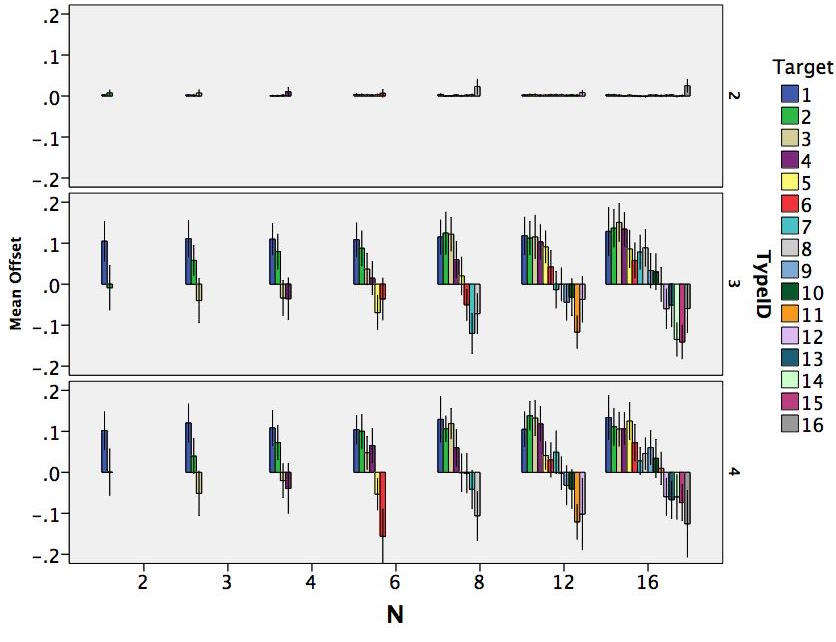
\includegraphics[width=\textwidth]{figures/meanOffset}
\caption{Offset aggregated - 95\% Confidence Interval}
\label{fig:meanOffset}
\end{figure}


After observing the error rates, it would be also nice to  take a look on the No Feedback trials success rate. Table \ref{tab:ffHitInside} presents the percentage of successful selections for both No Feedback \& Discrete and No Feedback \& Continuous. For Discrete targets the successful trials (\emph{33\%}) are much more than for the Continuous targets (\emph{11\%}).However they share the same error rates as mentioned above. How is that even possible?

Well, for Discrete targets we count the offset from the middle of each target. For instance,  if $N=2$ then the middle of the first bucket (down semicircle) is at \emph{90 degrees}. Even if the offset is \emph{25\%} ($=90 degrees$) then we are still inside the target, at the edge of it though. The same applies for higher \emph{N} values, but the 'permited'  offset is then narrower. Summarizing:

\emph{Offset values for Discrete targeting are not always considered as errors, as we measure offset from the center of the targets range. The real error can be calculated by the type:}   $RealErrorDisrete = OffsetValue - (TargetRange*0.5)$



\begin{table}[H]
\centering
\begin{tabular}{l || c | c }
 & Successful & Unsuccessful \\
\hline
\hline
NFD & 33.76\% & 66.16\% \\
NFC & 11.25\% & 88.75\% 
\end{tabular}
\caption{No Feedback: Percentage of successful hits}
\label{tab:ffHitInside}
\end{table}


% %%
% %% FIG: Hit Inside
% %%
% \begin{figure}[H]
% \centering
% \begin{subfigure}[b]{0.4\textwidth}
%     \centering
%     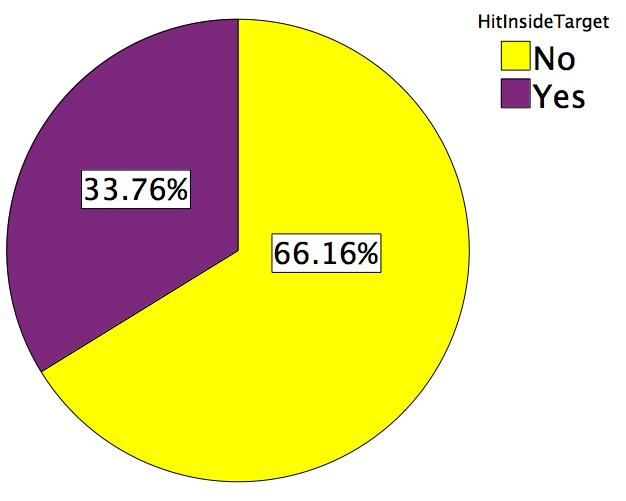
\includegraphics[width=\textwidth]{figures/hitInsideNFD}
%     \caption{Success ratio for No Feedback \& Discrete}
%     \label{fig:ffHitInsideNFD}
% \end{subfigure}
% \hfill
% \begin{subfigure}[b]{0.4\textwidth}
%     \centering
%     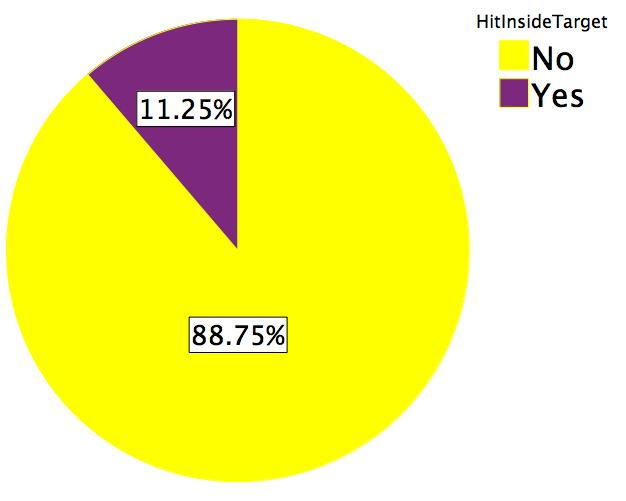
\includegraphics[width=\textwidth]{figures/hitInsideNFND}
%     \caption{Success ratio for No Feedback \& Continuous}
%     \label{fig:ffHitInsideNFND}
% \end{subfigure}
% \caption{Percentage of successfully hit No Feedback trials}
% \label{fig:ffHitInside}
% \end{figure}




%%%%%%%%%%%%%%%%%%%%%%%%%%%%%
%%%%%%%%%%%%%%%%%%%%%%%%%%%%%
%%%%%%%%%%%%%%%%%%%%%%%%%%%%%
%%%%%%%%%%%%%%%%%%%%%%%%%%%%%
%%%%%%%%%%%%%%%%%%%%%%%%%%%%%
%%%%%%%%%%%%%%%%%%%%%%%%%%%%%
\section{Learning Curve}
\label{resultsLearningCurve}

In section \ref{sec:FinalSequenceofTrials} we mentioned that training phase is not isolated from the rest of the experiment. Our approach is to use to use a 3-repetition design (Figure \ref{fig:ffRepetitions}), in which the first repetition will also act as the Learning phase, while the remaining 2 would just be the normal experiment. 
This way we are not eliminating learning from performing phase and most importantly, this give us the possibility to monitor the way and the pace the participants are getting used to this new interaction technique and observe the improvements of performance over time. In other words, this design provide us the appropriate tools for building the Learning Curve of Fat Finger.

    %%%%%%%%
    %%%%%%%%
    %%%%%%%%
\subsection{Total Time}
\label{sec:LCtotalTime}
We hypothesized (H3) that the average total time needed for the completion of each trial will be decreased over time. In other words we hypothesized that:

 $AverageTimeRepetition1 > AverageTimeRepetition2 > AverageTimeRepetition3$ 

Figure \ref{fig:learningCurveTotal} presents the average completion time learning curve in each repetition. We can observe that for repetition \emph{No 1} the mean time is just above \emph{3 seconds}. In Repetitions \emph{No 2} and \emph{No 3} the time decreased down to around \emph{2.5 seconds}. Thus we have a learning factor over time, especially between repetition \emph{No 1} and repetition \emph{No 2}. Repetition \emph{3} whilst not obviously improving the average trial time, is still contributing in the Learning effect in regards of specific trials; as I will thoroughly explain onwards. 
%%%%
%%%%
%% Total time Learinng Curve
%%%%
%%%%

\begin{figure}[H]
\centering
\begin{subfigure}[b]{0.45\textwidth}
    \centering
    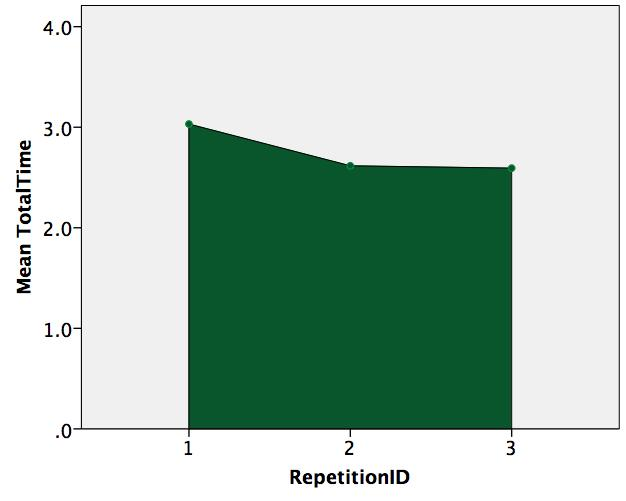
\includegraphics[width=\textwidth]{figures/learningCurveTotal}
    \caption{Learning Curve - Overall Total Time }
    \label{fig:learningCurveTotal}
\end{subfigure}
\hfill
\begin{subfigure}[b]{0.45\textwidth}
    \centering
    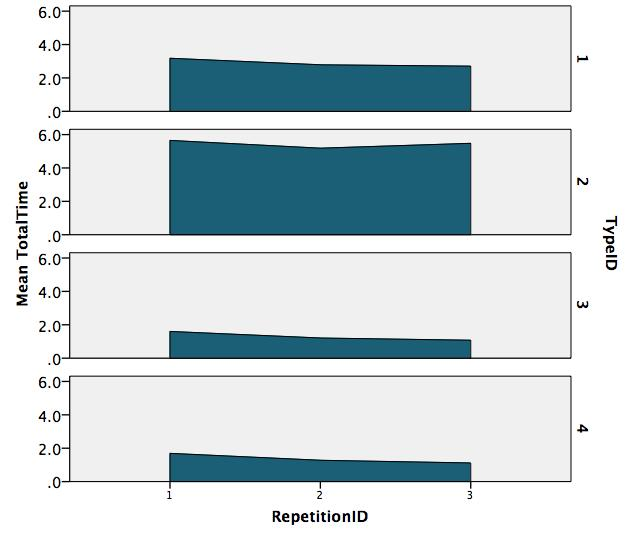
\includegraphics[width=\textwidth]{figures/learningCurve}
    \caption{Learning Curve - Time by TypeID}
    \label{fig:learningCurve}
\end{subfigure}
\caption{ Learning Curve - Task Completion Time}
\label{fig:learningCurveTotalTime}
\end{figure}



Figure \ref{fig:learningCurve} presents the average completion time learning curve in each repetition, panelled by Trial category (\emph{typeID}).
Learning curve for NFD ($TypeID = 3$) and NFC ($TypeID = 4$) depicts a continuous improvement of the average completion time among repetitions. However, the error rates learning curve as we point out in section \ref{sec:LCOffset}, have a completely reversed behaviour over time. 
Feedback \& Discrete learning curve follows the same behaviour as the overall time learning curve in \ref{fig:learningCurveTotal}.
On the other hand, Feedback \& continuous is the only type of trials for which, we do not observe continuous improvement over time. However, whilst being slower his error rates constantly decrease over time (section \ref{sec:LCOffset}). Thus, higher time values does not necessarily mean that our performance is being degraded.
 % Learning factor is a multi factor parameter, which mainly consists of the time and the error rate parameters. 

Taking into account the aforementioned graphs, we realize that there exist obvious learning improvements over time. However while for repetition \emph{No 1} to repetition \emph{No 2} we do observe significant learning factors, this is not that obvious for repetition \emph{No 3}. Mental and physical fatigue might have a share in this behaviour. While we do not have any measurement for fatigue to validate this claim, we can however extract some meaningful results from the assessments participants provided us at the end of each experiment. A short conclusion would be: if it was not for fatigue (mental and physical), learning curve might have been further decreased on repetition 3. 

%Finally, we encountered very few users that were really crummy during repetition 3, resulting in exponential increase in their total time. Ruling out these cases, we indeed have that average total time was further decreased on repetition 3. 

    %%%%%%%%
    %%%%%%%%
    %%%%%%%%
\subsection{Offset}
\label{sec:LCOffset}
In Figure \ref{fig:learningCurveOffset} we can observe the behaviour of Error rates along the repetitions, and use that knowledge to extract results regarding the error rates learning curve for all Feedback \& Continuous (blue), No Feedback \& Discrete (green) and No Feedback \& Continuous (red) trials. 

As we can notice, there is no significant improvement of the error rates over time, neither for FC (1,1\% - 1,1\% - 1\%), nor for NFC (16,3\% - 15,9\% - 16\%). The differences are on the 0,1\% scale which is not even noticeable. However in No Feedback \& Discrete trials (green) we do observe a drop of 2\% on the second repetition, but a slight increase (0,5\%) on the third one.
According to the aforementioned values, we realize that error rates are not subject to the same learning factor we experienced for Task Completion time in section \ref{sec:LCtotalTime}. However, the fact that we did not meet increasing values along the repetitions, is very promising. It infers that users are capable to maintain the same error rates, which are relatively low, along by decreasing their competition time.




%%%%
%%%%
%% OFFSET Learning Curve
%%%%
%%%%
% \begin{figure}[H]
% \centering
% \begin{subfigure}[b]{0.45\textwidth}
%     \centering
%     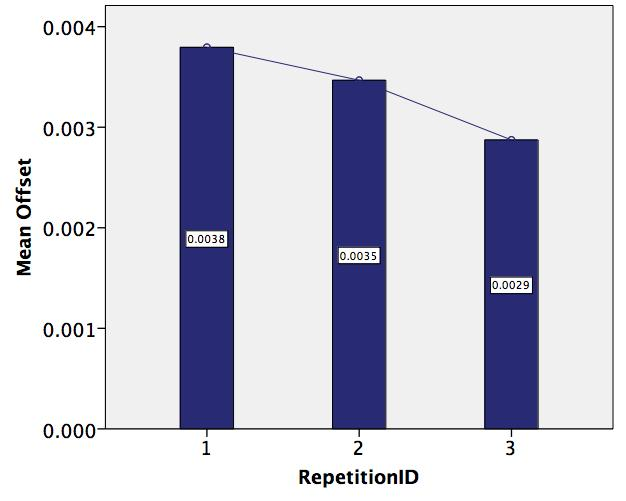
\includegraphics[width=\textwidth]{figures/learningCurveOffsetFC}
%     \caption{Error Rate Learning Curve - Feedback \& Continuous}
%     \label{fig:learningCurveOffsetFC}
% \end{subfigure}
% \hfill
% \begin{subfigure}[b]{0.45\textwidth}
%     \centering
%     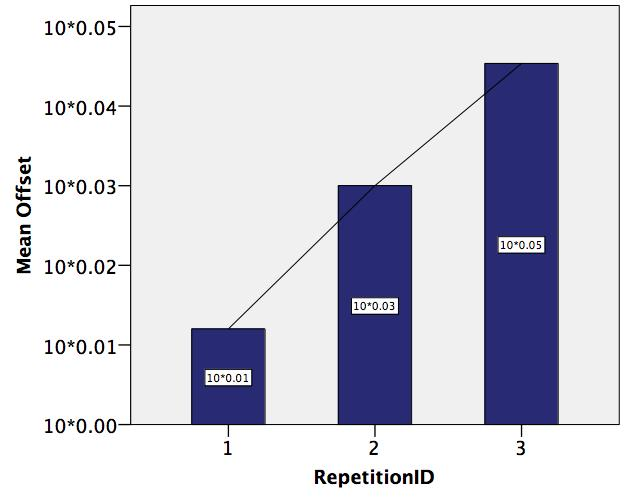
\includegraphics[width=\textwidth]{figures/learningCurveOffsetNF}
%     \caption{Error Rate Learning Curve - No Feedback Trials}
%     \label{fig:learningCurveOffsetNF}
% \end{subfigure}
% \caption{Error Rate Learning Curve}
% \label{fig:learningCurveOffset}
% \end{figure}


\begin{figure}[H]
\centering
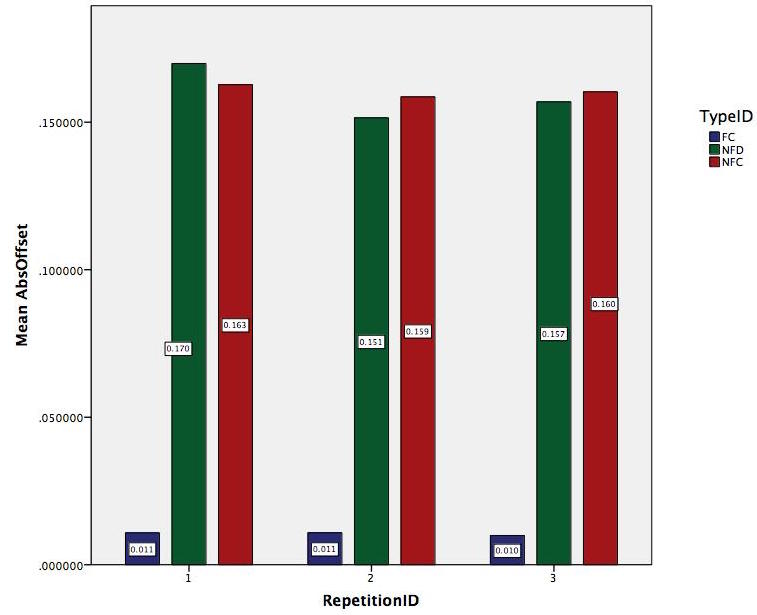
\includegraphics[width=\textwidth]{figures/learningCurveOffset}
\caption{Learning Curve - Offset}
\label{fig:learningCurveOffset}
\end{figure}


One important thing to note is, that certain values for error are affordable in No Feedback trials. Especially for No Feedback \& Discrete Targeting that maximum affordable error is presented on Table \ref{tab:NFDAffordableError}. It can be calculated using the type:

 $AffrodableError = (\frac{100}{N} = BucketSize) * \frac{1}{2}$

Affordable error is half of the size of its bucket for a specific N. Now, by combining the data from Table \ref{tab:NFDAffordableError} and Figure \ref{fig:learningCurveOffset} we can extract even more meaningful and interesting results. With the given error rates for NFD, we find that for $N=2$ or $N=3$, we will always perform selection inside the target area. That happens because the average error rates are lower than the affordable error, meaning that this error is indeed acceptable and thus we successfully performed an in-target selection. We also realize than hitting smaller targets ($N>4$), is not trivial in No Feedback trials since average error rates are much higher compared to the maximum affordable error rates for those N values.

% However, no matter of which the affordable error might have been, we still experienced quite high error rates, which were increased in each repetition. This can be partly interpreted if we take into account that No Feedback trials were really difficult for the users and required utter focusing from their side. Concentrating on the trial, was getting more and more difficult over time, due to the mental and physical fatigue. Thus users tent to have better scores on the first repetition than in the following two. In particular average error was \emph{12\%} for repetition \emph{1}, \emph{30\%} on the \emph{2nd} repetition and \emph{45\%} on the last one. This sudden and steep increase of the error values, supports our argument that users after a certain amount of time experienced fatigue and partly lost their focus on these type of trials.


\begin{table}[H]
\centering
\begin{tabular}{l || c}
N & Maximum affordable error in \% \\
\hline \hline
\textbf{2} & 25,00\% \\
\textbf{3} & 16,66\% \\
\textbf{4} & 12,50\% \\
\textbf{6} & 08,33\% \\
\textbf{8} & 06,25\% \\
\textbf{12} & 04,16\% \\
\textbf{16} & 03,12\% 
\end{tabular}
\caption{Fat Finger - No Feedback \& Discrete Targeting affordable error}
\label{tab:NFDAffordableError}
\end{table}






%%%%%%%%%%%%%%%%%%%%%%%%%%%%%
%%%%%%%%%%%%%%%%%%%%%%%%%%%%%
%%%%%%%%%%%%%%%%%%%%%%%%%%%%%
%%%%%%%%%%%%%%%%%%%%%%%%%%%%%
%%%%%%%%%%%%%%%%%%%%%%%%%%%%%
%%%%%%%%%%%%%%%%%%%%%%%%%%%%%
\section{Re-Entries}
\label{resultsReEntries}

Analysis of the target Re-Entries that occurred during the whole experiment will help us to better understand where users faced difficulties, caused by tremolo or general stabilization parameters. We meet higher values for target re-entries, when the target's range is smaller. As we will see onwards, when the finger of participant was not completely accurate and stable, the tremolo produced was enough, to cause small and usually fast movement of the feedback region. If the feedback edge was close enough to the edge of the target, then this slight movement ("in" and "out" of the target region) was encountered as 1 re-entry. 

Figure \ref{fig:meanReentries} presents the average target re-entries for each of the trial categories and  all possible \textbf{N}'s. \textbf{Feedback \& Discrete} has almost zero re-entries per trial especially for low values of N. When N increases re-entries follow along and we reach a maximum of around \emph{1.5} target re-entries per trial (\emph{N=16}). This enhances and further supports the claim we made before about the connection between target size and target re-entries.
\textbf{Feedback \& Continuous} have almost the same number of target re-entries as the size of the target is independent of the value of \emph{N}. The range of the target is even smaller that the FD one of \emph{N=16}, so the target re-entries per trial are even higher than the maximum value for Feedback \& Discrete targeting. We have an average of around 2 target re-entries for all Feedback \& Continuous trials. 
\textbf{No Feedback \& Discrete} and \textbf{No Feedback \& Continuous} have almost the same reaction regarding target re-entries. Since users are not aware of the position of the feedback region, and they need to stay inside the target for a specific time; they just move their finger in the desired position and then simply lift it. Thus, movements such as trembling around a specific area for a long time to stay accurate did not encountered. As a result target re-entries are too low; \emph{0.5} per trial or differently expressed, one every two trials. So for NF trials, target re-entries are independent both from the target's size and from the of trial (NFD or NFC). 


\begin{figure}[H]
\centering
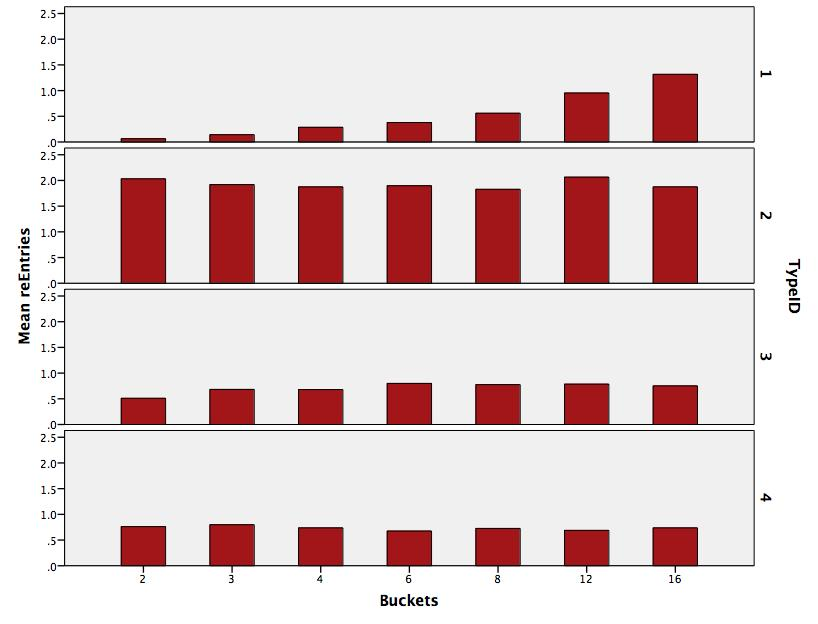
\includegraphics[scale=0.4]{figures/meanReentries}
\caption{Target Re-Entries panelled by Type of Trial}
\label{fig:meanReentries}
\end{figure}


%%%%%%%%%%%%%%%%%%%%%%%%%%%%%
%%%%%%%%%%%%%%%%%%%%%%%%%%%%%
%%%%%%%%%%%%%%%%%%%%%%%%%%%%%
%%%%%%%%%%%%%%%%%%%%%%%%%%%%%
%%%%%%%%%%%%%%%%%%%%%%%%%%%%%
%%%%%%%%%%%%%%%%%%%%%%%%%%%%%
\section{Re-Touches}
\label{resultsReTouches}

Re-touches is a parameter which is meaningful only for Feedback trials. It measures the times users re-positioned their finger by lifting it during one trial. Re-touches are not measured for No Feedback trials,  because in these trials lifting is the way to perform target selection. So, users are not allowed to reposition their finger by lifting it from the screen, because that way they will falsely select the target.
As Figure \ref{fig:meanRetouches} illustrates, Feedback \& Discrete retouches are really low, with an average of around \emph{0.6} per trial. However, for Feedback \& Continuous targeting we have a completely different pattern. Re-touches are a lot higher (around \emph{2.0} per trial) with small diversities for \emph{N=2} and \emph{N=12}. However, I point out two significant observations that were extracted from the comments section of the assessment participants filled in after the experiment.

\begin{enumerate}
     \item Users had many difficulties to hit continuous targets that were really close to the minimum point. Because the red line is randomly position within each bucket, if it was really close to the minimum point, it was really cumbersome for the user to select that target. They usually had to perform several re-touches and re-entries to be able to select the target and then continue to the next trial.  

     \item The above behaviour was also encountered when the target was close to the maximum area but not exactly at it. Then participants faced the same difficulties, to avoid tremolo and stabilize their finger. 
 \end{enumerate} 

 We conclude that for target placed really close to the minimum or the maximum calibrated ones, the ability to control the feedback line is significantly decreased. This is probably not happening due to software reasons, but possible because of other ergonomic issues of the finger. 

\begin{figure}[H]
\centering
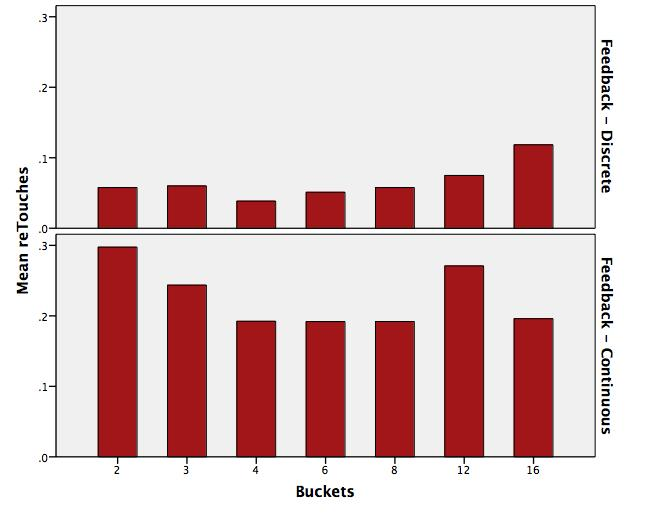
\includegraphics[scale=0.4]{figures/meanRetouches}
\caption{Target Re-Touches for Feedback Trials}
\label{fig:meanRetouches}
\end{figure}



%%%%%%%%%%%%%%%%%%%%%%%%%%%%%
%%%%%%%%%%%%%%%%%%%%%%%%%%%%%
%%%%%%%%%%%%%%%%%%%%%%%%%%%%%
%%%%%%%%%%%%%%%%%%%%%%%%%%%%%
%%%%%%%%%%%%%%%%%%%%%%%%%%%%%
%%%%%%%%%%%%%%%%%%%%%%%%%%%%%
\section{Subjective Preferences}
\label{resultsSubjectivePreferences}

In Figure \ref{fig:meanQuestGraphs}, the mean values for all the parts of the assessment presented in section \ref{assessment} are illustrated and presented. On each diagram the vertical axis represents the mean values of the corresponding category, which are ranged from 1 to 5 (5 point Likert scale). Generally, higher values mean that participants positively rated the specified category. The horizontal axis corresponds to the type of Trial. One (1) stands for Feedback \& Discrete Targeting, Two (2) for Feedback \& Continuous Targeting, Three (3) for No Feedback \& Discrete Targeting, and Four (4) for No Feedback \& Continuous Targeting. As a result each graph has 4 columns, identified with the numbers 1-4 ( from left to right).

\begin{figure}[H]
    \centering
    \begin{subfigure}[b]{0.4\textwidth}
        \centering
        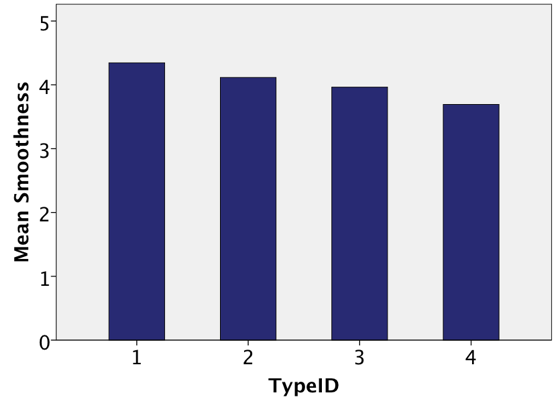
\includegraphics[width=\textwidth]{figures/meanSmoothness}
        \caption{Mean Smoothness}
        \label{fig:meanSmoothness}
    \end{subfigure}
    \hfill
    \begin{subfigure}[b]{0.4\textwidth}
        \centering
        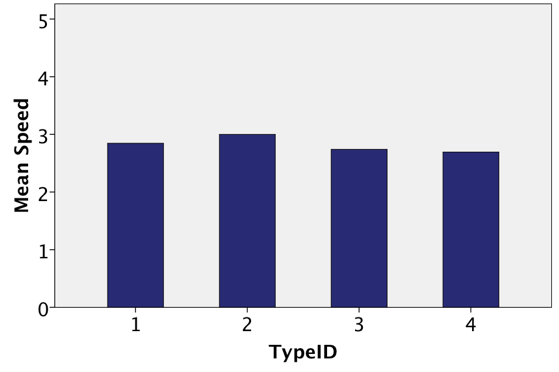
\includegraphics[width=\textwidth]{figures/meanSpeed}
        \caption{Mean Speed }
        \label{fig:meanSpeed}
    \end{subfigure}
    \hfill
    \begin{subfigure}[b]{0.4\textwidth}
        \centering
        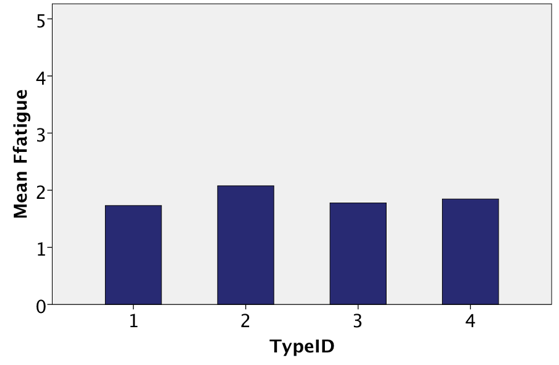
\includegraphics[width=\textwidth]{figures/meanFFatigue}
        \caption{Mean finger Fatigue}
        \label{fig:meanFFatigue}
    \end{subfigure}
    \hfill
    \begin{subfigure}[b]{0.4\textwidth}
        \centering
        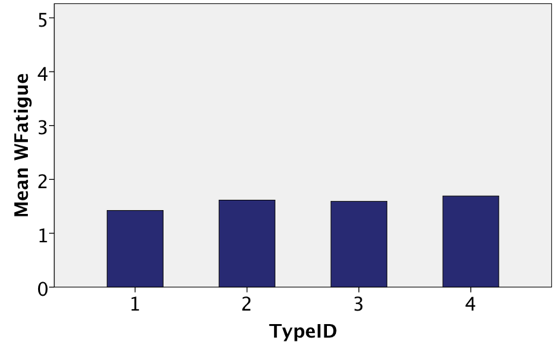
\includegraphics[width=\textwidth]{figures/meanWFatigue}
        \caption{Mean Wrist Fatigue}
        \label{fig:meanWFatigue}
    \end{subfigure}
    \hfill
    \begin{subfigure}[b]{0.4\textwidth}
        \centering
        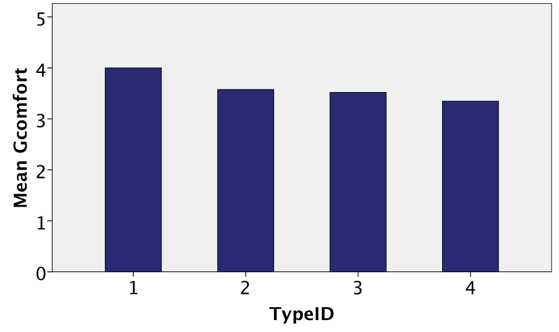
\includegraphics[width=\textwidth]{figures/meanGComfort}
        \caption{Mean Smoothness during operation}
        \label{fig:meanGComfort}
    \end{subfigure}
    \hfill
    \begin{subfigure}[b]{0.4\textwidth}
        \centering
        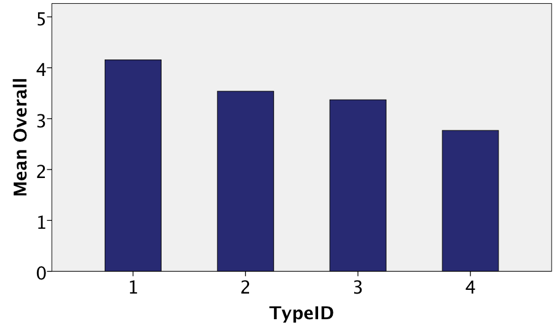
\includegraphics[width=\textwidth]{figures/meanOverall}
        \caption{Mean Overall Performance}
        \label{fig:meanOverall}
    \end{subfigure}
    \caption{Mean Values assessed by participants for each trial category}
    \label{fig:meanQuestGraphs}
\end{figure}

Feedback \& Discrete Targeting (1) scored consistently well across all the above categories. It scored mean values that were always improved than the ones of other trials. In most cases Feedback \& Discrete Targeting were following the queue, and the No Feedback ones were stacked behind.

Precisely, Feedback \& Discrete Targeting (1) was ranked higher concerning the Overall Performance (\emph{mean = 3.46 / 5}), Figure \ref{fig:meanOverall}. It can be observed that overall performance is decreased as the identification of the type of trial is increasing. The same behavior is also noticed for Mean Smoothness (\emph{mean = 4.03 / 5}), Figure \ref{fig:meanSmoothness}. However Most importantly, all four techniques ranked amazingly concerning the Fatigue of both the finger and the wrist. Even being an extensive and long experiment, which might not well correspond to everyday use scenario,  the fatigue  participants experienced was in extremely low levels. Finger fatigue had \emph{mean = 1.86}, as shown in Figure \ref{fig:meanFFatigue}, and Wrist fatigue also had \emph{mean = 1.58}, as shown in Figure \ref{fig:meanWFatigue}. Concerning Speed (\emph{mean = 2.82}), Figure \ref{fig:meanSpeed}, all techniques ranged quite uniformly, outlining that the operational speed of the experiment and of each technique in particular was mostly normal. Finally, Smoothness (\emph{mean = 4.03 / 5}), Figure \ref{fig:meanOverall}, ranged also very high for all techniques, which proves that our application is well structured and well corresponds to the movement of the finger.




% \begin{figure}[h]
% \centering
% 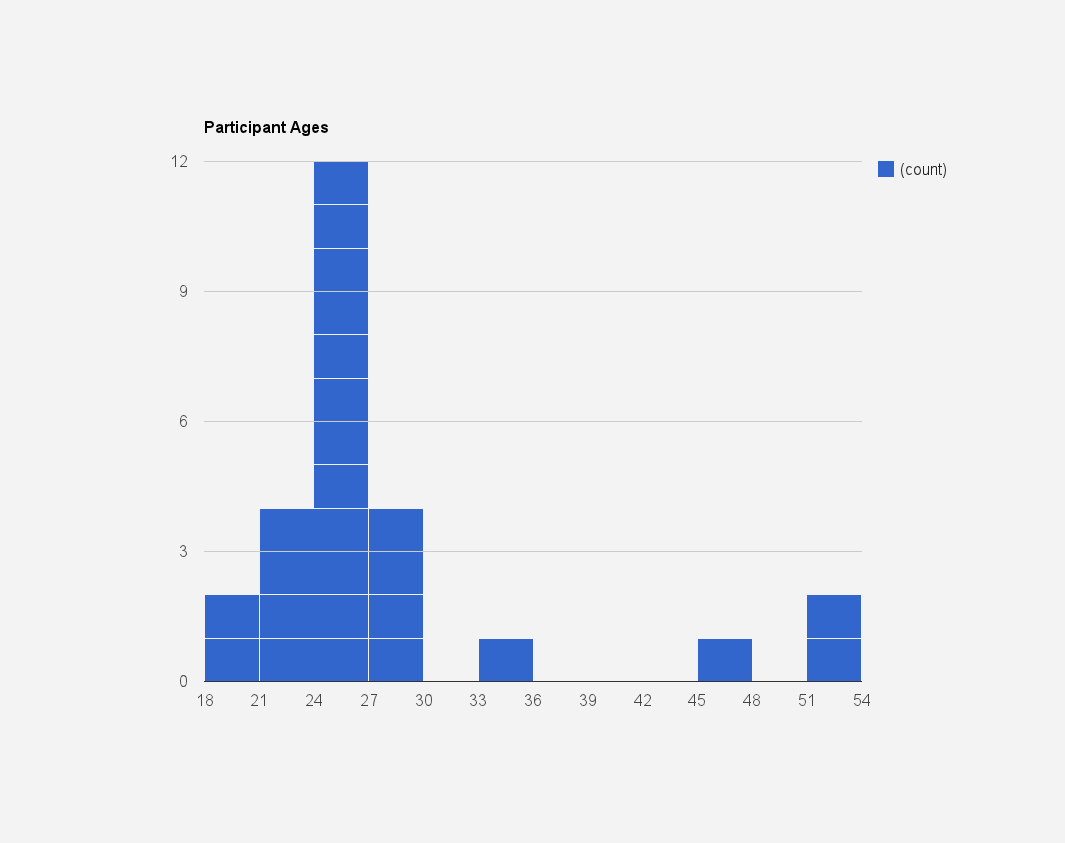
\includegraphics[scale=0.5]{figures/participantAge.png}
% \caption{Distribution of participant ages}
% \label{fig:participantAge}
% \end{figure}



% \begin{itemize}
% \item \textbf{}
% \item \textbf{}
% \item \textbf{}
% \item \textbf{}
% \end{itemize}
\cleardoublepage


\chapter{Discussion}
\label{sec:Discussion}
Conducting a study, without commenting and discussing on the results produced, does not make much os a sense. On Chapter \ref{sec:Experiment} (section \ref{sec:hypotheses}) we stated the hypotheses we made regarding this study. Then, on Chapter \ref{sec:Results} we presented, analysed and commented on all collected results, after separating them in six groups (Task Completion Time, Offsets, etc.). Now, we need to provide the necessary infrastructure to glue them together. That can be done by commenting and discussing if the hypotheses hold, taking into account the results we calculated. This is what this chapter is about; discuss, comment and reason whether the hypotheses stated, hold or not. Below, we are restating each of the hypotheses, along with discussing on their validity. 
 
\begin{itemize}

    %%%%%%%%
    %%%%%%%%
    %%%%%%%%
    \item \textbf{\textit{(H1). Feedback supplied trials (Discrete or Continuous) outperform No Feedback ones in terms of offset. }}

    In section \ref{sec:resultsOffset}, we mentioned that offset represents the error for each trial. The offset represents the distance (in percentage) between the point we selected and the center of the target. While No Feedback trials have no limitations on the value of the error, in Feedback \& Continuous trials the maximum allowed offset is \emph{+-2\%}.

    In chapter 6 we noted that, in No Feedback trials error rates were huge compared to the FeedBack Trials (only Feedback \& Continuous being considered). This was expected as in No Feedback trials, users have no indication on where is the feedback line; being also free, due to the QuickRelease technique, to lift their finger at whichever point (even if they are outside the target). Their ability to develop memory and predict correctly, was not enough to outperform Feedback trials. We can then conclude that, H1 holds.

    %%%%%%%%
    %%%%%%%%
    %%%%%%%%
    \item \textbf{\textit{(H2). No Feedback \& Discrete outperforms No Feedback \& Continuous in terms of offset.}}
    
    In section \ref{sec:resultsOffset} we mention that:
    \emph{Offset values for Discrete targeting are not always considered as errors, as we measure offset from the center of the targets range. The real error can be calculated by the type:}   $RealErrorDisrete = |OffsetValue| - (TargetRange*0.5)$

    On the results section, we noticed, much of our interest, that both NFD and NFC share the same error rates. Taking into account the aforementioned statement, that the Real Error in NFD trials is always smaller than offset we are provided with, we indeed realize that the real error in NFD trials is smaller than in NFC ones. As a result, H2 holds.

    %%%%%%%%
    %%%%%%%%
    %%%%%%%%
    \item \textbf{\textit{(H3). Task completion time will be gradually decreased over time.}}

    In other words, our hypothesis states that: 

    $AverageTimeRep1 > AverageTimeRep2 > AverageTimeRep3$ 

    In section \ref{sec:LCtotalTime} we presented and analysed the Task Completion Time Learning Curve. Learning curve is directly connected and related with the task completion time improvements over time. Taking into account the graphs presented in figure \ref{fig:learningCurveTotalTime}, we realize that there exist obvious learning improvements from repetition 1 to repetition 3, thus task completion time gradually decreases over time.  The only type of trials that we do not observe continuous improvement over time, is Feedback \& Continuous, for which in the 3rd repetition we have a slight increase of the average task completion time. As we also mentioned in section \ref{sec:LCtotalTime}, mental and physical fatigue might have a share in this behaviour, concluding that if it was not for fatigue (mental and physical), task completion time might have been further decreased on repetition 3. We can then conclude that hypothesis 3 for most type of trials.

    %%%%%%%%
    %%%%%%%%
    %%%%%%%%
    \item \textbf{\textit{(H4). Error rates will be gradually decreased over time.}}
    
    In section \ref{sec:LCOffset}, and more specific in Figure \ref{fig:learningCurveOffset} we observed that for all FC, NFD, NFC trials there exists a minor but almost unobservable error improvement over time, except probably for NFD. We observed that error rates slightly dropped on the second repetition, and remained stable or decreased in some cases on the third one. We can then conclude that, H4 is supported from the results, and thus it holds in general. 


    %%%%%%%%
    %%%%%%%%
    %%%%%%%%
    \item \textbf{\textit{(H5). Task competition time, when feedback is provided, is dependent on the number of elements.}}

    In section \ref{sec:resultsTaskCompletionTime} we made the following observations. When both Feedback and No Feedback trials are concerned, task completion time does not statistically differ for \emph{N = 2, 3, 4, 6, 8}. However we do observe a difference when $N=12$ or $N=16$. Thus H5 does not hold for all four different kinds of trials.
    However, addressing Feedback trials only, the scenery is alternated. For instance, for Feedback \& Discrete, completion time increases as the number of Elements increases. we observe $1.460 s$ for $N=2$, ending up with \emph{3.858 s} for $N=16$. As we have already mentioned, in Discrete trials, the number of elements (N) is highly related with the size of the target. However this does not hold for Continuous trials since there, N specifies the range of the position of the target. The size of a continuous target is fixed, and smaller than $N=16$ targets for Discrete trials. We indeed observed FC the completion time is stable and independent on the number of elements (\emph{N}), which makes sense exactly because in FC target size does not even change. Thus for FC trials, time is independent on the number of the elements, but is dependent of the size of the elements. Thus H5 holds only for FD trials, while if we modify it a bit it can also hold for FC trials. A modified version of H5 would be:

    \emph{Task competition time, when feedback is provided, is dependent on the \textbf{size of the target}.}




    %%%%%%%%
    %%%%%%%%
    %%%%%%%%
    \item \textbf{\textit{(H6). Average contact areas will be subconsciously preferred by users, as this is the natural position of the finger.}}
    
    If we observe Figure \ref{fig:meanOffset} in section \ref{sec:resultsOffset} we notice that in No Feedback trials, offset rates follow a common pattern. We experienced high positive offsets for targets located close to minimum contact area, almost zero offset when the target was located closed to the average contact area, and high negative offsets when target was located close to the maximum contact area. That, in other words means that, participants when not limited by the feedback line indicator, tent to subconsciously prefer and select contact areas that are closer to the average - median contact area. However when feedback is provided, they are forced by the application to precisely select the predefined target. That makes it impossible to study what H6 hypothesizes when we deal with Feedback trials. We then conclude, that when Feedback is not provided H6 holds.


    %%%%%%%%
    %%%%%%%%
    %%%%%%%%
    \item \textbf{\textit{(H7). Feedback \& Discrete is the most preferred type of trial, as it best combines speed and accuracy.}}

    In the additional assessment users provided us with (Appendix \ref{assessmentFatFinger}), we asked them to put the 4 different techniques in ascending order depending on which was the easiest to use. Users definitely preferred Feedback\&Discrete trials (as the easiest to use), with Feedback\&Continuous, No Feedback\&Discrete and Feedback\&Continuous following on the line. This definitely depicts user preferences, and if we also observe the results we got from the offset and completion time parameters, we realize that Feedback\&Discrete outperforms all other techniques regarding all measured parameters. Even for Task Completion time, in which due to the Dwell technique it requires an 1s delay to confirm target selection, the results are comparable to No Feedback trials, which in turn do not require any extra delays. As a result we can positively support that H7 holds.

\end{itemize}




Taking into consideration the above discussed hypotheses we perceive that all hypotheses hold, with minor modifications at certain cases. We note that \emph{Feedback \& Discrete} seems to be the most effective out of all types of trials, having comparable task completion time with No Feedback trials, almost overpassing the $1s$ obligatory delay obstacle. As discussed in section \ref{sec:resultsTaskCompletionTime}, task completion time does not statistically differ for N = 2, 3, 4, 6, 8. Thus we can conclude that users are able to distinguish up to 8 different discrete pressure levels when feedback is supplied, without any statistical significant difference on the task completion time. H7 further supports our claim, stating that FD is the most preferred selection technique, which also combines the best values for accuracy with a correspondent speed. 

We then observed that completion time for No Feedback trials is independent on the number of elements, $N$. Thus, performance can be mainly measured through the error rates. In section \ref{sec:LCOffset} we mentioned and commented on the error rates and the corresponding learning factor. 
We concluded that a level of 3, possibly 4, discrete levels is in turn identifiable and distinguishable by users, when feedback is not provided. 
H6 reveals that average contact areas are subconsciously preferred by users. This mainly happens because the natural position of the finger on the screen, requires an average contact size. This tendency is a significant parameter which contributes to the ability of No feedback trials to distinguish less discrete pressure levels; excluding the non-presence of the feedback region, which is the main and most important one.
We finally saw that the ability of a person to develop haptic memory to precisely select a target when N is very high, is limited. This further explains why the performance on No Feedback trials is decreased compared to the Feedback ones. 



\cleardoublepage

\chapter{Conclusion}

In this study we presented Fat Finger, an alternative interaction technique that uses the finger's contact size as the main source of input on a mobile or tablet device. The main objective of this study was to investigate how many distinguishable contact size levels can be actually achieved and perceived by users. 
In Chapter \ref{sec:Introduction} we introduced you to the current environment and developments on the market, explaining the limitations of the 2D interaction techniques, used to interact with the current smartphones and tablet devices. 
Then we broached you to the 3D interaction techniques, whose principle is to use the contact size of the finger touching the screen, in addition to it's position on the screen. In Chapter \ref{sec:RelatedWork} we presented all the relevant work and researches that have been already conducted on the same or highly related fields. We separated it in pressure-based and contact-shape-based approaches, thoroughly explaining similarities and differences with Fat Finger. 

In Chapter \ref{sec:FatFingerConcept} we presented the original idea behind Fat Finger interaction technique, along with the way we conceptualized its usage. Finally we raised the basic research question that this study will respond to, which is:
 \emph{"To which extend are we able to distinguish the different simulated pressure levels produced by our fingers using a tablet device?"}
The overall concept is that we want to investigate the capabilities and precision of using the contact area of the index finger  to interact with a tablet device. 

Chapter \ref{sec:Implementation} presents the interface the structure and the design of the application we developed to test and study Fat Finger interaction technique; it is in the form of discrete target selection trials, runs on and Apple iPad device, and consists of many consequent trials, each of them requiring the user to perform a target selection task.
First we explain the basic work-flow  we meet once we launch the application followed by the basic design and interface of a simple trial. Then we analyse the 4 categories of trials: Feedback \& Discrete, Feedback \& Continuous, No Feedback \& Discrete and  No Feedback \& Continuous. Finally, we explain the final sequence of the trials in the user study and the procedure and methods we used to monitor and measure user performance.
In Chapter \ref{sec:Experiment} we continue by analysing the procedure and the context of the user study. We had 26 participants taking part in this study.  Each user had to go through the verbal instructions, fill in the Demographic information form, calibrate his finger, accomplish the six hundred and twelve trials of the experiment, and finally fill in an assessment for each of the 4 different type of trials. We then gave statistical information regarding the demographic information of the participants that took place in our study. 

Finally, in Chapter \ref{sec:Results} we presented and discussed the computed results for all the basic parameters: Task completion time, Offset, Task Completion Time Learning Curve, Offset Learning Curve, Re-Entries and Re-Touches. Discussion on the results and arguing on the validity of the hypotheses stated in Chapter \ref{sec:Experiment}, are all performed in Chapter \ref{sec:Discussion}. We conclude that for Feedback supplied trials a level of 8 distinguishable contact size levels is easily perceived by users, while for No-Feedback ones we meet tolerated error rates only until 3 or 4 contact size levels. Also, we gave evidence and supported that all of the hypotheses we have set, hold.

While this study focuses on understanding touch and contact size on mobile devices, much work has to be done in order to produce real life products that will make use of this interaction technique. It will require the redesign of current interfaces, to make the cooperation with this technique feasible. But prior to redesigning the interface, we need to find the most appropriate way(s) to interact and exploit these multiple level contact size capabilities.

Thus next steps and future work will include the seek for a way to integrate this technique into on-market products. Fat Finger is capable to become both a sufficient alternative to the current gestured based approaches and also a much intuitive way to perform operations that are infeasible at the moment. 
One immediate way to integrate interaction through contact size with mobile interfaces is probably feasible by allowing the control of continuous variables through the variation of the contact size. For instance, volume, brightness, exposure etc. will now be controlled without the usage of a bar, which will not occupy any on-screen space. As a result, interfaces will be become simpler and more intuitive.
Another approach would be to use fingers to perform precise operation for which, currently, only pens are used. For the shake of illustration, S Pen is used by Samsung to perform operations that need augmented precision and detail. Is it possible, using Fat Finger, to achieve the same kind of detail through an interface which will provide us with the necessary infrastructure?
Finally, another suggestion is to study how FatFinger can be applied and integrated with multi-finger interaction. What is the impact on the ability to perceive the contact size levels, when multiple finger are used? What are the possible ways to combine current gestures with Fat Finger interaction technique? 
% Lets hope and that that in future, contact size based  input will become a standard on every day mobile interaction. 



\cleardoublepage

\bibliographystyle{plain}
\bibliography{bibliography/mendeley.bib,bibliography/external.bib}




\cleardoublepage

\appendix
\chapter{Verbal Istructions of Experiment}
\label{verbalFatFinger}
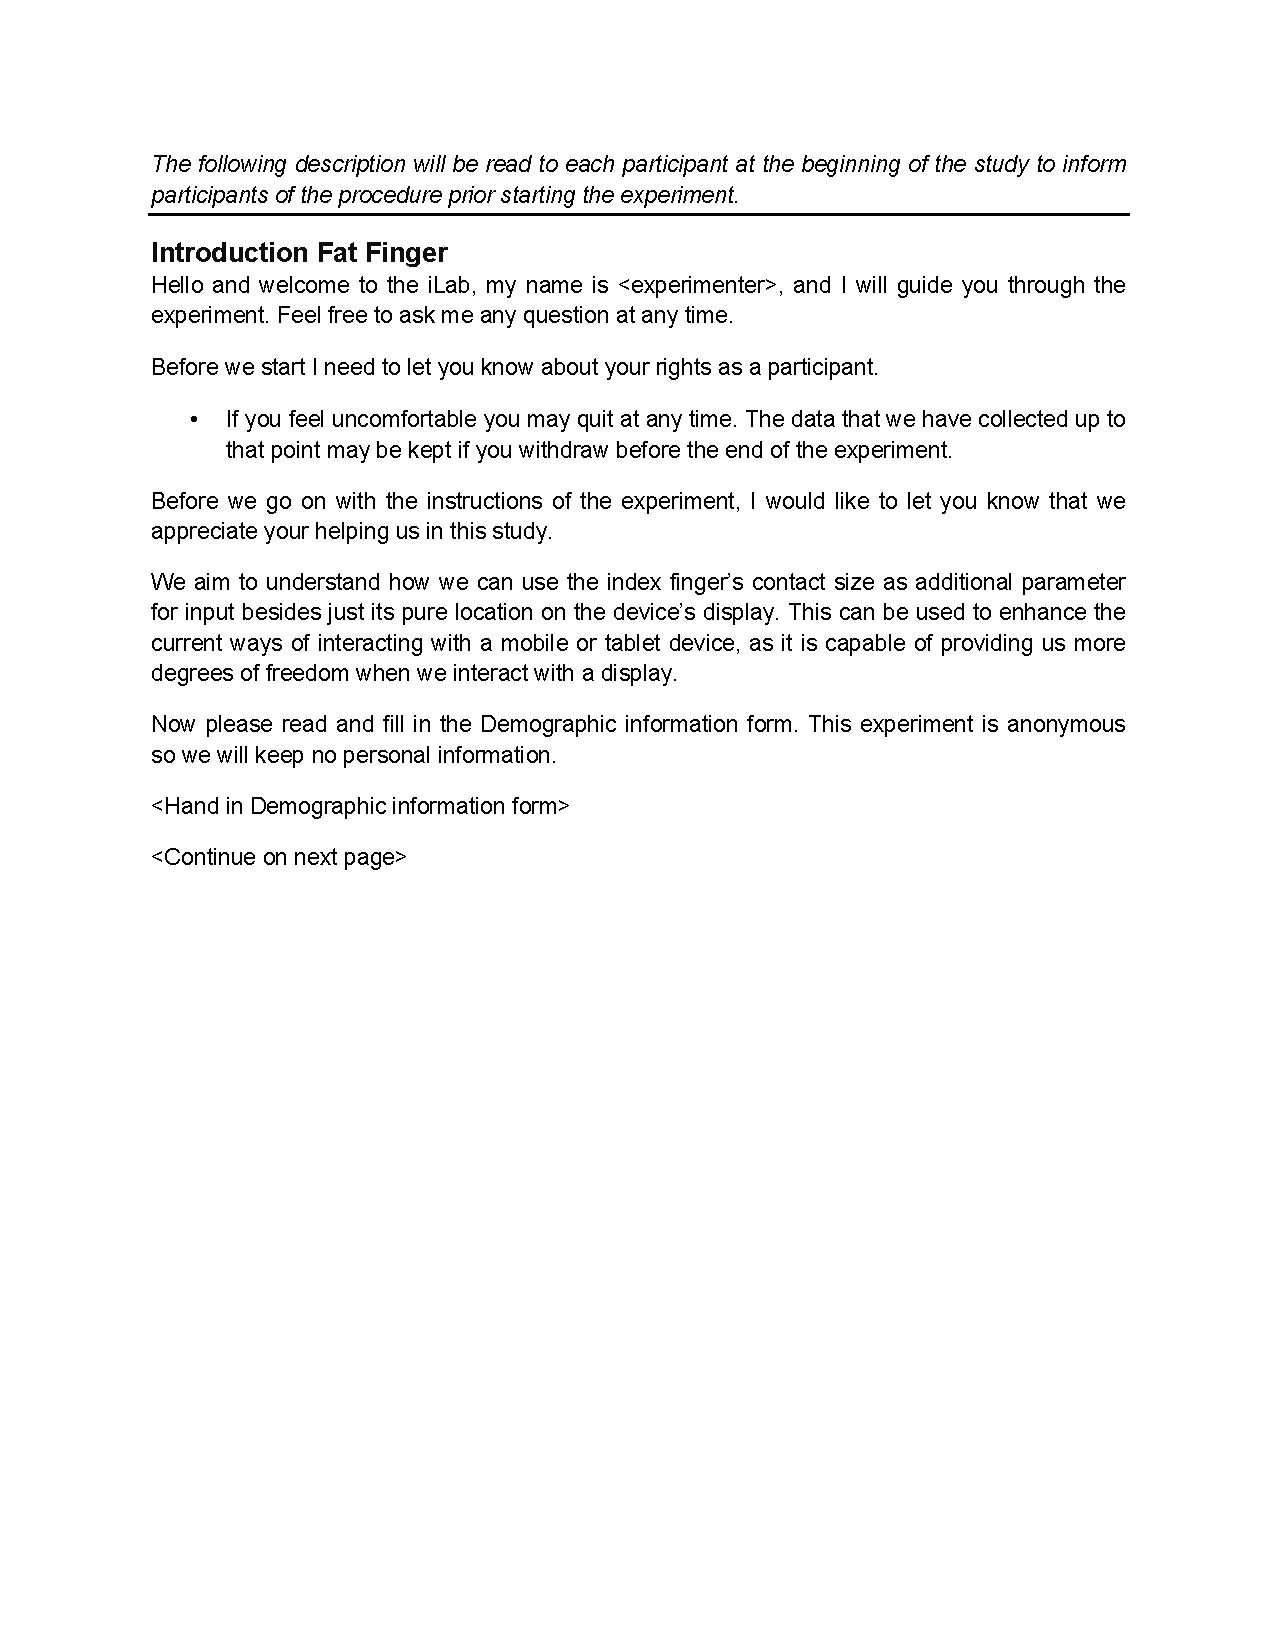
\includepdf[width=\textwidth,pages=-]{appendix/InstructionsFatFinger}

\chapter{Demographic Information Form}
\label{demographicFatFinger}
% 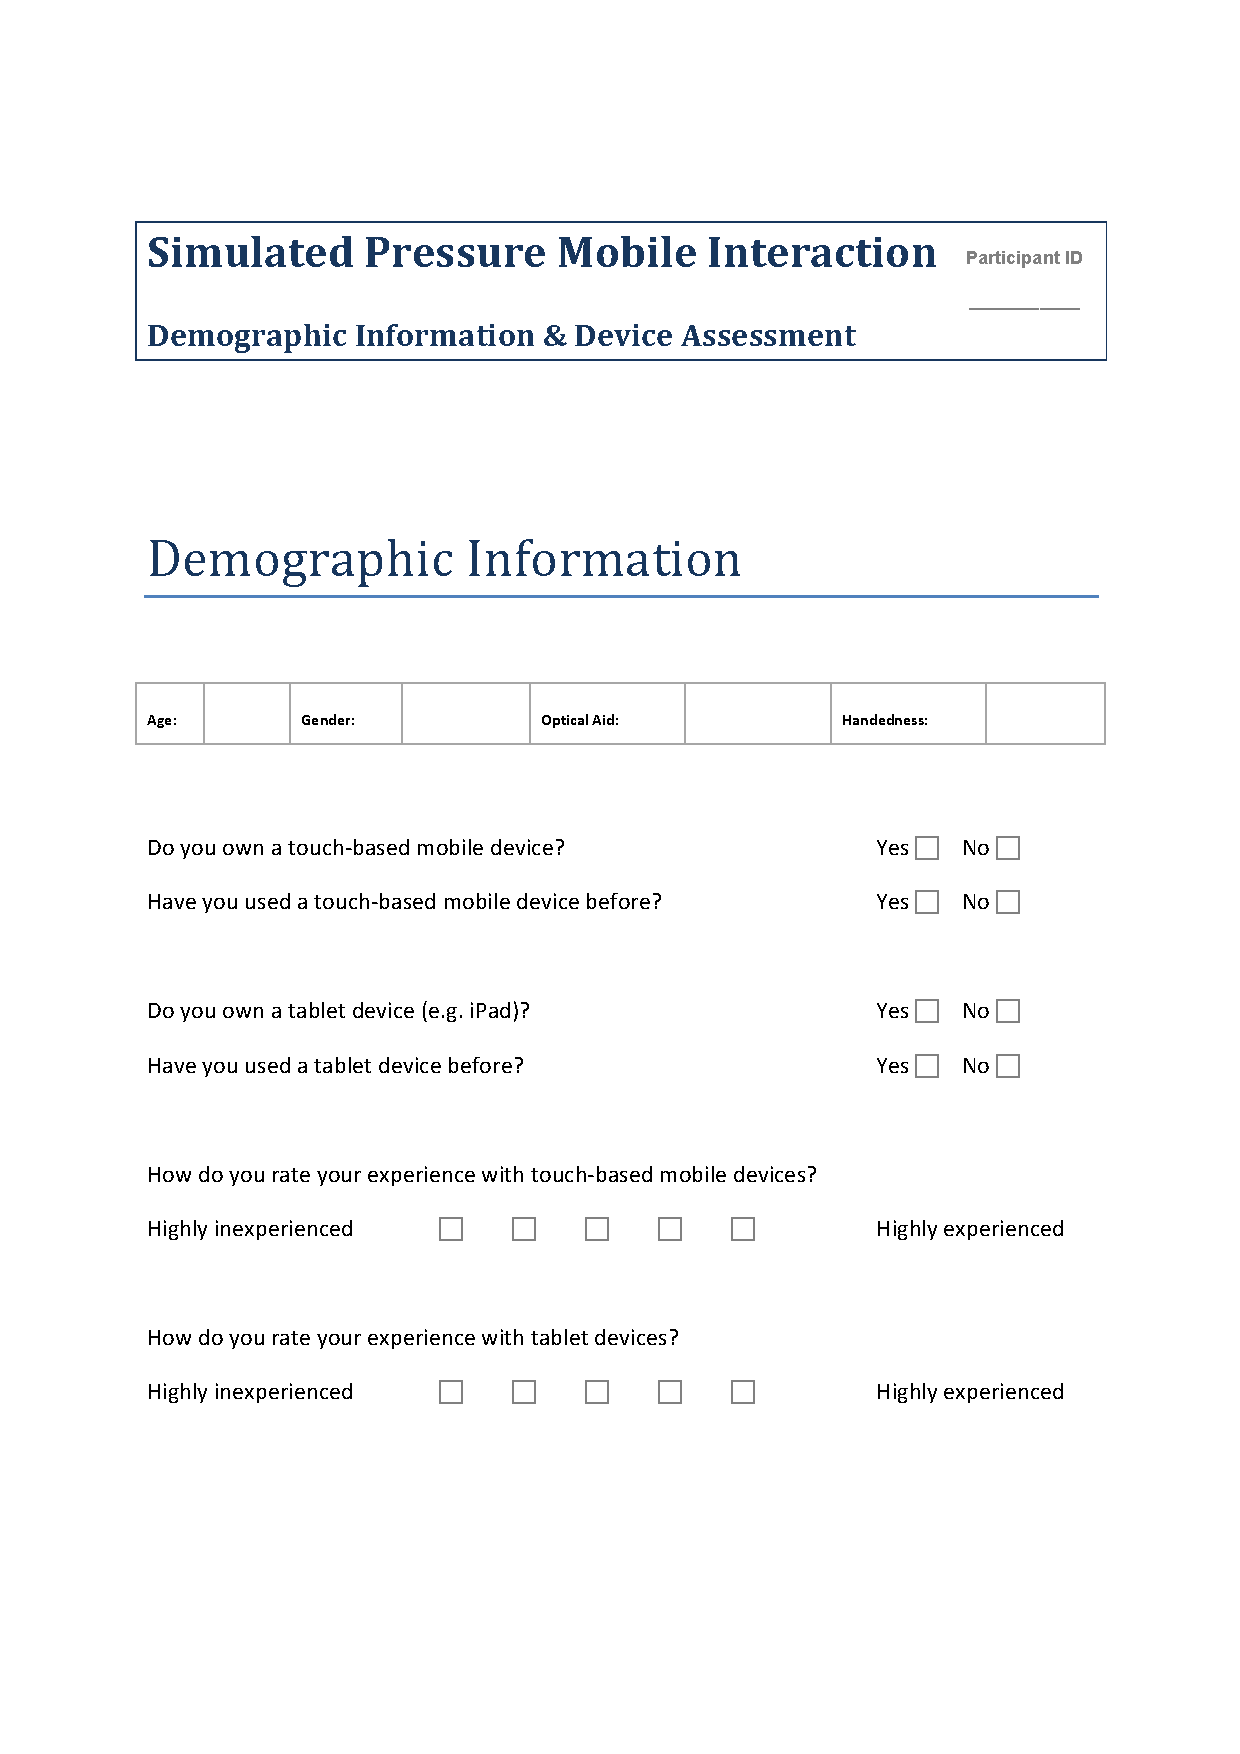
\includegraphics[width=\textwidth]{appendix/DemographicFatFinger}
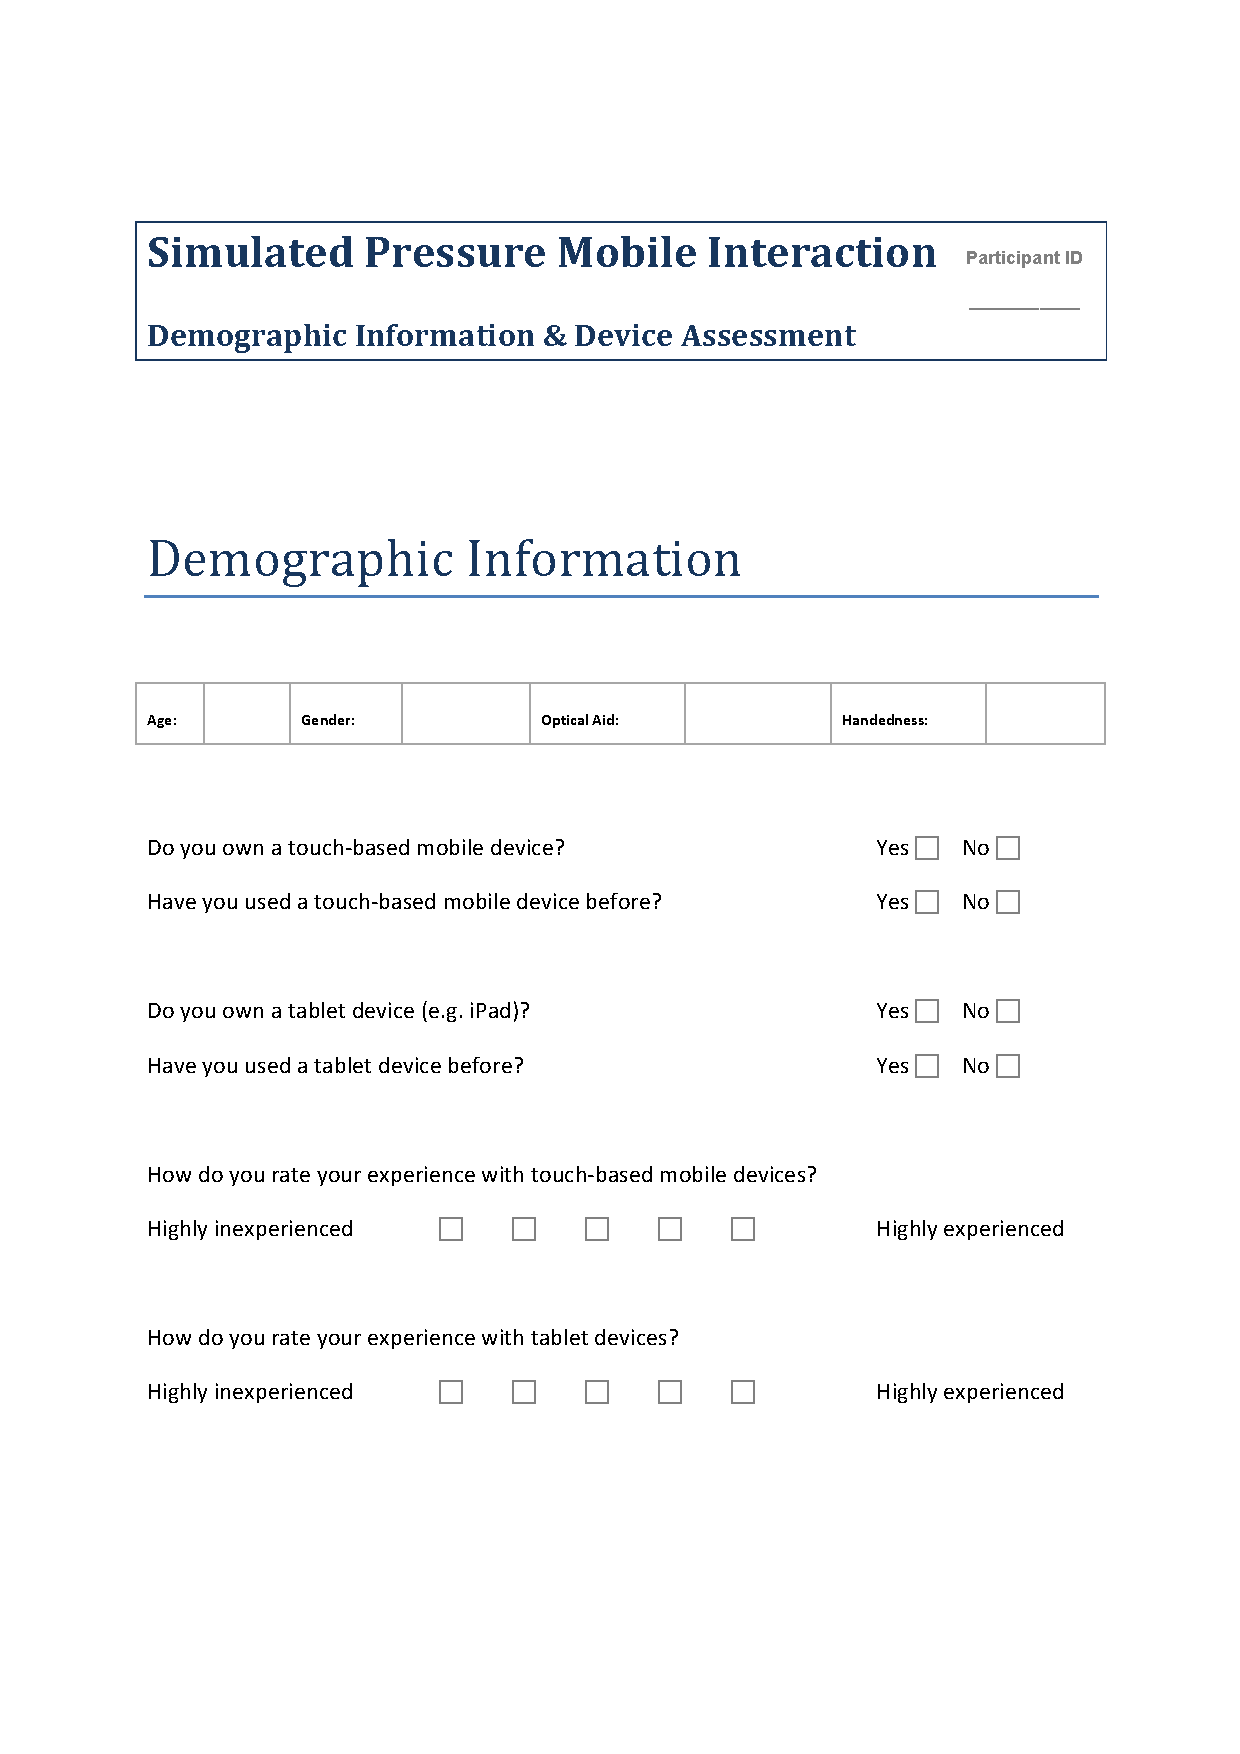
\includepdf[width=\textwidth,pages=-]{appendix/DemographicFatFinger}


\chapter{Technique Assessment Form}
\label{assessmentFatFinger}
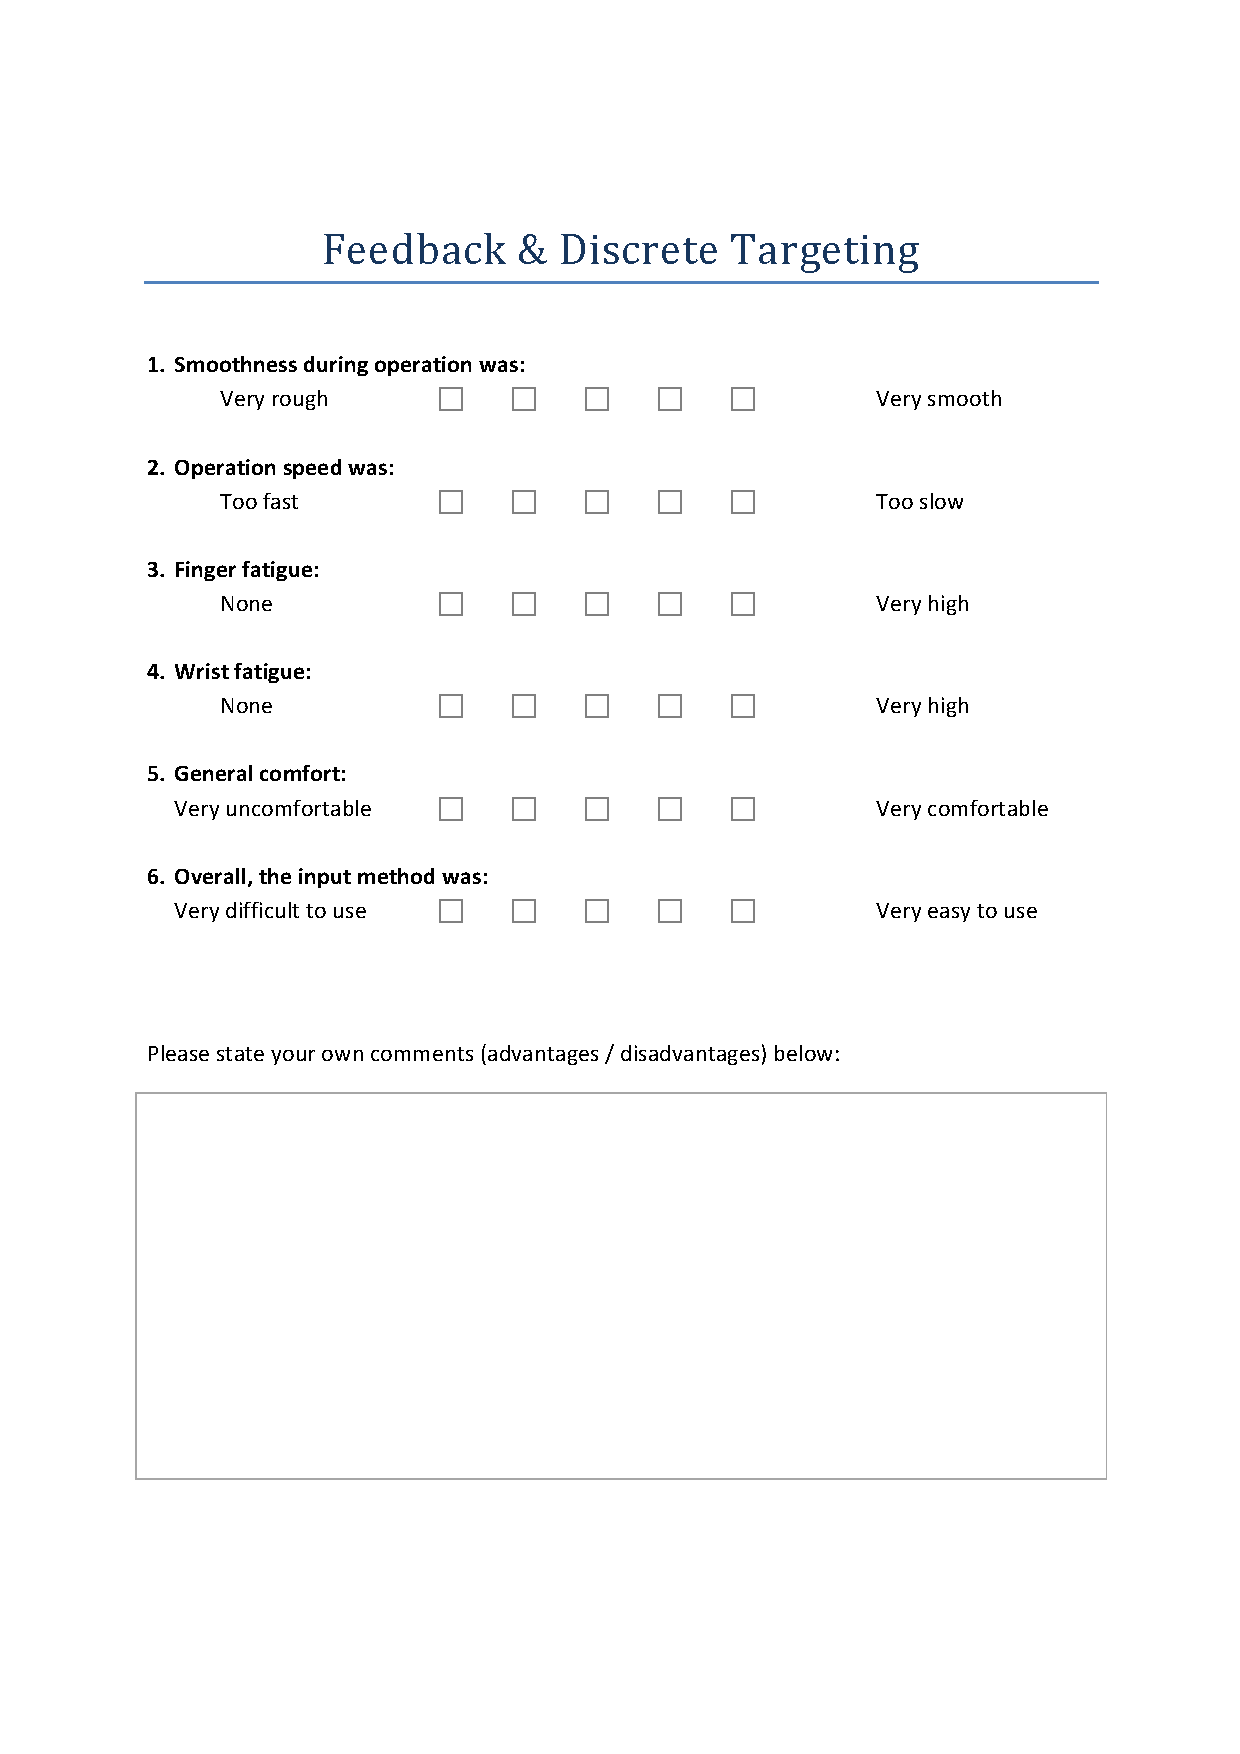
\includepdf[width=\textwidth,pages=-]{appendix/AssessmentFatFinger}
% 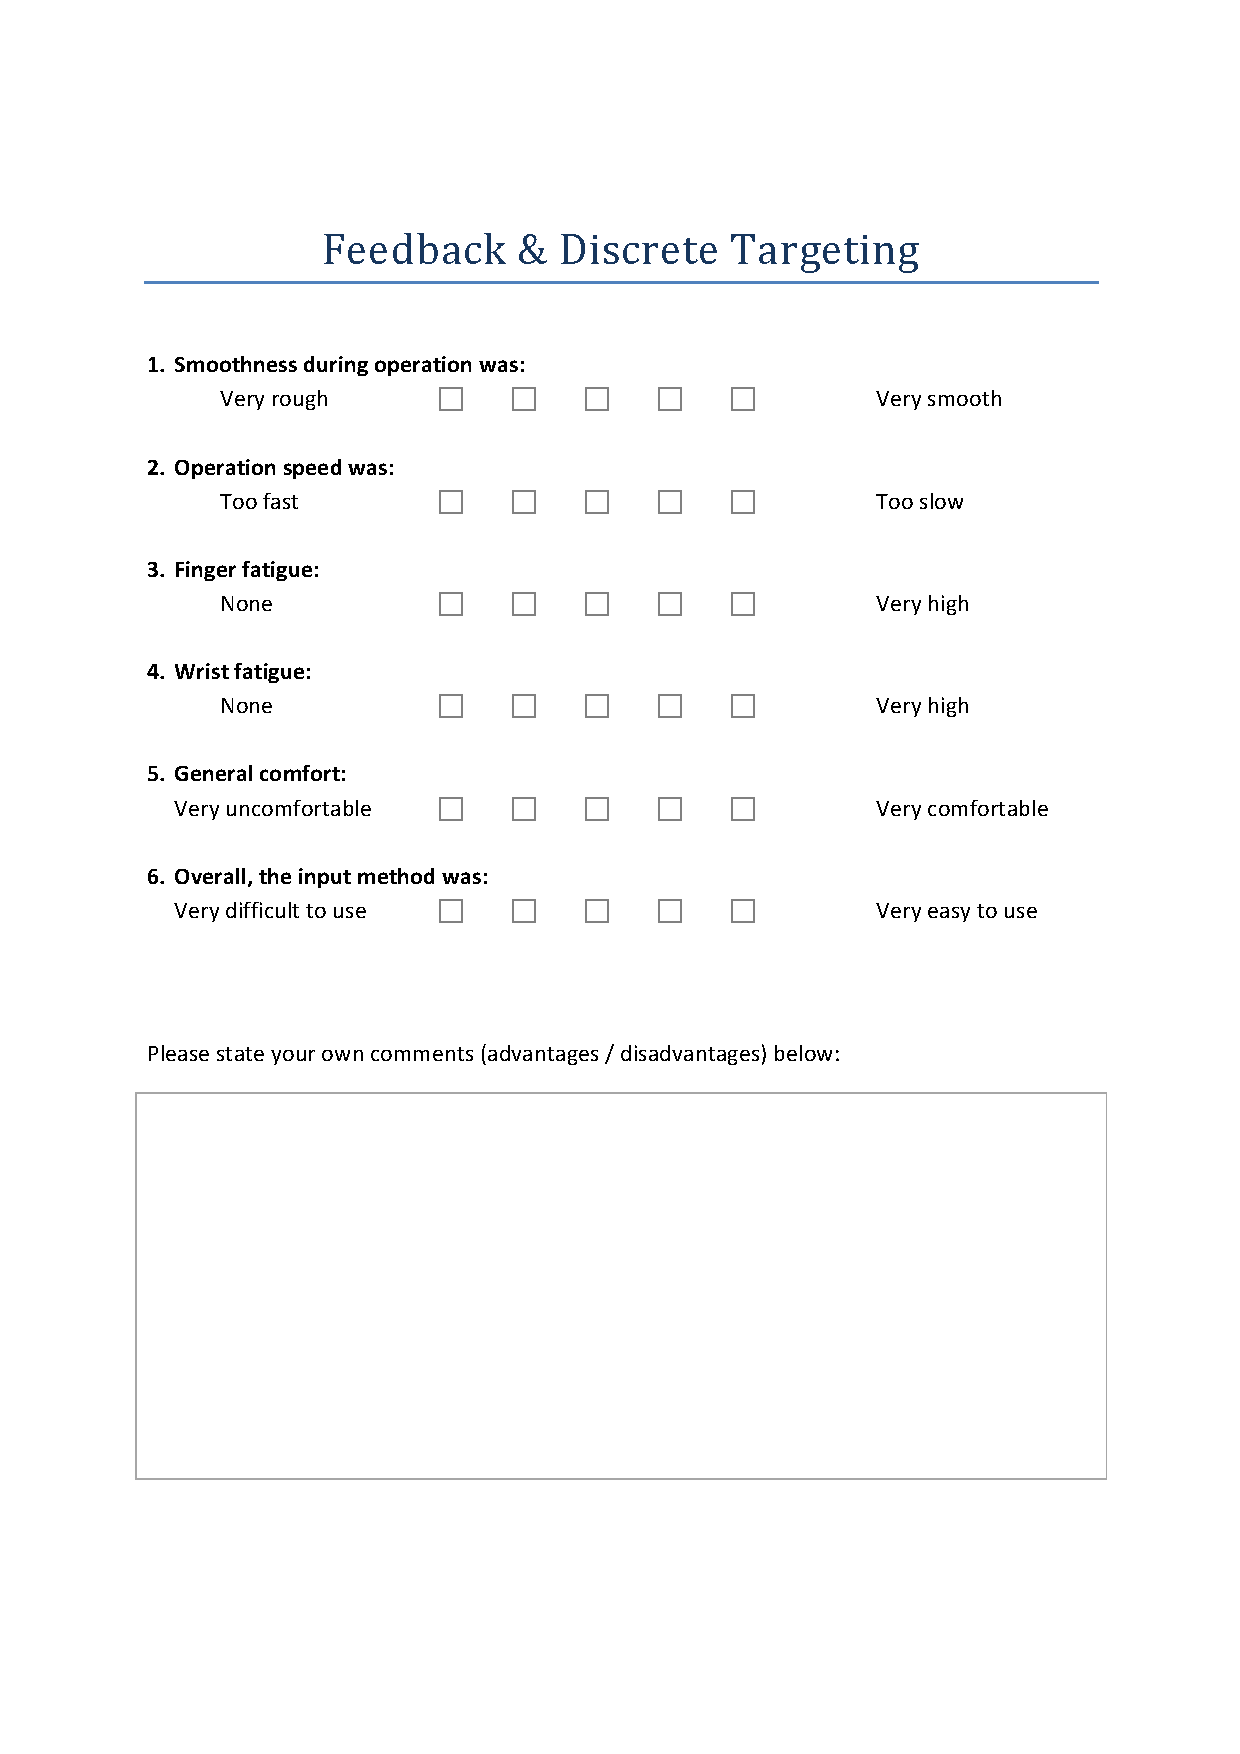
\includegraphics[width=\textwidth]{appendix/AssessmentFatFinger}



\end{document}

%%TODO: FIx [4] Reference
%% LATEX TUTORIAL
%https://www.sharelatex.com/blog/2013/08/09/thesis-series-pt5.html
